%%%%%%%%%%%%%%%%%%%%%%%%%%%%%%%%%%%%%%%%%%%%%%%%%%%%%%%%%%%%%%%%%%%%%%
%%  disstemplate.tex, to be compiled with latex.		     %
%%  08 April 2002	Version 4				     %
%%%%%%%%%%%%%%%%%%%%%%%%%%%%%%%%%%%%%%%%%%%%%%%%%%%%%%%%%%%%%%%%%%%%%%
%%								     %
%%  Writing a Doctoral Dissertation with LaTeX at		     %
%%	the University of Texas at Austin			     %
%%								     %
%%  (Modify this ``template'' for your own dissertation.)	     %
%%								     %
%%%%%%%%%%%%%%%%%%%%%%%%%%%%%%%%%%%%%%%%%%%%%%%%%%%%%%%%%%%%%%%%%%%%%%


\documentclass[12pt]{report}	% The documentclass must be ``report''.
  
\usepackage{utdiss2}  		% Dissertation package style file.

%%%%%%%%%%%%%%%%%%%%%%%%%%%%%%%%%%%%%%%%%%%%%%%%%%%%%%%%%%%%%%%%%%%%%%
% Optional packages used for this sample dissertation. If you don't  %
% need a capability in your dissertation, feel free to comment out   %
% the package usage command.					     %
%%%%%%%%%%%%%%%%%%%%%%%%%%%%%%%%%%%%%%%%%%%%%%%%%%%%%%%%%%%%%%%%%%%%%%

\usepackage{amsmath,amsthm,amsfonts,amscd} 
				% Some packages to write mathematics.
\usepackage{eucal} 	 	% Euler fonts
\usepackage{verbatim}      	% Allows quoting source with commands.
\usepackage{makeidx}       	% Package to make an index.
\usepackage{graphics}
\usepackage{psfig}         	% Allows inclusion of eps files.
\usepackage{epsfig}         	% Allows inclusion of eps files.
%\usepackage{citesort}         	% 
\usepackage{url}		% Allows good typesetting of web URLs.
%\usepackage{draftcopy}		% Uncomment this line to have the
				% word, "DRAFT," as a background
				% "watermark" on all of the pages of
				% of your draft versions. When ready
				% to generate your final copy, re-comment
				% it out with a percent sign to remove
				% the word draft before you re-run
				% Makediss for the last time.

\usepackage[T1]{fontenc}
\usepackage[scaled=0.95]{beramono}

\author{Analabha Roy}  	% Required

\address{4003 Red River St\\ Austin, Texas 78751}  % Required

\title{Dynamics of Quantum Control in Cold-Atom Systems}
                                                    % Required

%%%%%%%%%%%%%%%%%%%%%%%%%%%%%%%%%%%%%%%%%%%%%%%%%%%%%%%%%%%%%%%%%%%%%%
% NOTICE: The total number of supervisors and other members %%%%%%%%%%
%%%%%%%%%%%%%%% MUST be seven (7) or less! If you put in more, %%%%%%%
%%%%%%%%%%%%%%% they are put on the page after the Committee %%%%%%%%%
%%%%%%%%%%%%%%% Certification of Approved Version page. %%%%%%%%%%%%%%
%%%%%%%%%%%%%%%%%%%%%%%%%%%%%%%%%%%%%%%%%%%%%%%%%%%%%%%%%%%%%%%%%%%%%%

%%%%%%%%%%%%%%%%%%%%%%%%%%%%%%%%%%%%%%%%%%%%%%%%%%%%%%%%%%%%%%%%%%%%%%
%
% Enter names of the supervisor and co-supervisor(s), if any,
% of your dissertation committee. Put one name per line with
% the name in square brackets. The name on the last line, however,
% must be in curly braces.
%
% If you have only one supervisor, the entry below will read:
%
%	\supervisor
%		{Supervisor's Name}
%
% NOTE: Maximum three supervisors. Minimum one supervisor.
% NOTE: The Office of Graduate Studies will accept only two supervisors!
% 
%
\supervisor
	{Linda E. Reichl}

%%%%%%%%%%%%%%%%%%%%%%%%%%%%%%%%%%%%%%%%%%%%%%%%%%%%%%%%%%%%%%%%%%%%%%
%
% Enter names of the other (non-supervisor) members(s) of your
% dissertation committee. Put one name per line with the name
% in square brackets. The name on the last line, however, must
% be in curly braces.
%
% NOTE: Maximum six other members. Minimum zero other members.
% NOTE: The Office of Graduate Studies may restrict you to a total
%	of six committee members.
%
%
\committeemembers
        [C. Wendell Horton Jr.]
	[Qian Niu]
	[Mark G. Raizen]
	{Robert E. Wyatt}
%%%%%%%%%%%%%%%%%%%%%%%%%%%%%%%%%%%%%%%%%%%%%%%%%%%%%%%%%%%%%%%%%%%%%%

\previousdegrees{B.Sc.,M.Sc.}
     % The abbreviated form of your previous degree(s).
     % E.g., \previousdegrees{B.S., MBA}.
     %
     % The default value is `B.S., M.S.'

\graduationmonth{May}      
     % Graduation month, either May, August, or December, in the form
     % as `\graduationmonth{May}'. Do not abbreviate.
     %
     % The default value (either May, August, or December) is guessed
     % according to the time of running LaTeX.

\graduationyear{2009}   
     % Graduation year, in the form as `\graduationyear{2001}'.
     % Use a 4 digit (not a 2 digit) number.
     %
     % The default value is guessed according to the time of 
     % running LaTeX.

\typist{the author}       
     % The name(s) of typist(s), put `the author' if you do it yourself.
     % E.g., `\typist{Maryann Hersey and the author}'.
     %
     % The default value is `the author'.


%%%%%%%%%%%%%%%%%%%%%%%%%%%%%%%%%%%%%%%%%%%%%%%%%%%%%%%%%%%%%%%%%%%%%%
% Commands for master's theses and reports.			     %
%%%%%%%%%%%%%%%%%%%%%%%%%%%%%%%%%%%%%%%%%%%%%%%%%%%%%%%%%%%%%%%%%%%%%%
%
% If the degree you're seeking is NOT Doctor of Philosophy, uncomment
% (remove the % in front of) the following two command lines (the ones
% that have the \ as their second character).
%
%\degree{MASTER OF ARTS}
%\degreeabbr{M.A.}

% Uncomment the line below that corresponds to the type of master's
% document you are writing.
%
%\masterreport
%\masterthesis


%%%%%%%%%%%%%%%%%%%%%%%%%%%%%%%%%%%%%%%%%%%%%%%%%%%%%%%%%%%%%%%%%%%%%%
% Some optional commands to change the document's defaults.	     %
%%%%%%%%%%%%%%%%%%%%%%%%%%%%%%%%%%%%%%%%%%%%%%%%%%%%%%%%%%%%%%%%%%%%%%
%
%\singlespacing
%\oneandonehalfspacing

%\singlespacequote
\oneandonehalfspacequote

\topmargin 0.125in	% Adjust this value if the PostScript file output
			% of your dissertation has incorrect top and 
			% bottom margins. Print a copy of at least one
			% full page of your dissertation (not the first
			% page of a chapter) and measure the top and
			% bottom margins with a ruler. You must have
			% a top margin of 1.5" and a bottom margin of
			% at least 1.25". The page numbers must be at
			% least 1.00" from the bottom of the page.
			% If the margins are not correct, adjust this
			% value accordingly and re-compile and print again.
			%
			% The default value is 0.125"

		% If you want to adjust other margins, they are in the
		% utdiss2-nn.sty file near the top. If you are using
		% the shell script Makediss on a Unix/Linux system, make
		% your changes in the utdiss2-nn.sty file instead of
		% utdiss2.sty because Makediss will overwrite any changes
		% made to utdiss2.sty.

%%%%%%%%%%%%%%%%%%%%%%%%%%%%%%%%%%%%%%%%%%%%%%%%%%%%%%%%%%%%%%%%%%%%%%
% Some optional commands to be tested.				     %
%%%%%%%%%%%%%%%%%%%%%%%%%%%%%%%%%%%%%%%%%%%%%%%%%%%%%%%%%%%%%%%%%%%%%%

% If there are 10 or more sections, 10 or more subsections for a section,
% etc., you need to make an adjustment to the Table of Contents with the
% command \longtocentry.
%
%\longtocentry 



%%%%%%%%%%%%%%%%%%%%%%%%%%%%%%%%%%%%%%%%%%%%%%%%%%%%%%%%%%%%%%%%%%%%%%
%	Some math support.					     %
%%%%%%%%%%%%%%%%%%%%%%%%%%%%%%%%%%%%%%%%%%%%%%%%%%%%%%%%%%%%%%%%%%%%%%
%
%	Theorem environments (these need the amsthm package)
%
%% \theoremstyle{plain} %% This is the default

\newtheorem{thm}{Theorem}[section]
\newtheorem{cor}[thm]{Corollary}
\newtheorem{lem}[thm]{Lemma}
\newtheorem{prop}[thm]{Proposition}
\newtheorem{ax}{Axiom}

\theoremstyle{definition}
\newtheorem{defn}{Definition}[section]

\theoremstyle{remark}
\newtheorem{rem}{Remark}[section]
\newtheorem*{notation}{Notation}

%\numberwithin{equation}{section}


%%%%%%%%%%%%%%%%%%%%%%%%%%%%%%%%%%%%%%%%%%%%%%%%%%%%%%%%%%%%%%%%%%%%%%
%	Macros.							     %
%%%%%%%%%%%%%%%%%%%%%%%%%%%%%%%%%%%%%%%%%%%%%%%%%%%%%%%%%%%%%%%%%%%%%%
%
%	Here some macros that are needed in this document:


\newcommand{\latexe}{{\LaTeX\kern.125em2%
                      \lower.5ex\hbox{$\varepsilon$}}}

\newcommand{\amslatex}{\AmS-\LaTeX{}}

\chardef\bslash=`\\	% \bslash makes a backslash (in tt fonts)
			%	p. 424, TeXbook

\newcommand{\cn}[1]{\texttt{\bslash #1}}

\makeatletter		% Starts section where @ is considered a letter
			% and thus may be used in commands.
\def\square{\RIfM@\bgroup\else$\bgroup\aftergroup$\fi
  \vcenter{\hrule\hbox{\vrule\@height.6em\kern.6em\vrule}%
                                              \hrule}\egroup}
\makeatother		% Ends sections where @ is considered a letter.
			% Now @ cannot be used in commands.

\makeindex    % Make the index

%%%%%%%%%%%%%%%%%%%%%%%%%%%%%%%%%%%%%%%%%%%%%%%%%%%%%%%%%%%%%%%%%%%%%%
%		The document starts here.			     %
%%%%%%%%%%%%%%%%%%%%%%%%%%%%%%%%%%%%%%%%%%%%%%%%%%%%%%%%%%%%%%%%%%%%%%

\begin{document}

\copyrightpage          % Produces the copyright page.


%
% NOTE: In a doctoral dissertation, the Committee Certification page
%		(with signatures) is BEFORE the Title page.
%	In a masters thesis or report, the Signature page
%		(with signatures) is AFTER the Title page.
%
%	If you are writing a masters thesis or report, you MUST REVERSE
%	the order of the \commcertpage and \titlepage commands below.
%
\commcertpage           % Produces the Committee Certification
			%   of Approved Version page (doctoral)
			%   or Signature page (masters).
			%		20 Mar 2002	cwm

\titlepage              % Produces the title page.



%%%%%%%%%%%%%%%%%%%%%%%%%%%%%%%%%%%%%%%%%%%%%%%%%%%%%%%%%%%%%%%%%%%%%%
% Dedication and/or epigraph are optional, but must occur here.      %
%%%%%%%%%%%%%%%%%%%%%%%%%%%%%%%%%%%%%%%%%%%%%%%%%%%%%%%%%%%%%%%%%%%%%%
%
\begin{dedication}
\index{Dedication@\emph{Dedication}}%
Dedicated to my father, Professor. Probir Roy.
\end{dedication}


\begin{acknowledgments}		% Optional
\index{Acknowledgments@\emph{Acknowledgments}}%
I am indebted to my advisor, Linda Reichl, for her guidance, support and patience. When I approached her expressing interest in the dynamics of cold atom systems, her previous research in this area provided invaluable insights and resulted in quickly specifying the problems tackled in this dissertation. She has given me considerable latitude and freedom in my research, and supported it intellectually and financially. Errors and misconceptions were efficiently identified and corrected, thanks in no small part to her penetrating critiques and extensive expertise in these areas. Her guidance led this research to be deemed valuable to the scientific community, and resulted in considerable satisfaction on our part at the completion of this work.

I am also grateful to the assistance of Dr. Kyungsun Na at the Center for Complex Quantum systems. Her research work in the dynamics of quantum control in molecular systems was the stepping stone that set us on the journey into the problems tackled here in this dissertation. The numerical tools and techniques that she developed were of great help with these problems. I would also like to take this opportunity to extend my gratitude to Dr. Benjamin P Holder. His works regarding the dynamics of noninteracting cold atom systems were the shoulders of the giant from which this bird flew to the skies. My thanks also extend to Professors Dicus, MacDonald, and Niu here at UT for their courses, and to Professor Mark Raizen for his critical eye and knowledge that was of considerable help. Annie Harding at the Center for Complex Quantum Systems has always provided me with reliable assistance in going through the red tape.

In order to reach this point in my academic life, I have gone through many stepping stones. At each stage, obstacles were encountered and surmounted as part of a rich tapestry of science and intellect that has been a vital part of my life. This treatise would be woefully incomplete without acknowledging those teachers that have informed and inspired my interest in physics, and provided me with the experience and background needed to get this far. My thanks go out to Professor Soumitra 'Akuda' Sengupta (formerly) of Jadavpur University, Calcutta, whose superlative introductory and intermediate courses in statistical mechanics were where I was taught almost everything that I needed to know in order to get started, not just basic principles but the right frame of mind and attitude needed to solve problems. I cannot over-stress his influence as a great teacher, and his enormous passion for physics that excited and inspired so many of his students, including myself. 

In addition, I happily acknowledge the influence of Professor Jayanta Bhattacharjee of the Indian Association for the Cultivation of Science, Calcutta, for introducing me to the world of the dynamics of complex systems and chaos, as well as the world of cutting-edge research in these areas. I would also like to thank Professor Sreerup Raychaudhuri of the Indian Institute of Technology, Kanpur, whose courses in quantum mechanics and field theory were to me what Akuda's courses were in statistical mechanics. His instruction, as well as moral support, got me through some difficult times. Also, my thanks to Professor Debashish Chowdhuri of I.I.T. Kanpur for his difficult but informative course on advanced statistical mechanics.

Lastly, I would like to thank my parents, my father, Professor Probir Roy and  mother, Professor Manashi Roy (retd). My father, a particle physicist, was my primary influence in all things. He taught me all the fundamental physics that I know. My mother has supported me at every turn and her love kept me going.

\end{acknowledgments}


% The abstract is required. Note the use of ``utabstract'' instead of
% ``abstract''! This was necessary to fix a page numbering problem.
% The abstract heading is generated automatically.
% Do NOT use \begin{abstract} ... \end{abstract}.
%
\utabstract
\index{Abstract}%
\indent
The dynamics of mesoscopic two-boson systems that model an interacting pair of ultracold alkali atoms in the presence of electromagnetic potentials are considered. The translational degrees of freedom of such a system can be described by a simple reduced atom Hamiltonian. Introducing time modulations in the laser fields causes parametric variations of the Hamiltonian's Floquet eigenvalue spectrum. Broken symmetries cause level repulsion and avoided crossings in this spectrum that are quantum manifestations of the chaos in the underlying classical dynamics of the systems. We investigate the effects of this phenomenon in the coherent control of excitations in these systems. These systems can be coherently excited from their ground states to higher energy states via a Stimulated Raman Adiabatic Passage (STIRAP). The presence of avoided crossings alter the outcome of STIRAP. First, the classical dynamics of such two-boson systems in double wells is described and manifestations of the same to the quantum mechanical system are discussed. Second, the quantum dynamics of coherent control in the manner discussed above is detailed for a select choice(s) of system parameters. Finally, the same chaos-assisted adiabatic passage is demonstrated for optical lattice systems based on experiments on the same done with noninteracting atoms.

\tableofcontents   % Table of Contents will be automatically
                   % generated and placed here.

\listoftables      % List of Tables and List of Figures will be placed
\listoffigures     % here, if applicable.



%%%%%%%%%%%%%%%%%%%%%%%%%%%%%%%%%%%%%%%%%%%%%%%%%%%%%%%%%%%%%%%%%%%%%%
% Actual text starts here.					     %
%%%%%%%%%%%%%%%%%%%%%%%%%%%%%%%%%%%%%%%%%%%%%%%%%%%%%%%%%%%%%%%%%%%%%%
%
% Including external files for each chapter makes this document simpler,
% makes each chapter simpler, and allows for generating test documents
% with as few as zero chapters (by commenting out the include statements).
% This allows quicker processing by the Makediss command file in case you
% are not working on a specific, long and slow to compile chapter. You
% can even change the chapter order by merely interchanging the order
% of the include statements (something I found helpful in my own
% dissertation).
%
\chapter{Introduction}
\index{Introduction@\emph{Introduction}}%
\label{chapter-intro}
There have been significant advancements in  techniques for cooling and trapping ultracold atom gases in recent years. Modern techniques allow for the removal of thermal effects on the atoms by cooling them to near absolute zero temperatures. This facilitated the experimental realization of Bose-Einstein condensation in  dilute alkali gases (specifically $^{85}Rb$ and $^{23}Na$) in 1995~\cite{weiman}~\cite{weiman:cornell}~\cite{ketterle}~\cite{ketterle2}. Since then, numerous studies of these condensates have been accomplished. In addition, experiments have been conducted that have obtained boson systems in number squeezed states from ultracold gases of alkali atoms in optical traps~\cite{raizen}. Thus, it is now possible to create a mesoscopic two-boson system of Sodium or Rubidium. Individual alkali atoms from a BEC reservoir can be subjected to quantum tweezers (Gaussian lasers exploiting the Landau-Zener tunneling between the reservoir levels and the levels in the laser beam)~\cite{diener}. Other recent methods include number-squeezing the BEC itself by "culling" atoms from a trapped condensate down to a sub-poissonian regime, making the number uncertainty small enough to be ignored~\cite{raizen}~\cite{Dudarev:Raizen:Niu}. In addition, cooled and trapped atoms can be subjected to electromagnetic fields, such as counter-propagating beams of lasers producing a one dimensional 'optical lattice'. In such systems, only the translational degrees of freedom of the center of mass of the atoms contribute to the dynamics via an effective Hamiltonian~\cite{graham}. Arrays of number squeezed atoms can be subjected to optical lattices where  the potential at each site can be tuned to the desired profile, including the double well systems which will be the main focus of this dissertation~\cite{Deutsch:Jessen}. Double-well systems can also be designed for cold atoms using atom chips that generate magnetic fields, trapping the system using the Zeeman effect~\cite{doublewell:chip}~\cite{doublewell:chip:nature}.

The Hamiltonians that we will be studying here are one-dimensional and time periodic, with kinetic energy and potential energy that follows the intensity profile of the confining field(s). The time-periodicity gives us the ability to use Floquet theory to find solutions to the Schr\"odinger equation that are of the same time period and modulated by Floquet quasienergies. The same problem can also be solved by transforming to a time-folded \textit{composite Hilbert space} built from the space of all functions that are square-integrable in space as well as the time period. The transformed 'Floquet Hamiltonian' has the Floquet quasienergies and periodic Floquet solutions described above as its actual eigensystem, and that eigensystem describes the complete dynamics of the system.

The effective interaction between the atoms comes from the s-wave scattering amplitude, and is a point contact pseudopotential~\cite{metcalf:vanderstraten}~\cite{pethick:bec}. The nonlinear resonances from this pseudopotential create large chaotic regions in the classical phase space~\cite{reichl}. Nonlinear resonances that create chaos also comes from time-dependent drives, much like it does with the duffing oscillator. 

The  goal of this research has been to determine how the quantum dynamics is affected by the underlying classical chaos in these interacting mesoscopic systems once they have been reduced to zero-dimensional problems. The main influence of classical chaos in the quantum dynamics comes from the loss in symmetry from the non-integrability, which breaks degeneracies in the Floquet quasienergies, leading to avoided crossings in the parameter space in non-integrable regions. We investigate the influence of these avoided crossings when performing resonant excitations of the system from the ground state to excited states. Avoided crossings can be created by harmonically coupling the energy levels of the time-independent Hamiltonian and performing coherent excitations via Stimulated Raman Adiabatic Passage (STIRAP). The underlying chaos will produce avoided crossings in the Floquet eigenspace that affect the outcome of the STIRAP depending on whether the time scale of the dynamics is slow enough for a chaos assisted adiabatic passage to occur.

The dissertation is organized as follows. Chapter~\ref{chapter-dblwell} covers the dynamics of coherent quantum control of the type described above for two alkali metal bosons confined in a double well. The classical dynamics of the undriven system is described in detail. The wavefunctions of the stationary states for the system are obtained and their representations in the quantum phase space compared with the classical dynamics. The system is then subjected to time-modulated radiation pulses so as to induce Raman excitations of the type described above. The Floquet theory required for the analysis of the quantum dynamics of such excitations is also detailed. Computational calculations of the Floquet eigenspace is shown for suitable parameters, and the results compared with numerical simulations of the actual quantum time evolution. Chapter~\ref{chapter-optical_lattice} covers the dynamics of 2 alkali metal bosons confined to a simple pendulum-like optical lattice where the atoms have been loaded to allow for periodic boundary conditions over small periods of the lattice. The lattice is subjected to a 3-resonance type time dependence where two identical copies of the lattice are set to counter-propagate at the same speed, producing a stationary periodic time dependence that can be modulated such that STIRAP can be achieved. The dynamics of the coherent quantum control of excitations are analyzed in the same manner as that of the double well system in chapter~\ref{chapter-dblwell}. Concluding remarks are made in the final chapter. The appendices contain detailed information that is required for the numerical computations, as well as some material concerning the time-of-flight signatures of the double well states.

The rest of this chapter provides the background necessary for subsequent chapters. The next section will give a brief introduction to the theory of atomic interactions with classical electromagnetic fields. The following section will provide some background material concerning the dynamics of two-level systems at symmetry-breaking avoided crossings. The final section will describe a theoretical treatment of the three level STIRAP problem which will be the form of quantum control that we have employed for cold atom systems.

\section{Semiclassical Interactions between Atoms and Electromagnetic Fields}
\label{chapter-intro:section:lightatom}
A short introduction to the theory of the semi classical interaction between matter and electromagnetic interactions is provided here. Neutral atoms do not couple directly to electromagnetic fields on account of having no total charge. However, they do have multipole moments, and they cause the atom dynamics to be affected by electromagnetic fields. The multipole moments are quantum mechanical in origin, and are obtained from the internal atomic states. The historic Stern-Gerlach experiment used this property to separate the spins of a stream of atoms~\cite{sakurai}. Our primary interests in this dissertation are the optical dipole force, which is used in optical dipole traps (O.D.T.) to confine the translational degrees of freedom of ultracold alkali metal atoms, and the magnetic Zeeman force, which are used in magnetic atom chip systems to do the same. 

The far-off-resonance optical traps or FORTS employ the use of conservative forces whereby light detuned away from the internal atomic resonances with spatially varying intensities create an effective Hamiltonian for the confining atom whose potential curve adiabatically traces the intensity profile of the beam.  In addition, we will cover the confinement of ultracold atoms in double wells using atom chips, where the double well is generated by splitting a single magnetic trap by controlling the amplitude and frequency of an oscillating magnetic field. This type of RF-coupling between mgnetically trapped atomic states creates adiabatic potentials and a dipole force in the same way as the FORTS.

\subsection{Light-Atom Interactions}
\label{chapter-intro:section:lightatom:subsec:2lvl}
A laser FORT system only traps an atom if the laser frequency is detuned away from the atomic resonances. In Hydrogen-like atoms, the magnetic sublevels of an outermost electron in a given angular momentum state cannot be coupled by dipole radiation interaction (Wigner-Eckart's theorem~\cite{sakurai} tells us that the dipole matrix element $\langle m_j, j,l|{\bf d}|l,j',m'_j\rangle$ only contains spatial dependencies in the orbital angular momentum, and will vanish by parity). Therefore, only states with different angular momenta can be coupled. If we detune our laser away from the lowest two of these levels, we can ignore the contributions from the higher levels and derive the 'Reduced Atom' Hamiltonian for the center of mass motion for an atom in such a trap.

We consider a two-level atom in the ground state as it experiences a light field that is far detuned from internal atomic resonances. We can simplify the dynamics by making the rotating wave approximation (R.W.A.) that neglects terms of order $1/\omega$ when compared to terms of order $1/\Delta$. Here, $\omega$ is the frequency of the laser field and $\Delta=\omega-\omega_0$ is the detuning, where $\omega_0=\frac{E_1-E_0}{\hbar}$ is the internal atomic resonance of the two-level system.~\cite{metcalf:vanderstraten}. The two level atom is described by the Hamiltonian
\begin{eqnarray}
 H=H_0+H'(t),\nonumber \\
 H_0= \left(\frac{P^2}{2M} + E_0 \right) | 0 \rangle \langle 0 | + \left( \frac{P^2}{2M} + E_1 \right) |1 \rangle \langle 1|,
\label{eq:2lvl:hamilt:chapter-intro}
\end{eqnarray}
where $H_0$, the time-independent part of the Hamiltonian, includes the translational degrees of freedom ($\frac{P^2}{2M}$), and the two energy levels representing the internal degrees of freedom. $H'(t)$ is the time-dependent part of the Hamiltonian, and $|i\rangle$ are the basis states. The Schr\"odinger equation $H|\psi(t)\rangle=i\hbar\frac{\partial}{\partial t}|\psi(t)\rangle$ gives us 

\begin{eqnarray}
i\hbar \frac{d}{dt}\langle 0|\psi\rangle = \left( \frac{P^2}{2M} + E_0 \right) \langle 0|\psi\rangle +  \langle 1|\psi\rangle H'_{01}(t) e^{-i\omega_0 t}, \nonumber\\
i\hbar \frac{d}{dt}\langle 1|\psi\rangle = \left( \frac{P^2}{2M} + E_1 \right) \langle 1|\psi\rangle + \langle 0|\psi\rangle H'_{01}(t) e^{i\omega_0 t},
\label{eq:2level:dynamics:chapter-intro}
\end{eqnarray}
where $H'_{ij}(t)$ are the matrix elements of the driving Hamiltonian in the canonical basis. For a plane wave ${\bf E} = E_0 e^{i( kz-\omega t)} \hat{{\bf e}}$ traveling in the positive z direction with amplitude $E_0$ and polarization $\hat{{\bf e}}$, the driving Hamiltonian is 
\begin{equation}
H'(t)=- {\bf d}\bullet {\bf E},
\end{equation}
where ${\bf d}$ is the dipole moment operator $e{\bf r}$. Thus, the driving Hamiltonian can be written as
\begin{equation}
H'_{01}(t)=- \hbar\Omega \cos{(kz-\omega_l t)},
\end{equation}
where $\Omega$ is the Rabi frequency given by
\begin{equation}
 \Omega \equiv \frac{|e| E_0}{\hbar}\langle 1 |  r | 0\rangle,
\label{eq:rabifreq:chapter-intro}
\end{equation}
$r$ is the electron coordinate, and $e$ is the electron charge.  Note that the dipole moment is parallel to the electric field~\cite{metcalf:vanderstraten}. In Eqn~\ref{eq:rabifreq:chapter-intro}, we have neglected spatial variations in the laser's electric field within atomic length scales. We can now transform the system to a rotating frame,
\begin{eqnarray}
\langle 0'|\psi\rangle = \langle 0|\psi\rangle, \nonumber \\
\langle 1'|\psi\rangle =  e^{-i \Delta t} \langle 1|\psi\rangle .
\end{eqnarray}
%Fig 1
\begin{figure} 
\vspace*{-0.3in}
\ 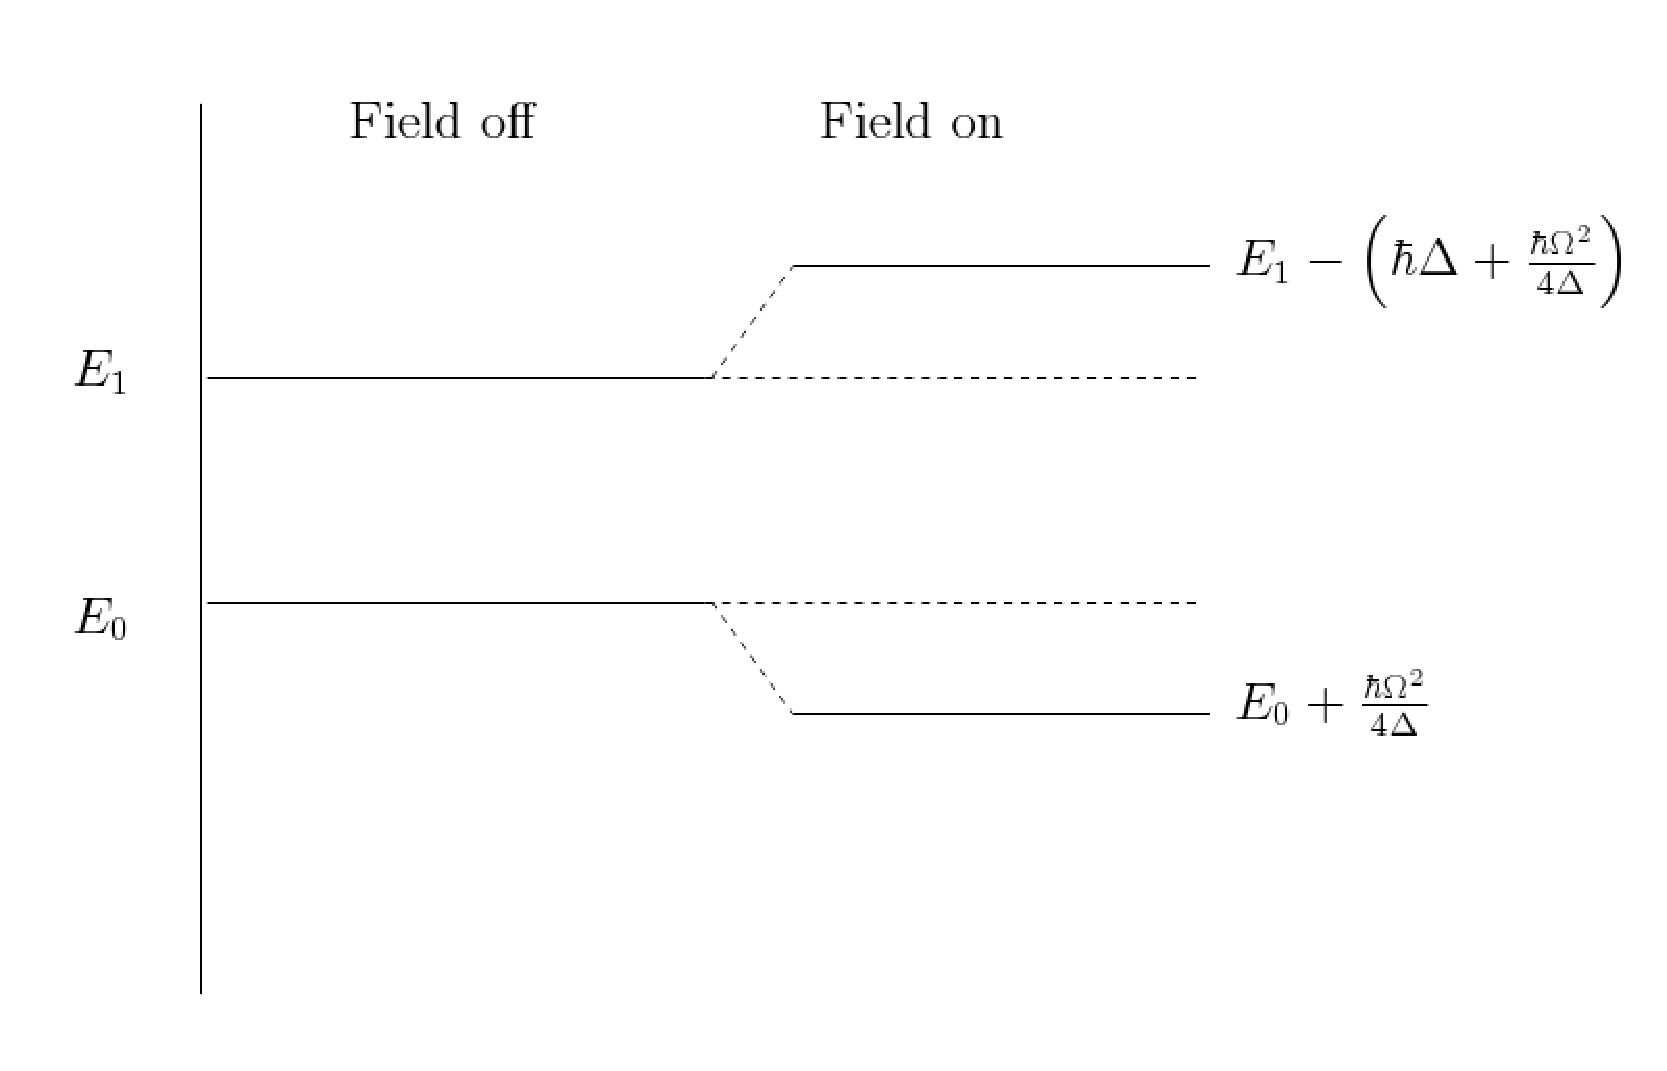
\psfig{file=jpegs/chapter-intro/fig1.eps,height=3.6in,width=5.3in}
\caption{Energies for the two-level problem with the laser field turned off and then on with negative detuning. The energy levels $E_0$ and $E_1$ are shifted due to the interaction between the system and the laser field.}
\label{fig:dressed:states:chapter-intro}
\end{figure}
Plugging these into Eqn~\ref{eq:2level:dynamics:chapter-intro} gives us (after dropping the primes)
\begin{eqnarray}
i\hbar \frac{d}{dt}\langle 0|\psi\rangle = \left( \frac{P^2}{2M} + E_0 \right) \langle 0|\psi\rangle + \frac{\hbar \Omega}{2} \langle 1|\psi\rangle S(t), \nonumber \\
i\hbar \frac{d}{dt}\langle 1|\psi\rangle = \left( \frac{P^2}{2M} + E_1 \right) \langle 1|\psi\rangle - \hbar \Delta \langle 1|\psi\rangle + \frac{\hbar\Omega}{2}\langle 0|\psi\rangle S^*(t), \nonumber \\
S(t)= e^{-i\Delta t} \left[ e^{i \left( kz-\omega t \right)}+  e^{-i \left( kz-\omega t \right)} \right] e^{-i\omega_0 t}.
\label{eq:2level:transformed:chapter-intro}
\end{eqnarray}
We now apply the R.W.A. to $S(t)$, and all the time dependent terms average out, leaving only the $z$-dependent terms, which can be treated as unity, giving us
\begin{eqnarray}
i\hbar \frac{d}{dt}\langle 0|\psi\rangle = \left( \frac{P^2}{2M} + E_0 \right) \langle 0|\psi\rangle + \frac{\hbar \Omega}{2} \langle 1|\psi\rangle, \nonumber \\
i\hbar \frac{d}{dt}\langle 1|\psi\rangle = \left( \frac{P^2}{2M} + E_1 \right) \langle 1|\psi\rangle - \hbar \Delta \langle 1|\psi\rangle + \frac{\hbar\Omega}{2}\langle 0|\psi\rangle.
\label{eq:2level:transformed:rwa:chapter-intro}
\end{eqnarray}
This is the Schr\"odinger dynamics of an effective time independent Hamiltonian $H_{eff}$ which is given by 
\begin{equation}
H_{eff} = \frac{P^2}{2M}+
\left( \begin{array}{cc}
E_0 & 0\\
0 & E_1
\end{array}
\right) + \frac{\hbar}{2} \left( \begin{array}{cc}
0 & \Omega \\
\Omega & -2 \Delta
\end{array}
\right).
\label{eq:3lvl:hamilt:chapter-intro}
\end{equation}
The energy eigenvalues are given by 
\begin{equation}
E'_{0,1}=\frac{P^2}{2M}+E_{0,1}+ \frac{\hbar}{2} \left( -\Delta \pm \sqrt{\Omega^2 + \Delta^2} \right).
\label{eq:diag:chapter-intro}
\end{equation}
The eigenvectors, $|\psi'_0 \rangle$ and $|\psi'_1 \rangle$, are referred to as 'dressed states'. The eigenvector corresponding to $E'_0$ is 
\begin{equation}
|\psi'_0 \rangle = \langle 0 | \psi \rangle \left( \begin{array}{c}
                                                 1 \\
						 W(\Omega/\Delta)
                                                \end{array}\right),
\end{equation}
where
\begin{equation}
W\left(\Omega/\Delta\right) \equiv \frac{-1+\sqrt{1+\left( \Omega/\Delta \right)^2}} {\Omega/\Delta}.
\label{eq:w:chapter-intro} 
\end{equation}
If the detuning $\Delta$ is large enough compared to $\Omega$, we can neglect $W$ 
\footnote{$\lim_{x \to 0}W(x)=0$ by l'H\^{o}pital's rule} and 'adiabatically eliminate' the excited state~\cite{graham}, yielding the eigenstate as just the ground state $\langle 0|\psi\rangle$. Thus, the excited state is eliminated and the system remains in the ground state with an effective Hamiltonian given by $E'_0$ in Eqn~\ref{eq:diag:chapter-intro} for the external degrees of freedom, ie
\begin{equation}
H_{eff}=E'_0=\frac{P^2}{2M}+E_0+ \frac{\hbar}{2} \left( -\Delta + \sqrt{\Omega^2 + \Delta^2} \right).
\label{eq:effham:chapter-intro}
\end{equation}
In the limit where $\Omega \ll |\Delta|$, we can simplify $E'_0$ by binomial approximation applied to Eqn~\ref{eq:effham:chapter-intro}.  This yields the 'Reduced Atom' Hamiltonian
\begin{equation}
H_{red}=\frac{P^2}{2M}+E_0+\frac{\hbar \Omega^2}{4\Delta},
\label{eq:redhamilt:chapter-intro}
\end{equation}
where
\begin{equation}
\delta E _0 = \frac{\hbar \Omega^2}{4\Delta},
\label{eq:starkshifts:chapter-intro}
\end{equation}
is the A.C stark shift~\cite{metcalf:vanderstraten}, and $E'_0=E_0 + \delta E_0$. 

From Eqn~\ref{eq:rabifreq:chapter-intro}, we see that the Rabi frequency $\Omega$ follows the same profile as the electric field. Therefore $\Omega^2$ follows the intensity profile of the laser in the space where the atom(s) are unconfined. A spatially inhomogeneous light field varying adiabatically in space, will thus produce a dressed state potential profile $V(x) =  \frac{ \hbar \Omega^2(x)}{4\Delta}$, the upper term of Eqn~\ref{eq:starkshifts:chapter-intro} (See Fig~\ref{fig:dressed:states:chapter-intro}). Here, the spatial variation of the electric field in $x$ produces spatial variations in $\Omega$. The resultant effective Hamiltonian, simplified from Eqn~\ref{eq:2lvl:hamilt:chapter-intro} to Eqn~\ref{eq:redhamilt:chapter-intro}, describes the translational motion of the atoms and is called the 'Reduced Atom' Hamiltonian
\begin{equation}
H_{red}(x) = \frac{P^2}{2M} + E_0 + V(x).
\end{equation}
The force resulting from the gradient is called the dipole force. If the beam intensity profile is tempered, and if $\Delta<0$, the dipole force is responsible for trapping the atoms around the maxima of the intensity profile of the laser in a particular direction. Double well potentials can be generated by bringing two laser beams with Gaussian intensity cross sections close together~\cite{dudarev:entanglement}. Standing waves produced by such lasers in counter propagating directions will produce spatially periodic optical lattice potentials~\cite{Deutsch:Jessen}~\cite{oplattice:bloch}. We will deal with both systems in this dissertation. Henceforth, all Hamiltonians in this dissertation will be presented in reduced atom form unless otherwise stated. 

To get an idea of the experimental parameters, we look at  $^{85}$Rb  atoms subjected to laser light. The electron configuration for Rubidium is $[Kr] 5s^1$. Thus, the angular momentum of the outermost electron $L=0$, and, with spin $S=1/2$ and spin-orbit coupling producing vector angular momenta ${\bf J}={\bf L}+{\bf S}$~\cite{rbdata}, we have $ J=1/2$ from the Clebsch-Gordan coefficients~\cite{sakurai}. Following the standard $^{2S+1}L_J$ convention used in atomic physics to denote $LS$ coupled orbitals, the lowest such orbital for  $^{85}$Rb is $5$ $^2S_{1/2}$. The next levels are $5$ $^2P_{1/2}$ and $5$ $^2P_{3/2}$. The transitions between these states are denoted by the $D_1$ ($5$ $^2S_{1/2}$ $\leftrightarrow$ $5$ $^2P_{1/2}$) and $D_2$ ($5$ $^2S_{1/2}$ $\leftrightarrow$ $5$ $^2P_{3/2} $) lines. 

Hyperfine structure is generated by the coupling between this angular momentum and the nuclear angular momentum ${\bf I}$, where $I=5/2$ for  $^{85}$Rb~\cite{rbdata}. We denote this total angular momentum by ${\bf F}={\bf J}+{\bf I}$. Using the Clebsch-Gordan coefficients, we get $ |J-I| \leq F \leq J+I$~\cite{sakurai}. Thus, for the $^{85}$Rb ground state, $5 ^2S_{1/2}$, we get the allowed values of $F=\left[ 2,3\right]$. For the $D_1$, excited state, $F=\left[2,3\right]$, and $F=\left[1,2,3,4 \right]$ for the $D_2$ excited state. The hyperfine splitting is calculated from the Hamiltonian given in~\cite{rbdata} and the $D_2$ levels shown in Fig~\ref{fig:rblevels}. We detune away from this resonance of $\simeq 1.6$ $eV$ which will require a red laser of about $780.241$ $nm$ (this line is more relevant than the $D_1$ line on account of its cycling transition being the one used for cooling and trapping the atom~\cite{rbdata}). The dipole matrix element is of the order of  $er_0$ where $r_0$ is the Bohr Radius~\cite{rbdata}. From Eqn~\ref{eq:rabifreq:chapter-intro}, we get $\hbar \Omega\simeq \alpha E_0$ where $\alpha\equiv e r_0 \simeq 10^{-28}$ $Cm$. Typical laser beams of power $\simeq 10 mW$~\cite{raizen} with $1/e^2$ area~\cite{encyclopedia:laser} of $\simeq 200\pi$ $(\mu m)^2$~\cite{raizen} gives us an energy flux $S\simeq 1.6 {\times} 10^{-2}$ $\frac{mW}{(\mu m)^2}$. Using the relation $S=\epsilon_0 c E^2_0$~\cite{jackson}, we get $E_0\simeq 10^5$ in SI units. Thus, $\hbar\Omega\simeq 5$ $\mu eV$, which is significantly smaller than typical detunings of $\hbar \Delta \simeq 0.1$ $meV$~\cite{steck}. Thus, reduced atom Hamiltonians are realized. Keeping the system at integer momentum $F=2$ means that the system is bosonic. Thus, a many-body system of such atoms will require boson statistics.

\begin{figure}
\hspace*{-0.1in}
\ 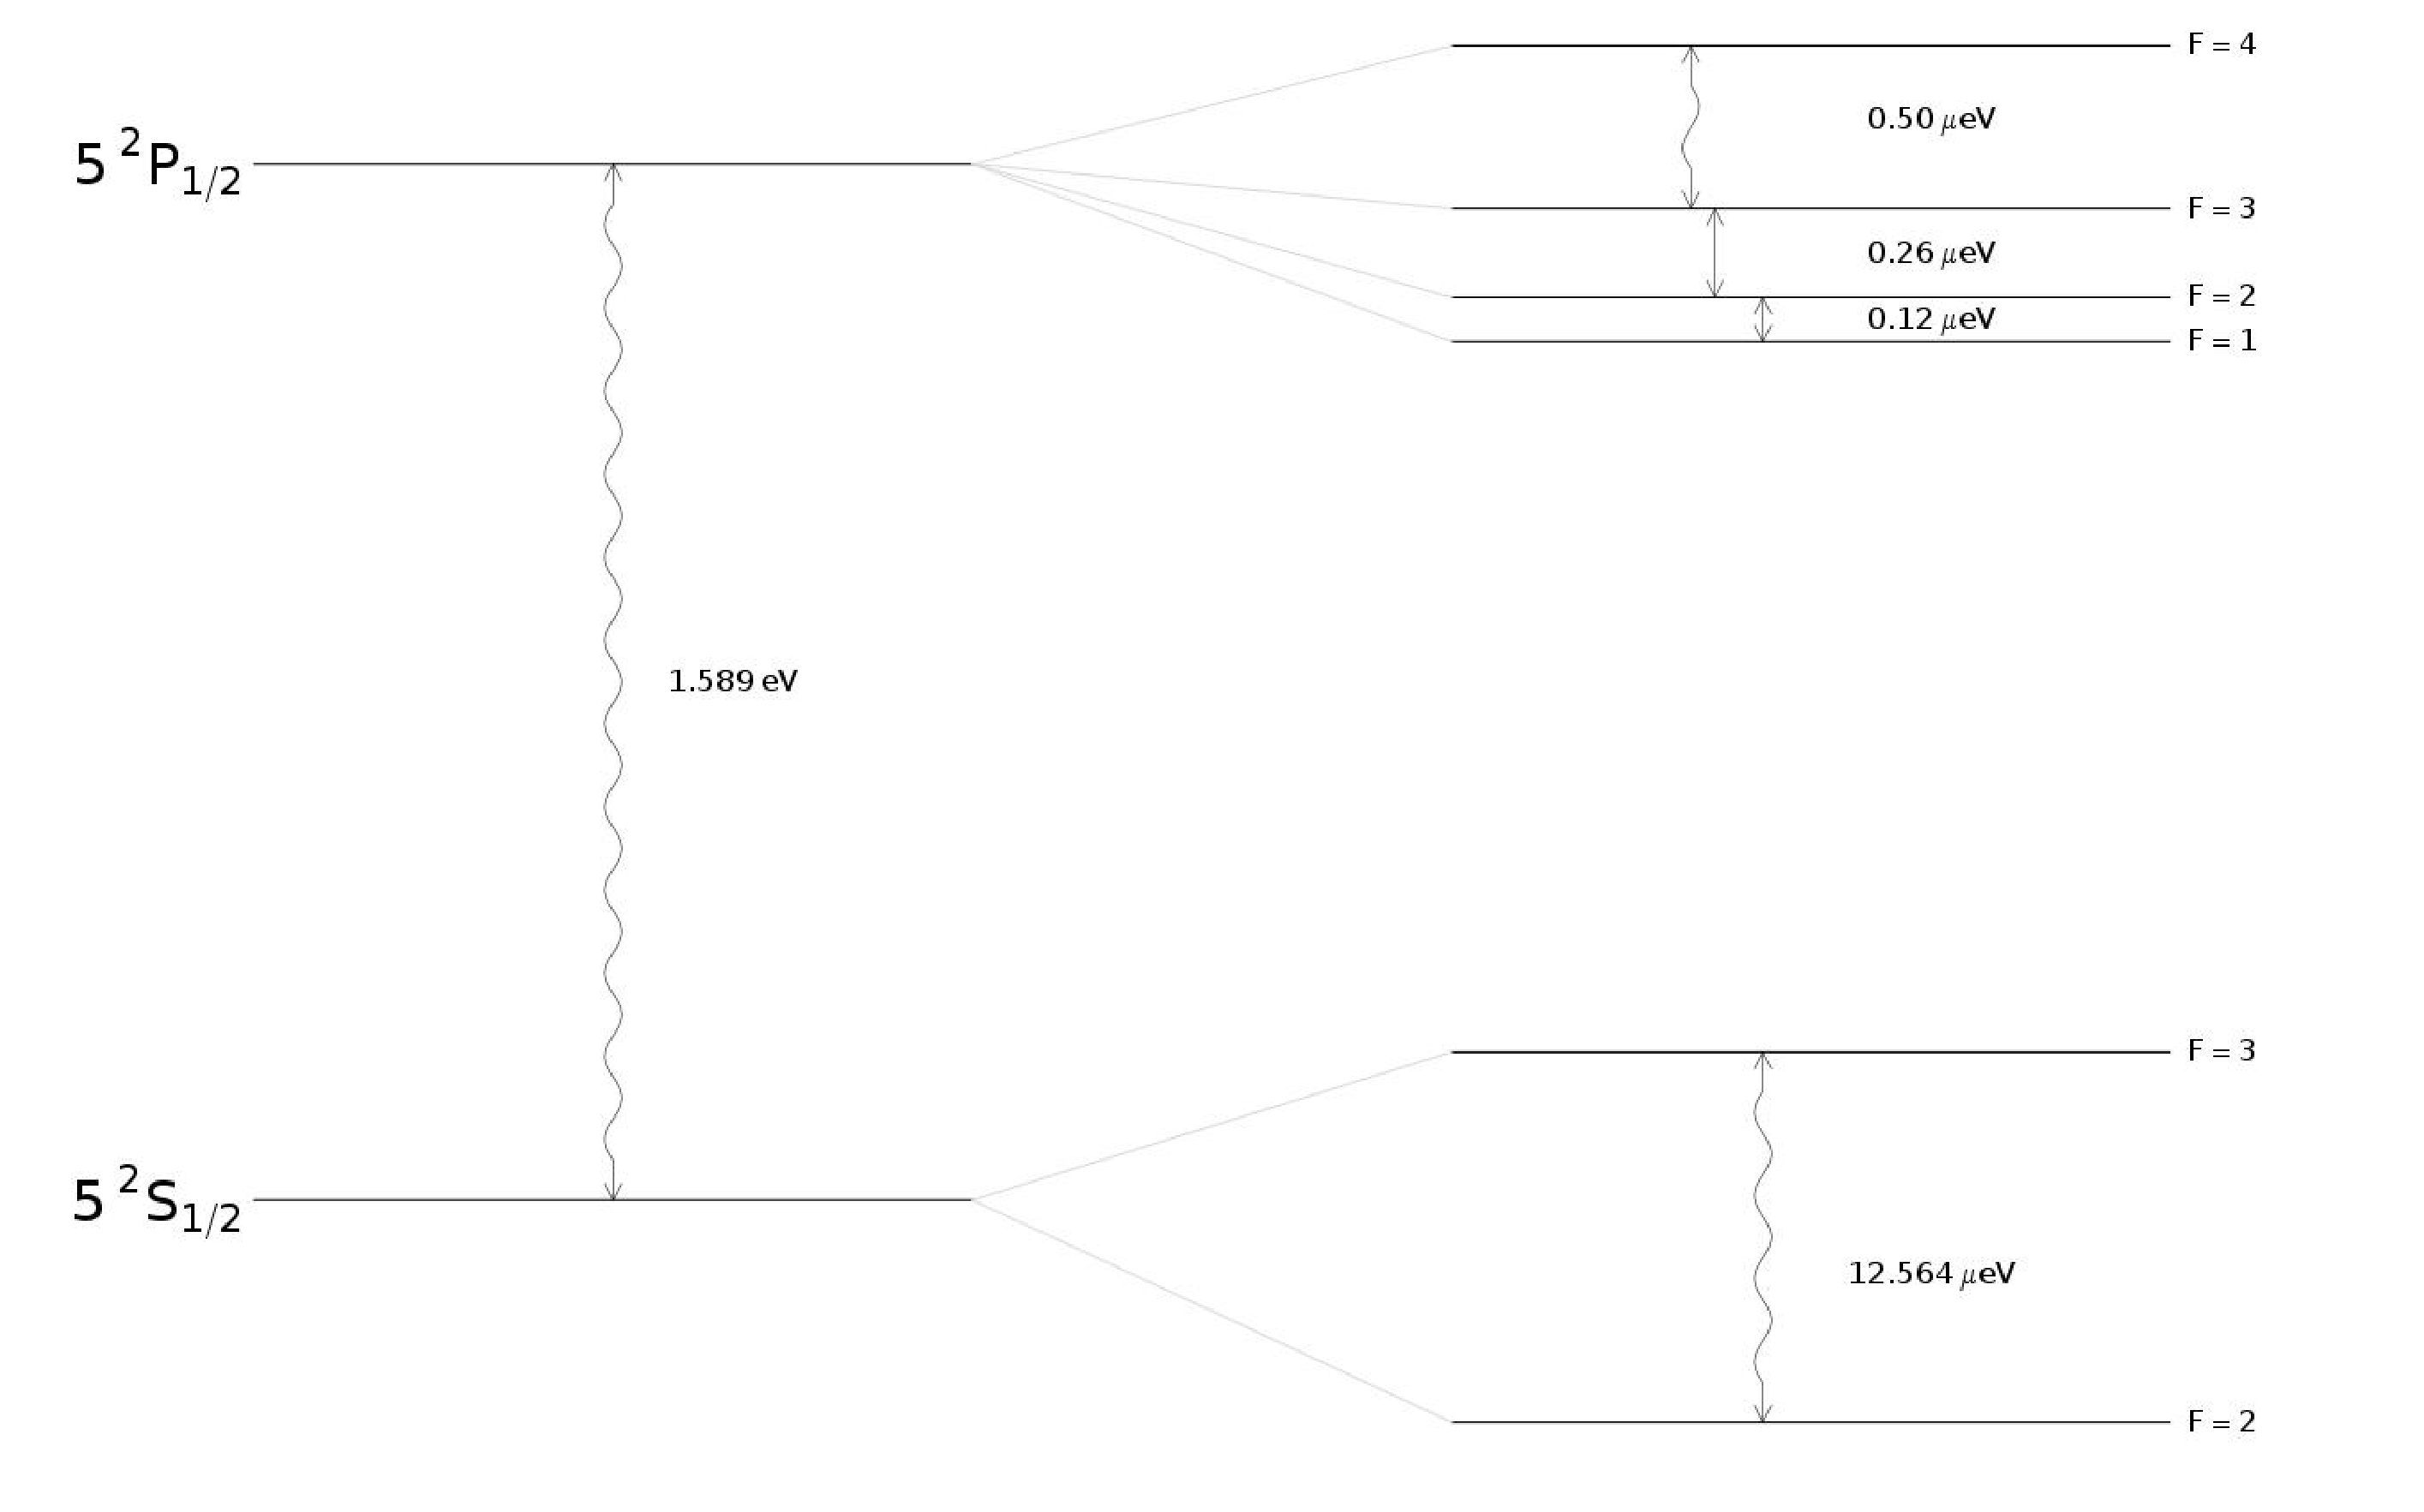
\psfig{file=jpegs/chapter-intro/fig_rblevels.eps,height=5.0in,width=5.9in}
\caption{Energy levels for the $D_2$ transition lines of  $^{85}$Rb }
\label{fig:rblevels}
\end{figure}

\subsection{Magnetic Confinement and Atom Chips}
\label{chapter-intro:section:atomchip:subsec:2lvl}
We can infer from the section above that a laser beam with a Gaussian cross section, once diffracted into two beams by diffraction methods, can be used to generate a double well system whose well separation is of the order of the wavelength of light used ($\simeq 1000$ $nm$). Sub-wavelength separations are not possible as diffraction effects will merge the double wells. For smaller length scales, we will have to exploit the dipole interactions with strong magnetic fields in atomic systems. Quadrupole magnetic fields can create zones where the magnitude of the field is a local minimum, thereby trapping the atoms, and a homogeneous RF oscillator producing a time dependent magnetic field breaks the rotational symmetry that produces the double well. These systems have been generated in the laboratory using atom chips for the purposes of matter interferometry~\cite{doublewell:chip}~\cite{doublewell:chip:nature}. Therefore, a discussion of these systems and the confinement produced by them is warranted.

Magnetic trapping of neutral atoms occurs due to the Zeeman effect, which cause the degeneracy in the hyperfine manifolds to split. For a $^{85}Rb$ atom, we have seen how the hyperfine levels $F$ are obtained from the spin-orbit-nuclear coupling (see section~\ref{chapter-intro:section:lightatom:subsec:2lvl} and~\cite{rbdata}). When an external magnetic field ${\bf B}$ is applied, the Hamiltonian describing the atomic interaction with the magnetic field is given by
\begin{eqnarray}
H=\frac{\mu_B}{\hbar} \left( g_S {\bf S}+g_L{\bf L}+g_I{\bf I}\right) \bullet {\bf B}, \nonumber \\
  = \frac{\mu_B}{\hbar} \left( g_S  S_z+g_L  L_z+g_I I_z\right)  B_z.
\end{eqnarray}
Here, the quantities $g_{(L,S,I)}$ are the Lande g-factors for the orbital, spin and nuclear angular momenta respectively, $\mu_B $ is the Bohr magneton, and the magnetic field is chosen to be in the $z-$direction. The g-factors $g_L\simeq1$, $g_s\simeq 2$, and $g_I\simeq -0.0003$~\cite{rbdata}. If the energy shift due to the magnetic field is small compared to the fine, and hyperfine splitting, then ${\bf F}={\bf L}+{\bf S}+{\bf I}$ is a 'good quantum number' and the Hamiltonian simplifies~\cite{rbdata} to
\begin{equation}
H = \mu_B g_F B_z,
\end{equation}
where
\begin{multline}
g_F \simeq \frac{F(F+1)-I(I+1)+J(J+1)}{2F(F+1)} \\
  \left\{1+ \frac{J(J+1)+S(S+1)-L(L+1)}{2J(J+1)}  \right\}.
\end{multline}
  As detailed in section~\ref{chapter-intro:section:lightatom:subsec:2lvl}, $F=2$, $L=0$, $I=5/2$, and $J=S=1/2$ for the $5$ $^2S_{1/2}$ state of $^{85}Rb$, thus $g_F\simeq-1/3$. For weak magnetic fields, $H$ perturbs the zero-field eigenstates of the hyperfine manifold. Thus, first order perturbation theory gives us~\cite{sakurai} energy shifts
\begin{equation}
\Delta E_{F,m_F} = \mu_B g_F m_F B_z ,
\label{eq:atomic:levels:chapter-intro}
\end{equation}
where $m_F$ are integers in the range $\left[-F, F \right]$. If the magnetic field is spatially varying, we now have the initial Hamiltonian for our system~\cite{lesanovsky:maghamilt}
\begin{equation}
H_{init}(t) = g_F \mu_B {\bf B}({\bf r},t) \bullet {\bf F}.
\label{maghamilt:chapter-intro}
\end{equation}
Equation~\ref{maghamilt:chapter-intro} represents the most general Hamiltonian of neutral atoms in magnetic fields. Now, the magnetic field is split into two terms,
\begin{equation}
{\bf B}({\bf r},t) =  {\bf B}_s({\bf r}) + {\bf B}_{rf}({\bf r},t).
\end{equation}
Here, ${\bf B}_s({\bf r})$ is a field that generates an Ioffe-Pritchard trap~\cite{pethick:bec}~\cite{Pritchard:trapgradients} with a global minimum in $|{\bf B}|$ at ${\bf r}=0$, and ${\bf B}_{rf}({\bf r},t)$ is a radio-frequency field that is linearly polarized in the $x-$direction. Thus,
\begin{eqnarray}
  {\bf B}_s({\bf r}) = Gx {\bf e}_x   -Gy {\bf e}_y   +B_I{\bf e}_z, \nonumber \\ 
 {\bf B}_{rf}({\bf r},t) = \frac{B_{rf}}{2}\left( e^{i\omega t}+ e^{-i\omega t} \right) {\bf e}_x,
 \label{eq:magfields:chapter-intro}
\end{eqnarray}
with $G$ being the gradient of the Ioffe field. The Hamiltonian in Eqn~\ref{maghamilt:chapter-intro} is now split up into two parts,
\begin{eqnarray}
H_{init}(t) = H_s + H_{rf}(t), \nonumber \\
H_s =  g_F \mu_B {\bf B}_s({\bf r}) \bullet {\bf F}, \nonumber \\
H_{rf}(t) = g_F \mu_B {\bf B}_{rf}({\bf r},t) \bullet {\bf F}.
\label{maghamilt:split:chapter-intro}
\end{eqnarray}
The Schr\"odinger equation for this system can be written as 
\begin{equation}
\left( H_s + H_{rf}(t) - i\hbar \frac{\partial}{\partial t} \right) |\psi(t)\rangle = 0.
\label{maghamiltdyn:split:chapter-intro}
\end{equation}
We transform each parts of Eqn~\ref{maghamiltdyn:split:chapter-intro} to a basis where $H_s$ is diagonal. If the transformation matrix is denoted by $U_s$, then
\begin{eqnarray}
U_s = \exp{\left( iF_z \phi \right)}\exp{\left( iF_y\beta\right)}, \nonumber \\
\cos{\beta} = \frac{B_I}{|{\bf B}_s({\bf r})|}, \nonumber \\
\sin{\beta} = - \frac{G\rho}{|{\bf B}_s({\bf r})|},
\label{eq:beta:chapter-intro}
\end{eqnarray}
where we have used cylindrical polar coordinates $\left[ x, y, z \right]=\left[ \rho \cos{\phi}, \rho \sin{\phi}, z \right]$. After applying the transformation, $H'_s=U^\dagger_s H_s U_s$ simplifies to 
\begin{equation}
H'_s = |{\bf B}_s({\bf r})|F_z,
\label{eq:hstrans:chapter-intro}
\end{equation}
and $H'_{rf}=U^\dagger_{rf} H U_s$. Thus, 
\begin{equation}
\left( H'_s + H'_{rf}(t) - i\hbar \frac{\partial}{\partial t} \right) |\psi(t)\rangle = 0.
\label{maghamiltdyntrans:split:chapter-intro}
\end{equation}
We proceed from here by first simplifying $H'_s$. We do so by applying a second transformation $U_r$ that rotates the system to the phase of the radio-frequency field. Thus, $U_r = \exp{\left(-i\frac{g_F}{|g_F|} F_z \omega t \right)}$, and the transformed Hamiltonian $H''_s$ is given by
\begin{equation}
H''_s - i\hbar \left( \frac{\partial}{\partial t} \right)'' =U^\dagger_r H'_s U_r - i\hbar U^\dagger_r \frac{\partial}{\partial t} U_r.
\end{equation}
Upon applying this transformation, we get
\begin{equation}
H''_s - i\hbar \left( \frac{\partial}{\partial t} \right)'' = \left( g_F  \mu_B |{\bf B}_s({\bf r})| -\frac{g_F}{|g_F|} \hbar \omega   \right).
\label{eq:hstransfinal:chapter-intro}
\end{equation}
Now, we apply all of the above transformations to $H_{rf}$. Thus, we get $H''_{rf}(t) = U^\dagger_r H'_{rf}(t)U_r$, where
\begin{multline}
H''_{rf}(t) =   \frac{g_F \mu_B B_{rf}}{2}\left( e^{i\omega t}+ e^{-i\omega t} \right) \times   \\
\exp{\left(i\frac{g_F}{|g_F|} F_z \omega t \right)} \exp{\left(- iF_y\beta\right)}  \exp{\left(- iF_z \phi \right)} \times \\
   F_x   \exp{\left( iF_z \phi \right)}\exp{\left( iF_y\beta\right)}  \exp{\left(-i\frac{g_F}{|g_F|} F_z \omega t \right)}.
\end{multline}
This equation can be evaluated by applying the Baker-Campbell-Hausdorff formula on each pair of exponentials on either side of $F_x$~\cite{sakurai}, and simplifying the expansion using the angular momentum commutation relations $\left[ F_i, F_j \right] = i\hbar \epsilon_{ijk} F_k$ (where the square bracket indicates $\left[ F_i, F_j \right] \equiv F_iF_j-F_jF_i$, and $\epsilon_{ijk}$ is the Levi-Civita symbol). After applying the rotated wave approximation (RWA) and neglecting terms that oscillate with frequency of $2\omega$ or higher (cf section~\ref{chapter-intro:section:lightatom:subsec:2lvl}), we get 
\begin{eqnarray}
H''_{rf}(t) = \frac{g_F \mu_B}{2} \bar{{\bf B}} \bullet {\bf F}, \nonumber \\
\bar{{\bf B}} = B_{rf} \left( \cos{\beta} {\bf e}_x + \sin{\phi}\sin{\beta}{\bf e}_y \right).
\label{eq:hrftransfinal:chapter-intro}
\end{eqnarray}
We now obtain an expression for the rotated wave Hamiltonian $H''$ for the whole system by applying Eqns~\ref{eq:hstransfinal:chapter-intro} and~\ref{eq:hrftransfinal:chapter-intro} to Eqn~\ref{maghamiltdyn:split:chapter-intro}. After dropping the primes, this gives us (for the LHS of Eqn~\ref{maghamiltdyn:split:chapter-intro})
\begin{equation}
H= \left( g_F  \mu_B |{\bf B}_s({\bf r})| -\frac{g_F}{|g_F|} \hbar \omega   \right) + \frac{g_F \mu_B}{2} \left(\bar{B}_x F_x + \bar{B}_y F_y  \right).
\label{maghamilt:rwa:chapter-intro}
\end{equation}
Thus, the solution to the dynamics of Eqn~\ref{maghamiltdyn:split:chapter-intro} can be reduced to diagonalizing the time independent rotated wave Hamiltonian $H$. This can be done in the $m_F$ representation by writing out the matrix elements using the ladder     
operator relations for the angular momentum ${\bf F}$~\cite{sakurai}. We now diagonalize this Hamiltonian in a two level system similar to the one in section~\ref{chapter-intro:section:lightatom:subsec:2lvl}, where we select two consecutive $m_F$ states. The adiabatic potential thus obtained is~\cite{lesanovsky:maghamilt}
\begin{equation}
V({\bf r}) = g_F m_F \mu_B \sqrt{\left( |{\bf B}_s({\bf r})|-\frac{\hbar \omega}{|g_F \mu_B|} \right)^2+ \frac{1}{4} \left( \bar{B}_x^2 + \bar{B}_y^2 \right)}.
\end{equation}
This can be simplified in cylindrical polar coordinates $\left[\rho, \phi \right]$ by using the definitions in Eqns~\ref{eq:beta:chapter-intro} and~\ref{eq:hrftransfinal:chapter-intro} to yield
\begin{equation}
V({\bf r}) = g_F m_F \mu_B \sqrt{\left[ |{\bf B}_s({\bf r})|-\frac{\hbar \omega}{|g_F \mu_B|} \right]^2 + \left[\frac{B_{rf}}{2|{\bf B}_s({\bf r})|} \right]^2 \left( B^2_I +G^2 \rho^2 \sin^2\theta \right)}.
\end{equation}
The minima of this potential can be found at $\theta = \left[0, \pi \right]$ (provided that $g_F m_F >0$). If the radius $\rho \ll B_I/G$, we can approximate
\begin{eqnarray}
V(\rho) \simeq g_F m_F \mu_B \sqrt{\frac{G^4}{B^2_I}\left(\frac{\rho^2-\rho^2_0}{2} \right)^2+B^2_0}, \nonumber \\
\rho^2_0 \equiv \frac{B^2_{rf}-B^2_c}{2G}, \nonumber \\
B_0 \equiv \frac{B_{rf}}{4B_I}\sqrt{4B^2_I + B^2_C -2 G^2\rho^2_0}, \nonumber \\
B_c \equiv 2\sqrt{B_I \left( \frac{g_F\mu_B B_I -\hbar\omega}{|g_F\mu_B|}\right)}.
\label{eq:magpot:chapter-intro}
\end{eqnarray}
From Eqns~\ref{eq:magpot:chapter-intro}, we can clearly see that the potential $V(\rho)$ is a one-dimensional double well potential along the polar direction of the 
the potential minima. The well minima can be found at $\rho=\pm \rho_0$ about the origin. Transforming to the $\theta= 0$ or $\pi$ axis, we get 
\begin{equation}
V(x) = g_F m_F \mu_B \sqrt{\frac{G^4}{B^2_I}\left(\frac{x^2-x^2_0}{2} \right)^2+B^2_0}.
\label{eq:1dmagpot:chapter-intro}
\end{equation}
where $x_0=\rho_0$. For a sufficiently high Ioffe field $B_I$ , $\left(G^2x^2_0/2B_I\right) \ll B_0$~\cite{pethick:bec}~\cite{doublewell:chip}, and Eqn~\ref{eq:1dmagpot:chapter-intro} can be expanded binomially to get an equation of the type
\begin{equation}
 V(x)= V_0 (-2{\bar x}^2 + {\bar x}^4),
\end{equation}
where we have dropped overall constant terms, and defined
\begin{eqnarray}
 V_0 \equiv \frac{g_F m_F \mu_B G^4 x^4_0}{8B_0B^2_I}, \nonumber \\
 {\bar x}\equiv \frac{x}{x_0}. 
 \label{eq:welldepth:chapter-intro}
 \end{eqnarray}
Note that ${\bar x}$ is dimensionless, and $V_0$, which gives us the well-depth, has the dimensions of energy. Thus, after adding the translational degrees of freedom ($\frac{p^2}{2m}$) to the above simplification of the atomic interaction with the magnetic field, we can get a 'reduced atom' Hamiltonian of a particle in a quartic double well whose minima can be found at $\pm x_0$. 

Such potentials have been achieved with atom chip systems by Schumm et al in 2006~\cite{doublewell:chip}~\cite{doublewell:chip:nature}. In these experiments, an atom chip containing lithographically etched DC current-carrying micro-wires (which, when combined with an external pair of Helmholtz coils, generates the quadrupole field for an Ioffe-Pritchard trap~\cite{pethick:bec}) together with a micro-wire carrying an ac current (for the RF field), confines a BEC in a double well potential immediately below the chip. The radio frequencies of about $500$ $KHz$ and magnetic fields $B_{rf}\equiv 1$ Gauss in a standard Ioffe-Pritchard trap. We note that, from Eqn.~\ref{eq:magpot:chapter-intro}, $x_0=\sqrt{\left(B_{rf}^2-B^2_c\right)/2G}$. The parameters in the double well atom chip of Schumm et al produce an $x_0$ of the order of $10$ $\mu m$. If we desire a well-separation of $L_u=50$ $nm$, and a potential well depth ($V_{max}(x)$ of Eqn~\ref{eq:1dmagpot:chapter-intro}) that is of the order of $E_u=\frac{\hbar^2}{2mL_u^2}$ for the mass $m$ of a $^{85}Rb$ atom, then we need to solve the simultaneous equations
\begin{eqnarray}
V_0=E_u \nonumber \\
x_0=L_u.
\label{eq:magpot:roots:chapter-intro}
\end{eqnarray}
Using Eqns~\ref{eq:welldepth:chapter-intro} and~\ref{eq:magpot:chapter-intro}, we get
\begin{eqnarray}
\frac{g_Fm_F\mu_BG^4x^4_0}{8B_0B^2_I}=E_u=\frac{\hbar^2}{2mL^2_u} \nonumber \\
\frac{B^2_{rf}-B^2_c}{2G} = L^2_u,
\label{eq:magtrap:roots:chapter-intro}
\end{eqnarray}
where $B_0$ and $B_c$ are obtained from Eqns~\ref{eq:magpot:chapter-intro}. Equation~\ref{eq:magtrap:roots:chapter-intro} need to be solved for a given $L_u$, which we desire to be around $50$ $nm$, and for experimentally feasible parameters for the Ioffe-Pritchard trap. We choose to solve for the radial trap gradient $G$ and RF frequency $\omega$, with Ioffe Field $B_I=100$ $Gauss$ and RF field amplitude $B_{rf}=1$ $Gauss$ (both values are typical for this system~\cite{Pritchard:trapgradients}~\cite{doublewell:chip}). Figure~\ref{fig:magplots:chapter-intro} shows the progression towards the solution with graphs, where $V_0/E_u$ and $x_0/L_u$ are plotted as functions of $\omega$ for several values of $G$, ranging from $1$ $T/m$ to $10,000$ $T/m$ or $100$ $T/cm$. The intersection of the two graphs approaches unity in the latter most case, the exact solution for $G$ being $11303.375$ $T/m$ at $\omega=292.955314305$ $MHz$ (see Fig~\ref{fig:magplots:chapter-intro}.d). Radial field gradients much higher than this magnitude ($10^5$ $T/m$) have been reported for micro-magnets generated by wires lithographically etched on chips~\cite{drndic:higrad}~\cite{lev:highgrad}. Thus, one can readily obtain a stable double well system for the $F=2$, $m_F=-2$ state of $^{85}Rb$ within the required parameters. 
\begin{figure}
\ \psfig{file=jpegs/chapter-intro/fig_magplots.eps,height=5.2in,width=5.5in}
\caption{Graphical representation of the numerical solution to Eqn~\ref{eq:magpot:roots:chapter-intro} or~\ref{eq:magtrap:roots:chapter-intro}. Figures (a) through (d) plot dimensionless functions $V_0/E_u$ and $x_0/L_u$ as functions of the RF frequency $\omega$ for radial gradients $G=1$, $10$, $1000$ and $10^4$ $T/m$ respectively. The Ioffe Field $B_I=100$ $Gauss$ and RF field amplitude $B_{rf}=1$ $Gauss$. Both curves must intersect at unity for a solution, and Fig (d) shows plots for  the closest value of $G$ for which this happens (unity is indicated by a horizontal line). Fine-tuning the bisection method gives us the more accurate solution of $G=11303.375$ $T/m$ for $\omega=292.955314305$ $MHz$.}
\label{fig:magplots:chapter-intro}
\end{figure}
\section{Avoided Crossings and the Landau Zener Formula}
\label{chapter-intro:section:avcross}
An introduction to the concept of avoided crossings is provided here. We consider a quantum system described by a finite-dimensional Hilbert space $\cal H$. The Hamiltonian $H(\lambda)$ is parametrized by $\lambda$. The  'No-Crossing theorem' by von-Neumann and Wigner establishes that the variation of a single parameter in a finite-dimensional, 'general' Hermitian matrix ( a matrix with no relations between the matrix elements other than Hermiticity) cannot produce degeneracies in the eigenvalue spectrum. Thus, if symmetries (such as parity) exist, then eigenvalues may cross each other freely as the parameter is varied~\cite{vonneumann:wigner}. The symmetries cause eigenvalues to 'cross' each other in the parameter space, and breaking the symmetry causes those crossings to 'avoid' each other (see Fig~\ref{fig:2lvl:avcross:chapter-intro}), producing an 'avoided crossing' at that point. For a simple two level system similar to the one discussed in the last section, we have
\begin{equation}
H_0(\lambda)= \lambda \left( |0\rangle \langle 0| - |1\rangle \langle 1| \right),
\label{eq:hamilt:avcross:chapter-intro}
\end{equation}
where we have scaled our zero level for the energy to be midway between the unperturbed energies of the Hamiltonian. We apply a 'perturbation' $H'$ to this Hamiltonian, with the system now described by 
\begin{eqnarray}
H=H_0(\lambda)+H'(\delta), \nonumber \\
H'(\delta) = \delta \left( |0\rangle \langle 1| + |1\rangle \langle 0| \right),
\end{eqnarray}
or
\begin{equation}
H = \left( \begin{array}{cc}
            \lambda & \delta\\
	    \delta & -\lambda
           \end{array}\right).
\label{eq:fullhamilt:avcross:chapter-intro}
\end{equation}
\begin{figure}
\ 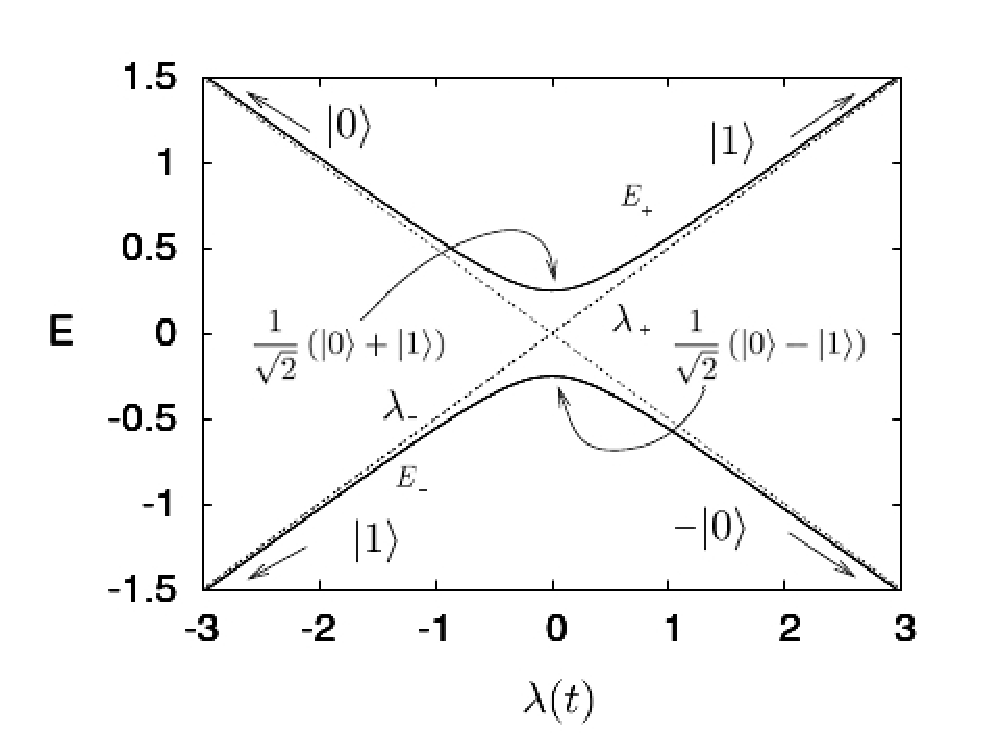
\psfig{file=jpegs/chapter-intro/fig_avcross.eps,height=3.0in,width=4.0in}
\caption{Adiabatic and diabatic eigenvalue curves of the 2 level quantum system. The diabatic ($\delta=0$) eigenvalues, $\lambda\pm$, are shown as dashed lines, and the adiabatic curves, $E_\pm$ are shown as solid curves (for $\delta=0.5$). Arrows indicate eigenstate character in the diabatic $\left[|0\rangle, |1\rangle \right]$ representation.}
\label{fig:2lvl:avcross:chapter-intro}
\end{figure}
The energy eigenvalues of this system are
\begin{equation}
E_\pm = \pm \sqrt{\lambda^2 + \delta^2},
\label{eq:2lvlen:chapter-intro}
\end{equation}
and are plotted in Fig~\ref{fig:2lvl:avcross:chapter-intro}. as a function of $\lambda$. They approach each other and 'avoid' a crossing at $\lambda=0$ by a factor of $2\delta$. We diagonalize the general Hamiltonian using the diagonal basis for $\lambda=0$. Thus, denoting the eigenstates as $| \lambda_\pm \rangle$, we have
\begin{equation}
| \lambda_\pm \rangle = C^0_\pm | (\lambda=0)_- \rangle + C^1_\pm | (\lambda=0)_+ \rangle,
\end{equation}
where 
\begin{equation}
| (\lambda=0)_\pm \rangle = \frac{1}{\sqrt{2}} \left( |0\rangle \pm |1\rangle \right).
\label{eq:avcross2lvl:chapter-intro}
\end{equation}
This Hamiltonian is transformed to the $|(\lambda=0)_\pm \rangle$ basis by $H^t(\lambda) = S^\dagger H(\lambda) S$, where
\begin{equation}
 S = \left(\begin{array}{cc}
        1 &1 \\
	-1 & 1
       \end{array}\right),
\end{equation}
yielding 
\begin{equation}
 H^t(\lambda)=\left(\begin{array}{cc}
                     \delta & -\lambda \\
		     -\lambda & -\delta
                    \end{array}\right),
\end{equation}
with the same eigenvalues. Solving for the $|\lambda_\pm \rangle$ eigenvectors, we get 
\begin{equation}
\frac{ C^0_\pm}{ C^1_\pm} = \frac{\lambda}{\delta \mp \sqrt{\lambda^2 + \delta^2}}.
\end{equation}
Now, we note the following limits for the ratio of the components of the eigenvector(s) viz.
\begin{equation}
\lim_{\lambda \to -\infty}\frac{ C^0_\pm}{ C^1_\pm} = \pm 1,
\label{eq:limits1:chapter-intro} 
\end{equation}
and
\begin{equation}
\lim_{\lambda \to +\infty}\frac{ C^0_\pm}{ C^1_\pm} = \mp 1 .
\label{eq:limits2:chapter-intro} 
\end{equation}
Thus, we see from Eqns~\ref{eq:limits1:chapter-intro} and ~\ref{eq:limits2:chapter-intro} that a state populated at $|0\rangle$ at $\lambda=-\infty$ will change character and switch over to $|1\rangle$ as the system adiabatically crosses $\lambda=0$ and approaches $\lambda=\infty$ and vice versa. Similarly, a state populated at $|1\rangle$ at $\lambda=-\infty$ will change character and switch over to $-|0\rangle$ as the system adiabatically crosses $\lambda=0$ and approaches $\lambda=\infty$ and vice versa. At $\lambda=0$, the states are given by Eqn~\ref{eq:avcross2lvl:chapter-intro}, and are thus 'mixed' between the two canonical basis states. 

This phenomenon is called an 'avoided crossing' and will be pivotal to our understanding of the full many-level dynamics of quantum control. The dynamics of a quantum controlled STIRAP will be described by a parameter $t_{fix}$ which will vary adiabatically, analogous to $\lambda$ in this section. The loss of symmetry will produce avoided crossings for particular values of $t_{fix}$ in the same region that the corresponding system loses the same symmetry (ie it is not integrable). The absence of invariant tori in the $\left[J, \Theta \right]$ space, a consequence of classical non integrability, causes the dynamics to transition to chaos in these regimes~\cite{reichl}. Thus, the presence of these avoided crossings and their effect on the spectral statistics on the system is a quantum manifestation of classical chaos, and their study merits interest in that context.

So far, we have ignored any temporal dependence in the variation of $\lambda$. We have implicitly relied on the fact that the quantum adiabatic theorem, first obtained by Max Born and Vladamir Fock in 1928, guarantees that a physical system remains in its instantaneous eigenstate if a given perturbation is acting on it slowly enough and if there is a gap between the eigenvalue and the rest of the Hamiltonian's spectrum~\cite{Born1928:adiabaticthm}. However, a distinction must be made between an \textit{adiabatic process}, where gradually changing conditions allow the system to adapt its configuration, hence modifying the probability density, and a \textit{diabatic process},  where rapidly changing conditions prevent the system from adapting its configuration during the process~\cite{kato:adiabaticthm}. In an adiabatic process, if the system starts in an eigenstate of the Hamiltonian, it will end in the corresponding eigenstate of the final Hamiltonian after a long time, changing character through any avoided crossings on the way in order to remain in it's adiabatic eigenvalue curve (in this case, $E_\pm$). However, this mechanism is disturbed if the parameters do not vary adiabatically. In such a case, the actual state of the system projects into other eigenstates of the Hamiltonian, causing the system to lose coherence~\footnote{In the extreme case of a diabatic process,  it's the probability density that remains unchanged. The system ends in a linear combination of states that sum to reproduce the initial probability density}. Thus, there is no eigenstate of the final Hamiltonian with the same functional form as the initial state~\cite{kato:adiabaticthm}. 

The criterion for a system to evolve adiabatically depends on several factors, such as the time scale $\tau$ for the variation of $\lambda$, as well as the energy gap between the eigenstate and the rest of the spectrum. For a two-level quantum system such as this, the Landau-Zener formula is an analytical solution that gives the probability of a diabatic transition between the two energy states. It was published separately by Lev Landau~\cite{landau:lzformula} and Clarence Zener~\cite{zener:lzformula} in 1932. Among the numerous derivations that have been published since then, we present a short summary of an elegant derivation of this relation by Wittig~\cite{wittig:lzformula}. If we plug in a time dependence on $\lambda$, and assume that the system starts at $t=-\infty$ in the lower energy eigenstate $|\lambda_-\rangle$, we can calculate the probability of finding the system in the upper energy eigenstate $|\lambda_+\rangle$ at $t=\infty$.  In order that the equations of motion for the system might be solved analytically, a set of simplifications are made, known collectively as the Landau-Zener approximation. The simplifications are as follows:
\begin{itemize}
 \item 
 The perturbation parameter in the Hamiltonian is a known, linear function of time, making this treatment semiclassical.
 \item
 The energy separation of the diabatic states varies linearly with time ie $\lambda(t)=\frac{\Gamma}{2} t$, where $2 \lambda$ is the energy level difference from Eqn.~\ref{eq:hamilt:avcross:chapter-intro}. Thus, $\Gamma$ is the rate at which the diabatic energy levels $\pm \lambda$ approach each other at the avoided crossing at $t=0$.
 \item
 The coupling in the diabatic Hamiltonian matrix is independent of time, ie $\delta$ is constant.
\end{itemize}

We now integrate the system in the canonical diabatic basis ($|0\rangle$, $|1\rangle$, which are the eigenstates for the diabatic case of $\delta=0$) by writing the state vector as
\begin{equation}
|\psi(t)\rangle = A(t) |0\rangle e^{-i\int^t dt' \lambda(t')} + B(t) |1\rangle e^{i\int^t dt' \lambda(t')}.
\end{equation}
Here, $\hbar=1$. Applying the Schr\"odinger equation $H|\psi(t)\rangle=i\frac{d}{dt}|\psi(t)\rangle$ for the Hamiltonian in Eqn.~\ref{eq:fullhamilt:avcross:chapter-intro}, and resolving the components in the diabatic basis, we get (in the interaction picture)
\begin{eqnarray}
\dot{A} = -i \delta B e^{2i\int^t dt' \lambda(t')}, \nonumber \\
\dot{B} = -i \delta A e^{-2i\int^t dt' \lambda(t')}.
\end{eqnarray}
Differentiating the above with respect to time and simplifying leads to
\begin{eqnarray}
\ddot{A} -2i\lambda(t) \dot{A} + \delta^2 A=0, \nonumber \\
\ddot{B} +2i\lambda(t) \dot{B} + \delta^2 B=0.
\end{eqnarray}
We now apply the itemized assumptions above and write out the equation for $B(t)$, getting
\begin{equation}
\ddot{B} + i\Gamma t \dot{B} + \delta^2 B=0.
\label{eq:eqn4B:chapter-intro}
\end{equation}
Here, $B(t)$ is the amplitude of the wavefunction in the 'excited state' $|1\rangle$. We desire to obtain an expression for $B(\infty)$, which will give us the probability of the system being measured at the excited state long after the avoided crossing at $t=0$ has been encountered. Assuming that $B(t)$ is nonvanishing for all finite times~\cite{wittig:lzformula}, we divide Eqn~\ref{eq:eqn4B:chapter-intro} by $dt/(Bt)$ and integrate over all times to get
\begin{equation}
i\Gamma \int^{B(\infty)}_1 \frac{dB}{B} = - \delta^2 \int^\infty_{-\infty} \frac{dt}{t} - \int^\infty_{-\infty} \left( \frac{dt}{t} \frac{\ddot{B}(t)}{B(t)}\right).
\label{eq:toint:chapter-intro}
\end{equation}
The limits of integration for $B$ are decided by the state populating the lower eigencurve of Fig~\ref{fig:2lvl:avcross:chapter-intro}. at $t=-\infty$, which has the characteristic of $|1\rangle$, making $B(-\infty)=1$. The first term in the RHS of Eqn~\ref{eq:toint:chapter-intro} can be integrated by the calculus of residues~\cite{arfken}. Thus,
\begin{eqnarray}
\int^\infty_{-\infty} \frac{dt}{t} = \lim_{\epsilon \to 0} \left( \int^\epsilon_{-\infty} + \int_\epsilon^\infty \right) \frac{dt}{t}, \nonumber \\
  = \left(\oint_C - \oint_{C_1}\right) \frac{dt}{t}.
\label{eq:int1:chapter-intro}
\end{eqnarray}
Here, the contours $C$ and $C_1$ are shown in Fig~\ref{fig:contours:chapter-intro}, and the sense of the integration indicated by arrows. The limit $\epsilon \rightarrow 0$ is implicit in the second equation. In the limit $R \rightarrow \infty$, Jordan's Lemma causes the $C$- contour integral to vanish~\cite{arfken}. In the contour $C_1$, $t=\epsilon e^{i\theta}$ with constant $\epsilon$. Thus, substitution into the contour integral gives $i\pi$, and Eqn~\ref{eq:toint:chapter-intro} simplifies to
\begin{equation}
\ln B(\infty) = - \pi \delta \tau - i \frac{\tau}{\delta}\int^\infty_{-\infty} \left( \frac{dt}{t} \frac{\ddot{B}(t)}{B(t)}\right),
\label{eq:eqn4lnB:chapter-intro}
\end{equation}
where $\tau=-\delta/\Gamma$. 

We now analytically continue the function $\frac{\ddot{B}(t)}{B(t)}$ into the complex plane~\cite{wittig:lzformula} and evaluate the integral. Evaluating the integral above  using the calculus of residues along the same contours as shown in Fig~\ref{fig:contours:chapter-intro} gives us
\begin{equation}
 \int^\infty_{-\infty} \left( \frac{dt}{t} \frac{\ddot{B}(t)}{B(t)}\right) =i \lim_{\epsilon \to 0} \int^0_\pi d\theta \frac{\ddot{B}(\epsilon)}{B(\epsilon)} + \lim_{R \to \infty} \int^\pi_0 i d\Theta \frac{\ddot{B}(R)}{B(R)}.
 \end{equation}
Note that the expression $\frac{\ddot{B}(t)}{B(t)}$ has no phase dependencies~\cite{wittig:lzformula}. Thus, taking the limits causes both integrals in the RHS to vanish, and Eqn~\ref{eq:eqn4lnB:chapter-intro} simplifies to 
\begin{eqnarray}
\ln B(\infty) = -\pi \delta \tau, \nonumber \\
B(\infty) = e^{-\pi \delta \tau}.
\end{eqnarray}
Finally, the probability $P_{10}$ that the state will be found in $|1\rangle$ is given by $|B(\infty)|^2$, ie
\begin{equation}
P_{10}=e^{-2\pi \delta \tau}.
\end{equation}
We now have an expression that will help us in determining the time scale for adiabatic dynamics for this system. If $\delta \tau \gg 1/2\pi$, the probability $P_{10}$ is negligible, and the system is found in state $|0 \rangle$ at $t=\infty$, avoiding the crossing at $t=0$ completely. If $\delta \tau \ll 1/2\pi$, $P_{10} \simeq 1$ and the state crosses the avoided crossing at $t=0$, causing it to not change character and remain in $|1\rangle$ at $t=\infty$. Recall that the energy gap at $t=0$ is $2 \delta$ (see Eqn~\ref{eq:2lvlen:chapter-intro}), and $\tau=-\delta/\Gamma$. Noting that $\Gamma$, the approach velocity, is negative in this case, we have
\begin{equation}
P_{10}=\exp{\left[ -2\pi\frac{\delta^2}{|\Gamma|}\right]}.
\label{eq:lzformula:chapter-intro}
\end{equation}
The approach velocity $\Gamma=|\frac{d\lambda_+}{dt}-\frac{d\lambda_-}{dt}|_a$, where the derivatives are the slopes of the asymptotes of the adiabatic eigenvalues near the avoided crossing (the diabatic energies). Equation~\ref{eq:lzformula:chapter-intro} is called the 'Landau-Zener formula', and will be used in later sections to approximately obtain time scales for adiabaticity in STIRAP processes in multilevel systems.
\begin{figure}
\ 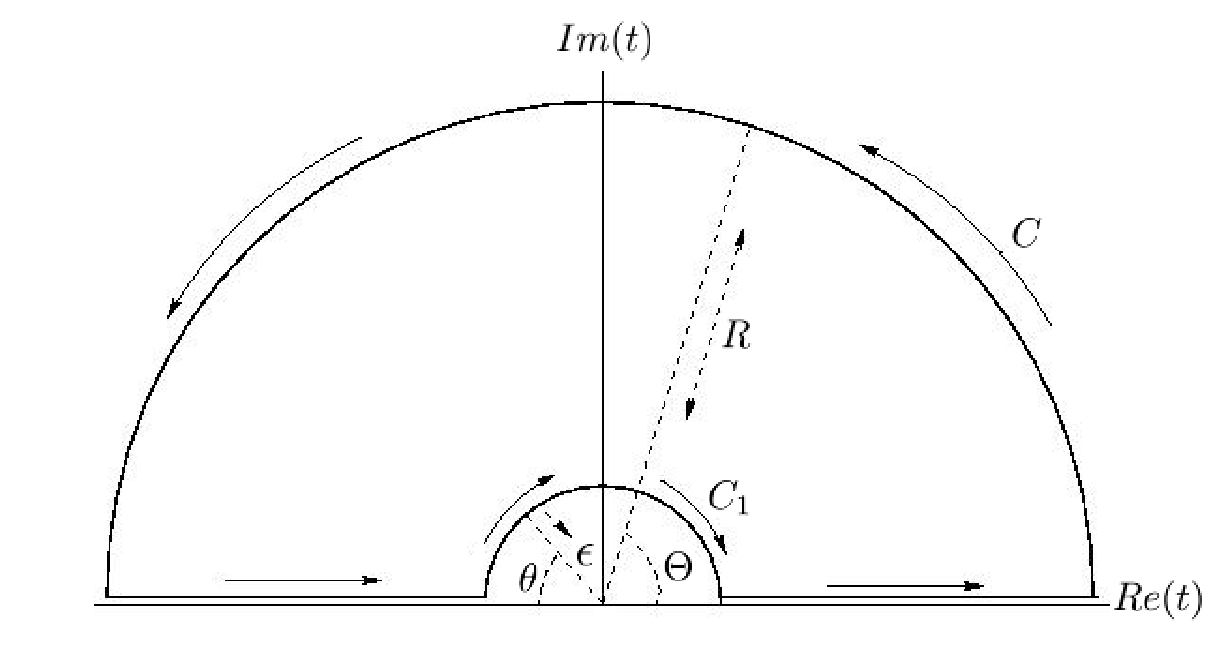
\psfig{file=jpegs/chapter-intro/fig_contours.eps,height=3.0in,width=5.0in}
\caption{Contours chosen for the integrals in Eqns~\ref{eq:int1:chapter-intro} and~\ref{eq:eqn4lnB:chapter-intro} in the complex plane. The radius $R \rightarrow \infty$ is the radius of the contour $C$, and the radius $\epsilon \rightarrow 0$ is the radius of the contour $C_1$. The angles of a particular point on $C$ and $C_1$ are denoted by $\Theta$ and $\theta$ respectively.}
\label{fig:contours:chapter-intro}
\end{figure}

\section{Three Level STIRAP}
\label{chapter-intro:section:stirap}
Stimulated Raman Adiabatic Passage, or STIRAP,  is a well-known method of inducing coherent excitations of quantum systems from the ground state to states with higher energy. This is achieved using coherent time-modulated laser fields that result in complete population transfer from an initially populated ground state to a target state via an intermediate state (see Fig~\ref{fig:3lvl:stirap:chapter-intro}). STIRAP was first proposed by Hioe and coworkers~\cite{stirap:hioe}~\cite{hioe:rwa:stirap}.  A crucial preliminary work by Becker, Gaubatz, Jones and Bergmann that achieved efficient vibrational excitation by using the molecular beam as an optically pumped active medium in a laser, led to the development of the STIRAP concept~\cite{stirap:seminal}. The theoretical work was formulated by Kuklinsky, Gaubatz, Hioe and Bergmann shortly thereafter~\cite{stirap:theory}. STIRAP was further confirmed by manipulating the vibrational and rotational degrees of freedom in sodium dimers~\cite{stirap:experiment}. Since then, STIRAP has been used to understand a diverse range of matter-optics systems, ranging from molecular alignment~\cite{stirap:molecular}, and molecular rotation~\cite{na-reichl:mol-rot}, to the coherent acceleration of ultracold atom systems~\cite{holder:reichl:2res}. This dissertation analyzes chaos in the latter for interacting bosons. In this section, we will be looking at the dynamics of STIRAP for a simple three level system. In further chapters, we will be investigating the effects of deterministic chaos in this dynamics by analyzing the STIRAP dynamics of the full multilevel system. 
\begin{figure}
\ 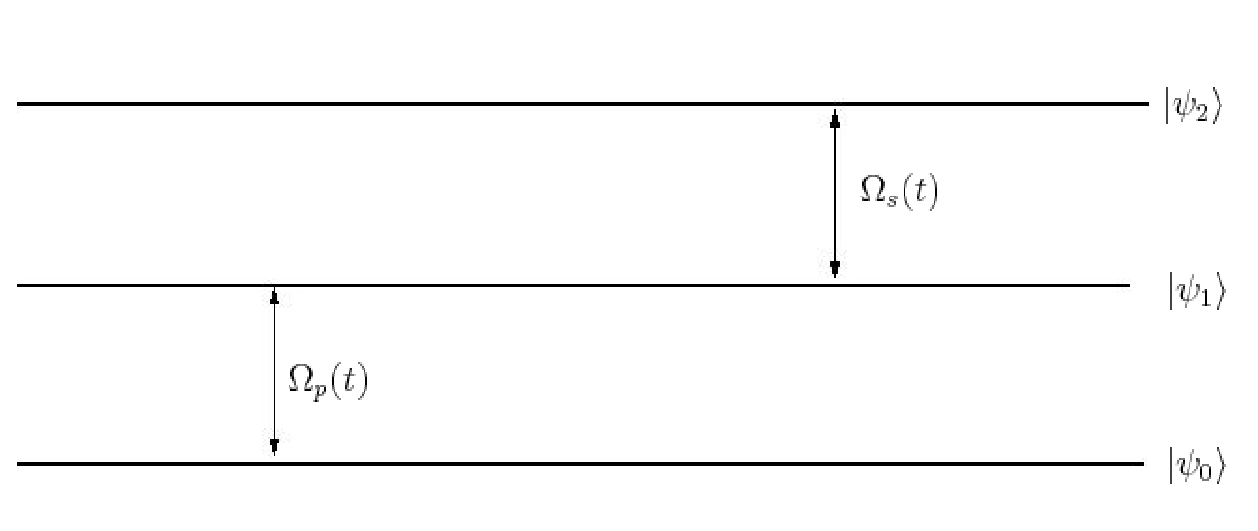
\psfig{file=jpegs/chapter-intro/fig_stirap.eps,height=3.0in,width=5.0in}
\caption{Linkage diagram for a three level Stimulated Raman Adiabatic Passage (STIRAP). A pump field of Rabi frequency $\Omega_p(t)$ and a Stoke field of Rabi frequency $\Omega_s(t)$ couple the states $\left \vert \psi_0\rangle , \vert \psi_1\rangle \right]$ and $\left[ \vert \psi_1\rangle, \vert \psi_2\rangle \right]$ respectively (as indicated by double arrows). If the Stoke field is switched on before the pump field, then the system, initially populated at $\vert \psi_0\rangle$, will achieve a complete population transfer to $\vert \psi_2\rangle$. The detunings $\Delta_{p,s}$ have been set to $0$.}
\label{fig:3lvl:stirap:chapter-intro}
\end{figure}
\subsection{Adiabatic time evolution}
For this simple three-level system, we denote the initial populated state at $t=-\infty$ by $|\psi_0\rangle$, the target state by $|\psi_2\rangle$, and the intermediate state by $|\psi_1\rangle$. The states  $|\psi_0\rangle$ and  $|\psi_1\rangle$ will be connected by a 'pump pulse' (of detuning $\Delta_p=0$), and the states  $|\psi_1\rangle$ and  $|\psi_2\rangle$ by a 'Stoke pulse' (of detuning $\Delta_s=0$). Figure~\ref{fig:3lvl:stirap:chapter-intro} illustrates the process with a linkage diagram for no detuning.
These pulses will have amplitudes that vary slowly in time from zero, to a peak value, then back to zero ('switching on' and then 'switching off'). Unlike other methods of excitations like optical pumping, this will be a two-photon resonance, similar to stimulated emission pumping, and the Stoke pulse will be switched on before the pump pulse.~\cite{stirap:hioe}~\cite{stirap:theory}~\cite{stirap:review}. Applying the R.W.A to this three-level system simplifies the Hamiltonian~\cite{hioe:rwa:stirap} to
\begin{equation}
H(t)=\hbar \left(
\begin{array}{ccc}
0 & \frac{1}{2}\Omega_p(t) & 0 \\
 \frac{1}{2}\Omega_p(t) & \Delta  & \frac{1}{2}\Omega_s(t)\\
 0 &  \frac{1}{2}\Omega_s(t) & 0
\end{array}
\right),
\label{eq:3lvl:stirap:hamilt:chapter-intro}
\end{equation}
where  $\Omega_{p,s}$  are the Rabi frequencies for the pump and Stoke pulses respectively, and describe the temporal profile of the switches (see Eqn~\ref{eq:rabifreq:chapter-intro}). Also, $\Delta=\Delta_p=\Delta_s$ is the single photon detuning of both pulses (necessarily kept equal). 

In the $\left[ |\psi_0\rangle, |\psi_1\rangle, |\psi_2\rangle  \right]$ basis, the adiabatic eigenvalues and eigenstates can be obtained by simply diagonalizing this Hamiltonian. The adiabatic eigenvalues of this Hamiltonian are
\begin{eqnarray}
\epsilon_0(t)=0, \nonumber \\
\epsilon_{\pm}(t) = \frac{1}{2}\left[ \Delta \pm \sqrt{\Delta^2 + \Omega'^2(t)}\right]. 
\label{eq:3lvl:evals:chapter-intro}
\end{eqnarray}
Solving the equations $H |\Phi_{0,\pm}\rangle = \epsilon_{0,\pm} |\Phi_{0,\pm}\rangle$ gives us
\begin{eqnarray}
|\Phi_+(t)\rangle = |\psi_0\rangle \sin{\theta(t)}\sin{\phi(t)} + |\psi_1\rangle \cos{\phi(t)}+|\psi_2\rangle \cos{\theta(t)}\sin{\phi(t)}, \nonumber \\
|\Phi_0(t)\rangle=|\psi_0\rangle \cos{\theta(t)} -|\psi_2\rangle \sin{\theta(t)}, \nonumber \\
|\Phi_-(t)\rangle = |\psi_0\rangle \sin{\theta(t)}\cos{\phi(t)} + |\psi_1\rangle \sin{\phi(t)}+|\psi_2\rangle \cos{\theta(t)}\cos{\phi(t)}.
\label{eq:3lvl:stirap:estates:chapter-intro}
\end{eqnarray}
Here, the mixing angles $\theta(t)$ and $\phi(t)$ are defined as
\begin{eqnarray}
\theta(t) \equiv \arctan{\frac{\Omega_p(t)}{\Omega_s(t)}}, \nonumber \\
\phi(t) \equiv \frac{1}{2} \arctan{\frac{\Omega'(t)}{\Delta}},
\label{eq:3lvl:mixang:chapter-intro}
\end{eqnarray}
and 
\begin{equation}
\Omega'(t)\equiv \sqrt{\Omega^2_p(t) + \Omega^2_s(t)}.
\label{eq:3lvl:omegap:chapter-intro}
\end{equation}
The state $|\Phi_0(t)\rangle$ has components only in the $\left[ |\psi_0\rangle , |\psi_2\rangle \right]$ subspace and no component in $|\psi_1\rangle$ and so is a trapped 'dark' state~\cite{stirap:review}. Thus, if we arrange it so that $\sin{\theta(t)}$ vanishes as $t \rightarrow -\infty$, and $\cos{\theta(t)}$ vanishes as $t \rightarrow \infty$, then $|\Phi_0\rangle$ will go from fully populating $|\psi_0\rangle$ to $|\psi_2\rangle$ as time evolves. From Eqns~\ref{eq:3lvl:mixang:chapter-intro}, we see that this is only possible if the mixing angle $\theta$ rises from $0$ to $\pi/2$ as time passes, meaning that the Rabi frequency and hence the amplitude (see Eqn~\ref{eq:rabifreq:chapter-intro}) of the Stoke pulse, $\Omega_s(t)$ must exceed that of the pump pulse, $\Omega_p(t)$ at earlier times. Therefore, the pulses must be applied in the counterintuitive 'Stoke first' order as described above for a complete population transfer to take place.

Figure~\ref{fig:evol:chapter-intro}.a through Fig~\ref{fig:evol:chapter-intro}.c shows plots for the system as it evolves through the STIRAP process in time $t$ (expressed in units of $t_{tot}$) with  $\Delta=0$. Figure~\ref{fig:evol:chapter-intro}.a shows plots for the Rabi frequencies $\Omega_p(t)$ and $\Omega_s(t)$, where the time dependence is chosen to be Gaussian ie $\Omega_{p,s}(t)=\Omega_0 e^{-(t-t_{p,s})^2/(2t^2_d)}$, with $t_s<t_p$. Thus, the Stoke pulse is 'switched on' before the pump pulse in the counterintuitive order. Figure~\ref{fig:evol:chapter-intro}.b shows the time evolution of the adiabatic eigenstates $\epsilon_{0,\pm}$ from Eqn~\ref{eq:3lvl:evals:chapter-intro}. Note the three-level avoided crossing at $t=0.5$ $t_{tot}$ where the dark state $|\Phi_0\rangle$ exchanges character with a linear combination of the $|\Phi_{\pm}\rangle$ states to finally obtain the character of $|\psi_2\rangle$. This is verified by Fig~\ref{fig:evol:chapter-intro}.c. In this figure, the evolution of the dark state $|\Phi_0\rangle$ is plotted as a function of time. The probabilities $P_i = |\langle \psi_i |\Phi_0\rangle|^2$ are shown for states $|\psi_0\rangle$ and $|\psi_2\rangle$ (see Eqns~\ref{eq:3lvl:stirap:estates:chapter-intro}). The population transfer from $|\psi_0\rangle$ to $|\psi_2\rangle$ is clearly seen at $t=0.5$ $t_{tot}$.

\begin{figure}
\ \psfig{file=jpegs/chapter-intro/fig_evol.eps, height=5.2in, width=3.5in}
\caption{Time evolution of the three level STIRAP problem. Figure (a) shows the Rabi frequency plots for the pump pulse $\Omega_p$, and Stoke  pulse $\Omega_s$ (scaled 
w.r.t $\Omega_0$) as functions of time $t$. The pulses have a Gaussian time dependence, with $t_s=(1/3)$, and $t_p=(2/3)$. The pulse widths of both pulses are $t_d=(1/10)$. Figure (b) shows the time dependence on the adiabatic eigenvalues $\epsilon_{0,\pm}$ of the Hamiltonian in Eqn~\ref{eq:3lvl:stirap:hamilt:chapter-intro} (see Eqn~\ref{eq:3lvl:evals:chapter-intro}). Figure (c) shows the time evolution of the dark state $|\Phi_0\rangle$ in Eqn~\ref{eq:3lvl:stirap:estates:chapter-intro} by plotting the occupation probability $P_i$ in undriven state $|i\rangle$. At $t=0$, it starts from a fully populated ground state $|0\rangle$ and switches character midway to fully populate $|2\rangle$, thereby achieving STIRAP. In all cases, the time is expressed in arbitrary units of $t_{tot}$. the detuning $\Delta=0$}
\label{fig:evol:chapter-intro}
\end{figure}

\subsection{Adiabaticity criterion}

We note that this evolution will be followed by the system in the strictly adiabatic limit, when no diabatic transitions take place between the eigenstates on account of time dependence. Thus, the system will be temporally adiabatic enough to follow this profile if the eigenstates of Eqns~\ref{eq:3lvl:stirap:estates:chapter-intro} are orthogonal compared to the eigenvalue differences~\cite{stirap:theory}~\cite{stirap:review} ie
\begin{equation}
|\langle \frac{d\Phi_0}{dt}|\Phi_\pm\rangle| \ll |\epsilon_0-\epsilon_\pm|.
\end{equation}
Simplifying the above for $\Delta=0$ gives us
\begin{equation}
\Omega'(t)\gg |\frac{d\theta(t)}{dt}|.
\label{eq:stirap:adiabaticity:chapter-intro}
\end{equation}
We assume that the Rabi frequencies vary in time as Gaussians, ie
\begin{equation}
\Omega_{p,s}(t) = \Omega_0 e^{-\beta (t-t_{p,s})^2} ,
\end{equation}
with $t_s>t_p$ so that the stoke pulse is 'switched on' first. Plugging the above equation into From Eqns~\ref{eq:3lvl:mixang:chapter-intro} and~\ref{eq:3lvl:omegap:chapter-intro} and applying Eqn~\ref{eq:stirap:adiabaticity:chapter-intro}, we get 
\begin{equation}
\Omega_0 \gg \left( 2\beta \right) \Gamma(t, t_s, t_p, \beta),
\label{eq:inequality:chapter-intro}
\end{equation}
where
\begin{equation}
\Gamma(t,t_s, t_p, \beta) \equiv \left( t_s - t_p \right) \frac{e^{-\beta (t-t_p)^2}e^{-\beta (t-t_s)^2}}{\left[ e^{-2\beta(t-t_s)^2} + e^{-2\beta(t-t_p)^2}     \right]^{3/2}}.
\end{equation}
Now, $t_s>t_p$ for a complete population transfer. If we use a time scale for the total time for both the pulses to traverse (denoted by $t_{tot}$), and scale all the time scales in $\Gamma$ , including the pulse widths $t_d \equiv 1/(\sqrt{2\beta})$,  by $t_{tot}$, then $(t_s-t_p)<t_{tot}$. If $t<t_s$, then we can simplify $\Gamma$ to the expression below. Thus,
\begin{equation}
\Gamma(t,t_s,t_p,\beta) = \left( t_s-t_p \right) \frac{e^{-\beta (t-t_p)^2}e^{2 \beta (t-t_s)^2}}{\left[ 1 + \frac{e^{-2\beta(t-t_p)^2}}{e^{-2\beta(t-t_s)^2}}     \right]^{3/2}}<t_{tot} 
\end{equation}
if $t_d \ll t_{s,p}$. Similarly, we can interchange $t_p$ for $t_s$ in the above expression for the range $t_s<t<t_p$ and arrive at the same conclusion. A similar argument can be made for $t_p<t<t_{tot}$ as well. Thus, in general, $\Gamma<t_{tot}$ and so can be eliminated from the inequality in Eqn.~\ref{eq:inequality:chapter-intro} to get the simple result
\begin{equation}
\Omega_0 t_d \gg \frac{t_{tot}}{t_d}.
\end{equation}
Since $t_d \ll t_{tot}$, it follows that $\Omega_0 t_d \gg 1$ is sufficient for the condition above to hold. Since the area of a Gaussian pulse is of the order of $\Omega_0  (t_d/t_{tot})$, it follows that the area of the pulse should be much greater than unity for adiabaticity to hold true. This will be a significant point in later chapters where actual pulse amplitudes need to be adjusted for the double well system.

\include{chapter-dblwell}
  \chapter{Stimulated Raman Adiabatic Passage in Optical Lattices}
\index{Stimulated Raman Adiabatic Passage in Optical Lattices%
@\emph{Stimulated Raman Adiabatic Passage in Optical Lattices}}%
\label{chapter-optical_lattice}
\section{\label{sec:1} Introduction}
As we have seen for the double well case in chapter~\ref{chapter-dblwell}, avoided crossings of eigenvalue curves are an important feature of quantum systems with non-integrable classical counterparts. This was demonstrated theoretically by Von Neumann and Wigner as part of seminal work~\cite{von-Neumann:Wigner}. This phenomenon allows for many interesting phenomena related to chaos. In particular, the adiabatic exchange of character provides a mechanism by which the underlying classical chaos affects the quantum dynamics~\cite{na-reichl:pbox}~\cite{mypaper}. Their existence is responsible for the well-known phenomenon of 'quantum chaos' in the spectral statistics of the system~\cite{reichl}. In this chapter, we look at coherently controlled excitations of atoms trapped in an optical lattice via the same STIRAP technique used for the double well system in chapter~\ref{chapter-dblwell}. 

An optical lattice is a periodic potential formed by the AC Stark shift seen by atoms when they interact with interfering laser beams. The way that this potential is generated follows from the theory of light-atom interactions, and is shown in section~\ref{chapter-intro:section:lightatom}, and detailed specifically for the optical lattice in the next section. While optical lattice systems have been of great interest in experimental physics (see, for instance,~\cite{oplattice:oldexpt} and~\cite{oplattice:oldexpt2}) and theoretical physics~\cite{oplattice:oldtheory}~\cite{oplattice:oldtheory2} for some time, it was in 1992 when Graham, Schlautmann and Zoller proposed that dynamic localization of the type being discussed in this dissertation is achievable~\cite{graham}. Since then, such systems have sparked considerable experimental and theoretical interest.  The properties of ultracold atoms in optical lattices can be used to precisely control many-body systems and  function as analog quantum computers, allowing for exploration of physical regimes inaccessible in regular condensed-matter systems. This led to the discovery of groundbreaking physics in these systems, such as the famous superfluid-Mott insulator transition by Jaksch and Zoller in 1998~\cite{sfmi:theory} (later seen experimentally by Grenier, Mandel,  Esslinger, Hansch and Bloch~\cite{sfmi:expt}). The dynamics of chaos in these systems has also been the subject of attention in recent years~\cite{graham}, including chaos as reported by Graham, Schlautmann and Zoller themselves. The dynamics and the influence of chaos in such dynamics is an important factor in the manipulation of such systems~\cite{raizen:oplattice}, such as the coherent acceleration of atoms from stationary to mobile states~\cite{holder:reichl:2res}. More recently (2009), number squeezing and subpoissonian distribution of atoms in each site in an optical lattice have been reported by Itah et al that is similar to the atom culling considered for the double well in chapter~\ref{chapter-dblwell}~\cite{technion:oplattice-culling}.

The optical lattice system that we will be investigating is a two-parameter system of the harmonically driven pendulum which has been implemented in a number of experimental studies~\cite{steck}~\cite{luter:reichl:3res} through ultracold atom optical systems. In the following sections, we will study the properties of avoided crossings for the driven pendulum with the use of Floquet theory as we did for the double well system in chapter~\ref{chapter-dblwell}. We will facilitate a time dependent 'radiation pulse' by the use of multiple resonances from mobile lattices that share the same period as the stationary lattice. Avoided crossings in the Floquet states can be associated with real transitions of the undriven eigenstates, and is an indication of the influence of deterministic chaos in the quantum dynamics of this system.

\section{\label{sec:2}The Basic Model}
We saw in chapter~\ref{chapter-intro} section~\ref{chapter-intro:section:lightatom} that an atom, confined in one dimension, it's dynamics described by a single outermost electron, and subjected to a laser field far detuned from it's internal atomic resonances, can be described by a 'Reduced Atom' Hamiltonian.
\begin{equation}
H(x)=\frac{p^2}{2m}+\frac{\hbar^2 \Omega^2(x)}{4\Delta}.
\label{eq:redatom:chapter-oplattice}
\end{equation}
Here, $\Omega(x)$ is the Rabi frequency defined by Eqn~\ref{eq:rabifreq:chapter-intro}. 

Now, if the electric field is produced by $M$ lasers, all polarized in the $z$-direction, such that the $j^{th}$ laser is projected with a frequency that is slightly deviated by a factor $\left[ \frac{\delta \omega_j}{2},\frac{ \delta k_j}{2} \right]$  from a fixed $\left[ \omega,k \right]$~\footnote{The derivation shown here is based on the noninteracting case shown in~\cite{holder:thesis}}, we have
\begin{equation}
E_z(x,t) = \sum^{M}_{j=1} E^{j}_0 \exp{\left[ i \left\{ \left( k+\frac{\delta k_j}{2} \right)x + \sigma_j \left(\omega+\frac{\delta \omega_j}{2} \right)t \right\} \right]}.
\label{eq:lasers:chapter-oplattice}
\end{equation}
Here, $\sigma_j=\pm 1$ decides the direction of propagation in the $x$ direction, and $\delta \omega_j=c\delta k_j$. If $M=2$, and the two lasers are counterpropagating in the $x$ direction with the same amplitude and wavelength, Eqn~\ref{eq:lasers:chapter-oplattice} gives us $E^{Re}_z(x,t)=E_\kappa \left[ \cos{\left(kx-\omega t \right)} +\cos{\left(kx+ \omega t \right)} \right]=E_\kappa(x) \cos{\omega t}$, where $E_\kappa(x)=E_\kappa \cos{kx}$. Plugging $E_\kappa(x)$ into Eqn~\ref{eq:rabifreq:chapter-intro} and then into Eqn~\ref{eq:redatom:chapter-oplattice} gives us the Hamiltonian for this system viz.
\begin{equation}
H(x)=\frac{p^2}{2m}+\kappa \cos{\left( 2 kx \right)},
\label{eq:standingwave:chapter-oplattice}
\end{equation}
where $\kappa=\frac{\hbar^2 E^2_\kappa}{4\Delta}$. This system is a standing wave optical lattice of frequency $2 k$. Also, this system is basically just the quantum pendulum, and it's eigensystem consists of Mathieu functions and their characteristics for the energy eigenvalues~\cite{reichl}~\cite{abramowitz:stegun}. 

Now, if the two counter-propagating lasers are slightly off in their frequencies by a factor $\pm  ({\delta \omega}/2,{\delta k}/2)$, we then get a traveling electric field
\begin{multline}
E_z(x,t) =  E_\lambda  \exp{ \left[ i \left\{ \left( k-\frac{\delta k}{2} \right)x +  \left(\omega-\frac{\delta \omega}{2} \right)t \right\} \right] } \\
  +  E_\lambda \exp{\left[ i \left\{ \left( k+\frac{\delta k}{2} \right)x -  \left(\omega+\frac{\delta \omega}{2} \right)t \right\} \right]}.
\end{multline}
Taking the square of the above and neglecting the rapidly oscillating terms, we get 
\begin{equation}
E^2_z(x,t) = E^2_\lambda e^{i\left(2kx - \delta \omega t \right)}.
\end{equation}
Plugging the real part into Eqn~\ref{eq:rabifreq:chapter-intro} and then into Eqn~\ref{eq:redatom:chapter-oplattice} gives us an optical lattice traveling with speed $\delta \omega$ viz
\begin{equation}
H(x)=\frac{p^2}{2m} + \lambda \cos{\left( 2kx-\delta \omega t \right)},
\end{equation}
where $\lambda=\frac{\hbar^2 E^2_\lambda}{4\Delta}$ for the amplitude of this laser. Combining this with the standing wave configuration of lasers in Eqn~\ref{eq:standingwave:chapter-oplattice} gives us a time periodic two-resonance Hamiltonian
\begin{equation}
H_{2res}(x)=\frac{p^2}{2m} +\kappa \cos{\left( 2 kx \right)}+ \lambda \cos{\left(2kx-\delta \omega t\right)}.
\label{eq:twores:chapter-oplattice}
\end{equation}
Duplicating the same pair of lasers, but moving in the opposite direction, produces the time periodic three-resonance Hamiltonian. 
\begin{equation}
H_{3res}(x)=\frac{p^2}{2m} +\kappa \cos{\left( 2 kx \right)}+ \lambda \cos{\left( 2kx \right)}\cos{\delta \omega t}.
\label{eq:threeres:chapter-oplattice}
\end{equation}
If we subjected this system to a similar pair of frequency-offset lasers, we would get a five-resonance Hamiltonian
\begin{equation}
H_{5res}(x)=\frac{p^2}{2m} +\kappa \cos{\left( 2 kx\right) }+ \lambda \cos{\left( 2kx \right)} \cos{\delta \omega t}+\lambda' \cos{\left( 2kx \right)} \cos{\delta \omega ' t}
\label{eq:fiveres:chapter-oplattice}
\end{equation}
In the limit $\lambda, \lambda'=0$, the five resonance Hamiltonian reduces to the standing wave Hamiltonian. 

We now introduce the index $i$ to distinguish between the atoms in a two-boson system subjected to these Hamiltonians. It is also useful to write the Hamiltonians above in terms of dimensionless parameters $(p'_i, x_i',H'_i)$. We define $p'_i=\frac{p_i}{2\hbar k}$, and $x'_i=2 k x$. Thus, $H'_i=\frac{H}{4\hbar\omega_r}$, and $t'=4\omega_r t$, where $\omega_r=\frac{\hbar k^2}{2m}$ is the recoil frequency. We scale the driving frequencies(s) as $\omega'=\frac{\delta\omega}{4\omega_r}$, and then drop the primes on the dimensionless parameters, we obtain the dimensionless Hamiltonian for the standing wave system viz.
\begin{eqnarray}
H=p^2_1 + p^2_2+\kappa \cos{x_1}+\kappa \cos{x_2} + u_0 \delta(x_1-x_2),
\label{eq:hamscale:chapter-oplattice}
\end{eqnarray}
where we have introduced the point contact pseudopotential interaction $u_0 \delta(x_1-x_2)$ in the exact same way as in section~\ref{chapter-dblwell:section:basicmodel}. Similarly, dimensionless forms for the resonance Hamiltonians can be obtained in a straightforward way.

To get an idea of the experimental parameters, we look at the numbers for $^{85}Rb$ subjected to such a system as we did in chapters~\ref{chapter-intro} and~\ref{chapter-dblwell}. As shown in Fig~\ref{fig:rblevels}, the $D_2$ line is $1.5$ $eV$ in energy, and, as referred to in chapter~\ref{chapter-dblwell}, typical detunings are of the order of $0.1$ $meV$~\cite{steck}. The modulations $\delta \omega$ will be chosen to couple the energy levels of the stationary optical lattice for the purposes of STIRAP. For the $D_2$ line, the recoil frequency, $ \omega_r$ is thus about $24$ $KHz$, making the energy scale of the problem ($4 \hbar \omega_r$) equal to $0.02$ $neV$. That will be the typical modulations required to produce STIRAP.

The Hilbert space of the system can be restricted to the space of all $N$-periodic wavefunctions that are square-integrable, where $M$ an appropriate period of the lattice. Experimentally, such a system is realized on account of the momentum transfer occurring in discrete units of the optical lattice photons (unity in our dimensionless scale)~\cite{steck}~\cite{luter:reichl:3res}. Thus, the problem is reduced to a 'ringed' lattice of period $N$ (see Fig~\ref{fig:latticering:chapter-oplattice}). The eigenvalues of the single-particle momentum operator are integers $p_i|p_i\rangle=n|p_i\rangle$ ($n\epsilon Z$), where $|p_i\rangle$ are free particle states $e^{inx_i}$ normalized to within $N$ periods. The corresponding energy eigenvalues $|n_i\rangle$ are the basis states used to diagonalize the full Hamiltonian. The free particle energy eigenbasis is isomorphic to
\begin{equation}
\langle x | n \rangle=\left\{
\begin{array}{lll}
 \frac{1}{\sqrt{N\pi}}\cos{nx} & n>0 \\
 \frac{1}{\sqrt{2N\pi}} & n=0 \\
 \frac{1}{-\sqrt{N\pi}}\sin{nx } & n<0 .
\end{array}
\right.
\label{eq:freeptcl:chapter-oplattice}
\end{equation}
%Fig 1
 \begin{figure}
 \ 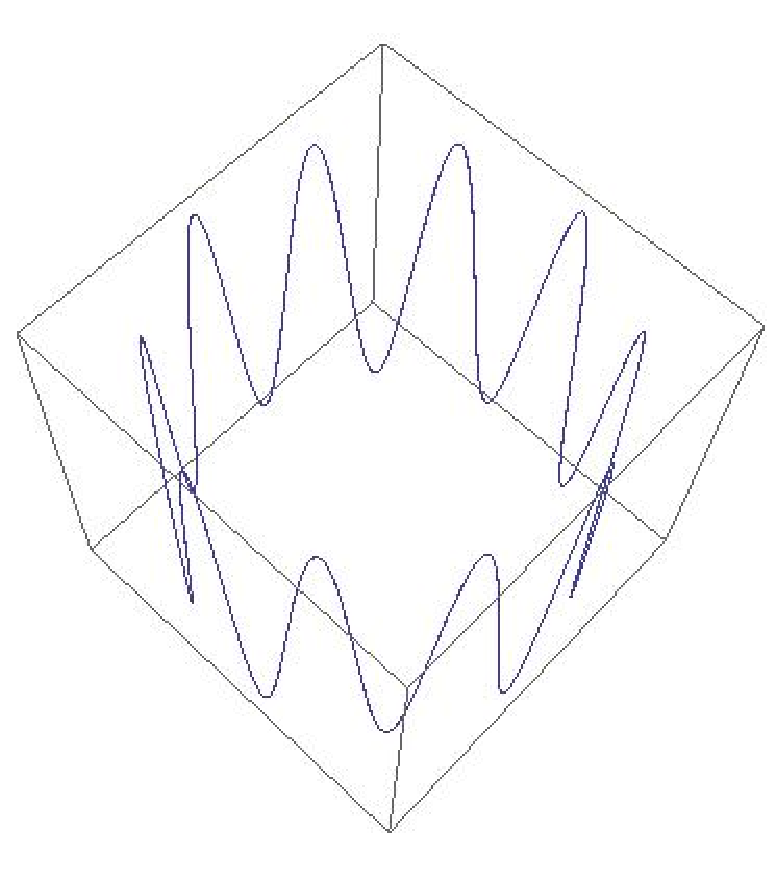
\psfig{file=jpegs/chapter-optical_lattice/fig1.eps,height=3.0in, width=5.0in}
 \caption{Representative diagram of a 'ringed lattice' with period $N=10$.}
 \label{fig:latticering:chapter-oplattice}
 \end{figure}

The interaction matrix elements (see appendix~\ref{appendix-matelements}) go as $\simeq 1/N$, and we set $N$ to 2. In the absence of external drives or interaction, this system reduces to the 2-quantum pendulum $H_{0i}(\kappa)=p_i^2+\kappa \cos{x_i}$, whose eigenstates are the Mathieu functions, and the eigenvalues are the characteristic functions of the Mathieu equation~\cite{abramowitz:stegun}. This is evidenced by looking at the numerically diagonalized eigenvalues in the absence of drives in Fig~\ref{fig:energylevels:chapter-oplattice}. States with $n>0$ are even parity states and states with $n<0$ are odd-parity states, a symmetry that is preserved if we use Eqn~\ref{eq:freeptcl:chapter-oplattice} for diagonalization. Note that $E_n\rightarrow n^2$ as $\kappa \rightarrow 0$, and $E_n\rightarrow n^2$ for large $|n|$ (the 'continuum' limit far above the pendulum separatrix in the classical phase space~\cite{reichl-appendix}).
%Fig 2
\begin{figure} 
\ 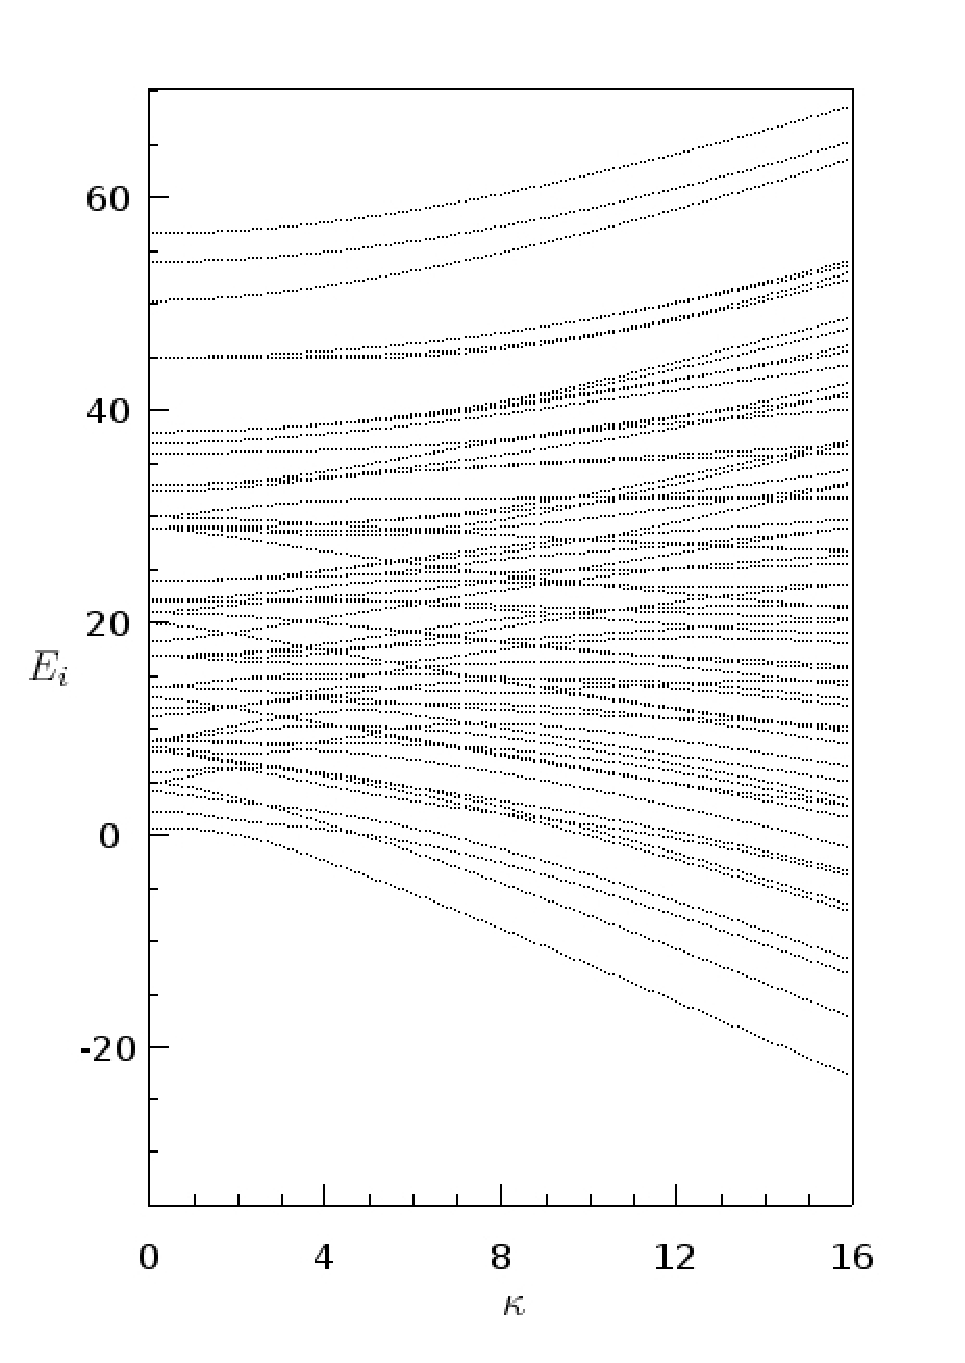
\psfig{file=jpegs/chapter-optical_lattice/fig2.eps,height=5.0in,width=3.0in}
\caption{Energy curves of the first $66$ lowest-energy states of both even and odd parities for the two-boson pendulum for the strongly interacting regime interaction amplitude $u_0=23.0$. Note the similarities with the characteristic functions for the Mathieu equation even for such a strong interaction.}
\label{fig:energylevels:chapter-oplattice}
\end{figure}

\section{\label{sec:3} Quantum Mechanics of the Interacting System}

We numerically diagonalize this Hamiltonian using the same nonadaptive finite element method used in section~\ref{chapter-dblwell:diaghamilt}, where the basis set is given by Eqn~\ref{eq:freeptcl:chapter-oplattice}. The 2-particle boson states of the box system are obtained by symmetrizing the 2-particle states to obtain a complete orthonormal basis of symmetrized 2-boson states:
%
\begin{equation}
{\langle}x_1,x_2\vert n_1,n_2{\rangle} ^{(s)}=\frac{1}{\sqrt{2(1+\delta_{n_1,n_2})}} 
[{\langle}x_1|n_1\rangle{\langle}x_2|n_2\rangle +{\langle}x_1|n_2\rangle{\langle}x_2|n_1\rangle ].
\label{eq:symm:chapter-oplattice}
\end{equation}
These states are then used to create a Hamiltonian matrix from Eqn.~\ref{eq:hamscale:chapter-oplattice}. The eigenvalues $E_i$ and eigenvectors $\vert E_i \rangle$ of the Hamiltonian matrix were determined numerically using the appropriate subroutine for diagonalizing real symmetric matrices in the GNU Scientific Library~\cite{galassi:gsl}. 


\subsection{The Strongly Interacting Regime}
As detailed in appendix~\ref{appendix-tof} for the double well problem, we wish to identify a 'strongly interacting regime' which will consist of a very strongly repulsive system and a moderate well depth. We define the 'strongly interacting factor' for this system, $\gamma$, as 
\begin{equation}
\gamma \equiv \frac{u_0}{E}.
\end{equation}
Here, $E$, the energy of the state, is a measure of the ability of the bosons to tunnel across from one well to another. When $\gamma \rightarrow \infty$, we reach the 'strongly interacting' regime where the system behaves line a Tonks gas, and the interaction completely dominates the system~\cite{tonks:gas}. The order parameter used to determine this is $p_i/{\delta l}$, where
\begin{equation}
p_i \equiv \delta l \int dx| \langle x,x | E_1 \rangle |^2.
\end{equation}
The order parameter $p_i$ is the total probability that the two particles lie arbitrarily close to each other within $\delta l$, and $i$ divides the $\gamma$-space into different regions of interest. Figure~\ref{fig:oplattice_tonksplot:chapter-oplattice} shows the plot of this  one dimensional probability density as a function of the strongly interacting factor. As expected, it vanishes for arbitrarily large values of $\gamma$, since the strong repulsions prevent two particles from being together. The transition to this regime is marked by a discontinuous change in the exponential decay of $p_i$ at $\gamma \sim 1.25$. The data points have been fitted to exponential decays,$\left( p_i/{\delta l} \right)=\left( p^0_i/{\delta l} \right) e^{-(\gamma/\gamma^0_i)}$ ,  by the use of numerical nonlinear least-squares algorithms. Here, $i$ denotes the region where the decay rate $\gamma^0$ appears to be fixed. We choose a value of $u_0=23.0$ for this particular value of $\kappa=4.9376435$ such that $\gamma=2.77465$, placing the system well in the region marked by $p_2$, and at a value of $p << p^0_1/e$.

%Fig 4
\begin{figure} 
\hspace*{-0.2in}
\ \psfig{file=jpegs/chapter-optical_lattice/fig4.eps,height=3.8in,width=5.7in}
\caption{Semi-logarithmic plot of the probability $\psi_i$ of two particles having the same position, as a function of the strongly interacting parameter $\gamma$ for a constant $\kappa=4.9376435$. The decay rate of $\psi$ changes sharply across $2$  regions, labeled by the index $i$. The data points (indicated by crosses and circles) have been fitted to exponential decay rates at each region (indicated by lines).The legend provides the numerically fitted values of the decay rates $\gamma^0_i$.}
\label{fig:oplattice_tonksplot:chapter-oplattice}
\end{figure}

\subsection{Energy Eigenstates}
Figures~\ref{fig:wavefunctions:chapter-oplattice}.a through~\ref{fig:wavefunctions:chapter-oplattice}.e are the probability distribution plots for the states $\langle x_1, x_2 | E_1 \rangle$, $\langle x_1, x_2 | E_3 \rangle$, $\langle x_1, x_2 | E_4 \rangle$,$\langle x_1, x_2 | E_5 \rangle$, and $\langle x_1, x_2 | E_{15} \rangle$ respectively at the value of $\kappa$ obtained in the section above. We chose these states because these transitions have the largest  amplitudes of $\cos{x}$, thus exhibiting significant Rabi oscillations. Note the presence of scarring in the wavefunctions of $|E_{14}\rangle$  and $|E_{18}\rangle$, where centroids seem to follow the classical trajectories for two bosons at that energy.

%Fig 5
\begin{figure} 
\ \psfig{file=jpegs/chapter-optical_lattice/fig5.eps,height=7.0in,width=2.0in}
\caption{Wavefunction plots for states 1, 3, 4, 5 , and 15}
\label{fig:wavefunctions:chapter-oplattice}
\end{figure}

\section{\label{sec:4} STIRAP Ladder, First Pulse $4 \leftrightarrow 15$, Second Pulse $1 \leftrightarrow 4$}
We now subject the system to a five resonance drive similar to the three-resonance drive done by Luter and Reichl~\cite{luter:reichl:3res} and Holder and Reichl~\cite{holder-reichl:avoidedcross} via STIRAP, using the five-resonance Hamiltonian defined by Eqn~\ref{eq:fiveres:chapter-oplattice}. In dimensionless form, this is 
\begin{eqnarray}
H=H_1(x_1,t)+H_2(x_2,t)+u_0 \delta(x_1-x_2) \\
H_i(x_i,t)=p_i^2 +\kappa \cos{x_i}+ \lambda_f \cos{x_i } \cos{ \omega_f t}+\lambda_s \cos{x_i} \cos{ \omega_s t}.
\end{eqnarray}
The drive for the five resonance Hamiltonian consists of two extra pairs of frequency-offset lasers, but drifting in opposite directions with speed $\omega_{f,s}$. The amplitudes of the lattices, $\lambda_{f,s}$, are slowly varying in time. Thus, 

\begin{equation}
H_i(t:t_{fix}) = \lambda^0  \cos{x_i} \left[ \lambda_f(t_{fix})\cos{\omega_f t} + \lambda_s(t_{fix}) \cos{\omega_s t}\right]
\end{equation}
for each particle. Here, 
\begin{equation}
 \lambda_{f,s}(t_{fix}) = e^{-(t_{fix}-t_{f,s})^2/4t^2_d},
 \label{eq:stirap:amp:chapter-oplattice}
\end{equation}
thus reproducing the time modulated radiation pulses characteristic of STIRAP as seen in sections~\ref{chapter-intro:section:stirap} and ~\ref{chapter-dblwell:section:stirap}. The driving frequencies $\omega_f=(E_{15}-E_4)$ and $\omega_s=(E_4-E_1)$. Thus, we are doing a ladder transition of the type $1\rightarrow 4 \rightarrow 15$ for a chosen value of $\kappa$ (see Fig~\ref{fig:stirap:chapter-oplattice}). 

If the two driving frequencies are rational factors ie $\omega_f/\omega_s = n_f/n_s$ for least common factor integers $n_{f,s}$, and the adiabatic time $t_{fix}$ varies slowly compared to the time period $T$ where
\begin{equation}
T=\pi \left(\frac{n_f}{\omega_f}+\frac{n_s}{\omega_s}\right),
\end{equation}
then the drive is time periodic and Floquet's theorem guarantees solutions of the type 
\begin{equation}
 |\psi_\alpha(t)\rangle=e^{-i\Omega_\alpha t}|\phi_\alpha(t)\rangle.
\end{equation}
Here, $|\phi_\alpha(t)\rangle$, the Floquet eigenstate(s) are $T$-periodic and $\Omega_\alpha$s are the Floquet eigenvalue(s), exactly as seen in  subsection~\ref{chapter-dblwell:section:qdynamics:subsec:floquet}. The value of $\kappa$ has been adjusted (see Fig~\ref{fig:stirap:chapter-oplattice}) to achieve commensurability of frequencies without requiring any detuning.

The matrix elements of Floquet evolution operator, $U_F(T)$, is given by
\begin{equation}
U_F(T) = \sum_{\alpha} e^{-i\Omega_{\alpha}T}|\phi_{\alpha}(0)\rangle\langle \phi_{\alpha}(0)|,
\end{equation}
%
and can be calculated numerically by integrating each column of the unit operator as the initial conditions by time $T$. This is done using an $8^{th}$ order Runge-Kutta Prince Dormand algorithm~\cite{rkutta:pd} from the GNU Scientific Library~\cite{galassi:gsl}, and the matrix diagonalized using a parallelized LAPACK library through the Scalable Library for Eigenvalue Problem Computations (Slepc)~\cite{slepc}. The eigenvalues, $e^{-i\Omega_{\alpha}T}$ can be used to obtain $\Omega_{\alpha}$ modulo one Floquet photon in the Brillouin zone as shown in subsection~\ref{chapter-dblwell:section:qdynamics:subsec:floquet}. A profile of the Floquet eigenvalues as a function of $t_{fix}$ provides a complete picture for the dynamics of the STIRAP process. As we have shown for the double well case in section~\ref{chapter-dblwell:section:stirap}, the Floquet eigencurves can be labeled by their dominant eigenstate or 'support state' (the energy eigenstates with which they are isomorphic at $t_{fix}=0$).
%Fig 3
\begin{figure} 
\ \psfig{file=jpegs/chapter-optical_lattice/fig3.eps,height=5.0in,width=5.0in}
\caption{Magnified view of energy curves shown in Fig~\ref{fig:energylevels:chapter-oplattice} with the value of $\kappa=7.287781$ chosen for the strongly interacting regime included. The levels being connected by STIRAP for this particular value of $\kappa$ are indicated. The value of $\kappa$ has been adjusted so that $\frac{\omega_f}{\omega_s}=\frac{3}{2}$}
\label{fig:stirap:chapter-oplattice}
\end{figure}

We chose to vary the STIRAP amplitudes as shown in Fig~\ref{fig:stirap_amps:chapter-oplattice}, with $\lambda_0=0.2$, $t_f=(1/3) t_{tot}$, $t_s=(2/3)t_{tot}$, and the pulse widths $t_d=(1/14)t_{tot}$. Here $t_{tot}$ defines the total time scale for both pulses, and $t_{fix}$ is expressed in units of $t_{tot}$ unless otherwise stated, the $t_{tot}$ dependence on $\Omega_\alpha$ being negligible~\cite{na-reichl:pbox}~\cite{na-reichl:mol-rot}~\cite{na-reichl:isomer}. Figure~\ref{fig:floquet_quasi_0.2:chapter-oplattice} shows the Floquet eigenvalues of the relevant Floquet eigenstates as the system evolves in adiabatic time. The relevant eigenstates are the ones isomorphic to the states connected by the STIRAP pulses viz. $|E_1\rangle$, $|E_4\rangle$, and $|E_{15}\rangle$. We notice that the eigenvalues are degenerate at $t_{fix}=0$ and $t_{fix}=t_{tot}$ as expected. We also note a higher order resonance that brings $|E_{18}\rangle$ into the degenerate subspace. The Floquet states and corresponding quasienergies are labeled alphabetically as follows:
\begin{enumerate}
 \item
The eigenphase whose corresponding Floquet eigenstate is supported by the undriven  state $|E_{18}{\rangle}$  at $t_{fix}=0$ is labeled as $\Omega_A$ and the Floquet eigenstate as $|\phi_A\rangle$.
\item
The eigenphase whose corresponding Floquet eigenstate is supported by the undriven state $\frac{1}{\sqrt{2}}\left[|E_4\rangle - |E_{15}\rangle \right]$ at $t_{fix}=0$ is labeled as $\Omega_B$ and the Floquet eigenstate as $|\phi_B\rangle$.
\item
The eigenphase whose corresponding Floquet eigenstate is supported by the undriven state $\frac{1}{\sqrt{2}}\left[|E_4\rangle + |E_{15}\rangle \right]$ at $t_{fix}=0$  is labeled as $\Omega_C$ and the Floquet eigenstate as $|\phi_C\rangle$.
\item 
The eigenphase whose corresponding Floquet eigenstate is supported by the undriven ground state $|E_1{\rangle}$  at $t_{fix}=0$ is labeled as $\Omega_D$ and the Floquet eigenstate as $|\phi_D\rangle$.
\end{enumerate}
%Fig 6
\begin{figure} 
\ 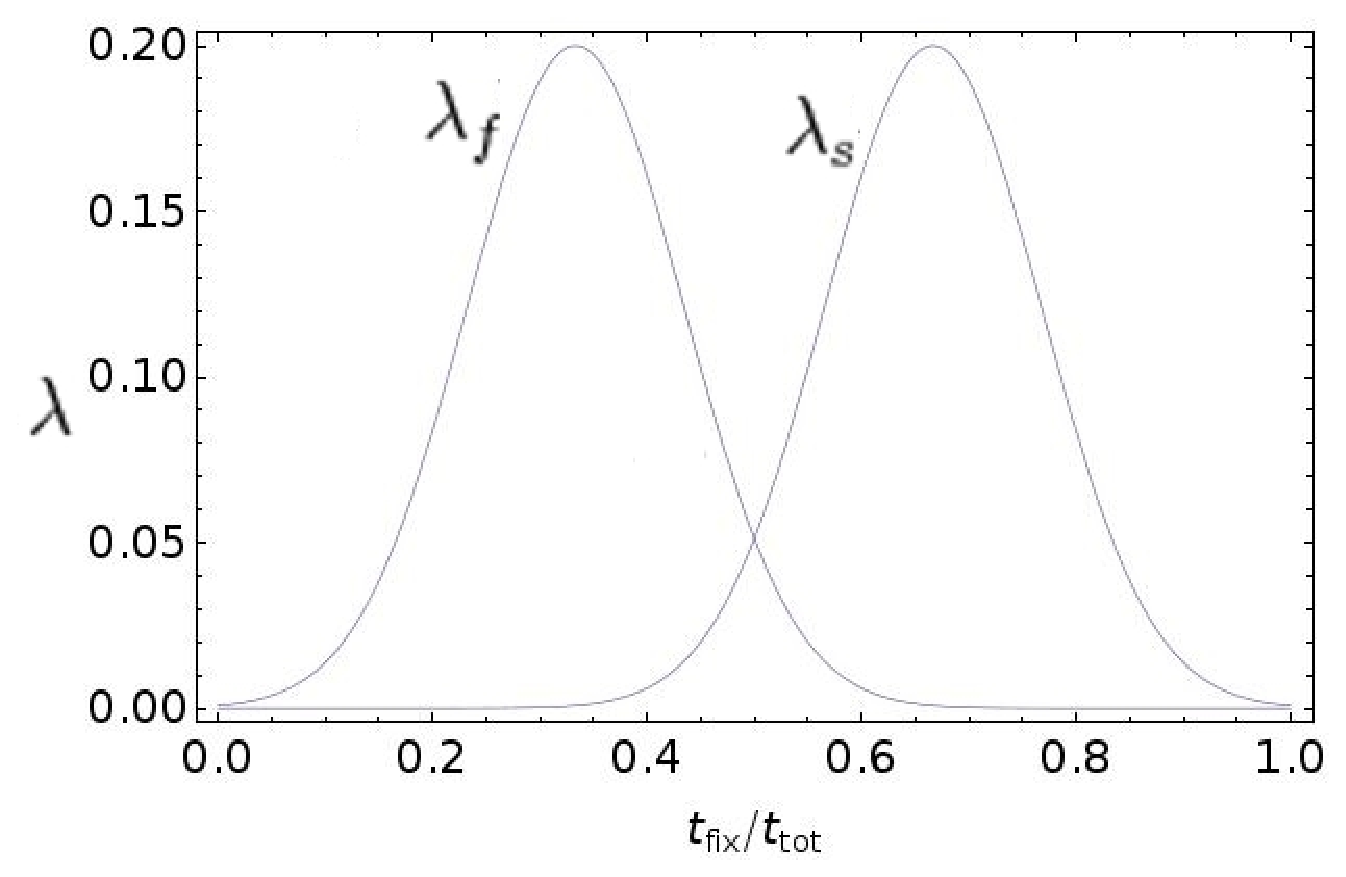
\psfig{file=jpegs/chapter-optical_lattice/fig6.eps,height=3.0in,width=5.0in}
\caption{The amplitudes $\lambda_{f,s}$ of the STIRAP pulses as a function of time with $\lambda_0=0.2$ (see Eqn~\ref{eq:stirap:amp:chapter-oplattice}). The first pulse (in time)  connects the intermediate state to the final state of the STIRAP process. All units are dimensionless. The second pulse (in time)  connects the initial state and the intermediate state. The total time $t_{tot}$ is chosen arbitrarily, but the centroids of the pulses are kept at $\frac{t_f}{t_{tot}}=\frac{1}{3}$,$\frac{t_s}{t_{tot}}=\frac{2}{3}$,$\frac{t_d}{t_{tot}}=\frac{1}{14}$,where $t_{f,s}$ are the centroids of the first and second pulses respectively, and $t_d$ is the width of the pulses.}
\label{fig:stirap_amps:chapter-oplattice}
\end{figure}

Thus, the system, if evolving adiabatically, stays in $\Omega_D$ at all times, and avoids all avoided crossings that it encounters during STIRAP. We notice signs of traditional $3$-level avoided crossing for the system at $t_{fix}\simeq 0.5$ $t_{tot}$ in Fig~\ref{fig:floquet_quasi_0.2:chapter-oplattice}. However, we notice additional avoided crossings in $\Omega_D$ that will affect the transitions in the system. First, $\Omega_D$ appears to undergo an avoided crossing with $\Omega_A$ at $t_{fix}\simeq 0.45$ $t_{tot}$, exchanging characteristics of $|\phi_D\rangle$ in the process. The traditional 3-level STIRAP transition occurs after this event. Before the dynamics is complete, however, another avoided crossing occurs between $\Omega_D$ and $\Omega_A$, also causing the character of $|\phi_D\rangle$ in the process. Thus, the final outcome of a stimulated Raman adiabatic passage will be very different from traditional STIRAP if the crossings are navigated by adiabatic passage. The dependence of $|\phi_A\rangle$ through $|\phi_D\rangle$ on the unperturbed energy eigenstates is shown in Fig~\ref{fig:floquet_states_0.2:chapter-oplattice}. The influence of the avoided crossings is clearly seen. The final outcome is a linear superposition of the type $\frac{1}{\sqrt{2}}(|E_1\rangle \pm |E_4\rangle)$. These avoided crossings are manifestations of classical chaos in the quantum dynamics similar to the ones seen for the double well system in chapter~\ref{chapter-dblwell}.
  
The dynamics can be analyzed in more detail by using the Landau-Zener formula to calculate the probability of a transition at an avoided crossing. The probability $P_{\alpha\beta}$ for an avoided crossing between two Floquet eigenphases $\Omega_{\alpha}$ and $\Omega_{\beta}$ to be crossed  is given by (see Eqn~\ref{eq:lzformula:chapter-intro})
\begin{equation}
P_{\alpha \beta}=\exp\left[-\frac{\pi ({\delta \Omega_{\alpha \beta}})^2}{2\Gamma_{\alpha \beta}}\right],
\label{eq:landauzener:chapter-oplattice}
\end{equation}
%
%
where $\delta\Omega_{\alpha\beta}$ is the (minimum) spacing  between $\Omega_\alpha$ and $\Omega_\beta$ at the avoided crossing and $\Gamma_{\alpha\beta}$   is the magnitude of the  rate of change (slope) of the Floquet eigenphases in the immediate neighborhood of the avoided crossing. Thus,
%
\begin{equation}
\Gamma_{\alpha\beta} = {\biggl|} \frac{d\Omega_\alpha}{dt} - \frac{d\Omega_\beta}{dt}{\biggr|},
\label{eq:gamma:chapter-oplattice}
\end{equation}
%
where  $\frac{d\Omega_\alpha}{dt}$ is the slope of the  eigenphase curve $\Omega_\alpha$ in the neighborhood of the avoided crossing. We follow the derivation of the Landau-Zener formula for the double well system in previous chapters to get 
\begin{equation}
P_{\alpha \beta}=\exp\left[-t_{tot}{\gamma}_{\alpha,\beta} \right].
\label{eq:lanzen:chapter-oplattice}
\end{equation}
%
where ${\gamma}_{\alpha,\beta}=\frac{\pi ({\delta \Omega_{\alpha \beta}})^2}{2{\bar \Gamma}_{\alpha \beta}}$. 

In order for a crossing to be avoided instead of crossed, $P_{\alpha\beta}\approx 0$, and the actual time scale of the STIRAP must be adjusted accordingly. Thus, the transfer probability $P_{\alpha \beta}$ will be very small if $t_{tot}>1/{\gamma}_{\alpha,\beta}$. 
Figures~\ref{fig:floquet_states_0.2:mag:chapter-oplattice}.a and~\ref{fig:floquet_states_0.2:mag:chapter-oplattice}.b show magnified plots of the eigenphases at the two avoided crossings described above. For the first $AD$ avoided crossing shown in Fig~\ref{fig:floquet_states_0.2:mag:chapter-oplattice}.a, we estimate the gap $\delta \Omega_{AD}$ to be $3.67 \times 10^{-4}$, and $\Gamma_{AD}$ to be $0.0155$, rendering $\frac{2\gamma_{AD}}{\pi}$ to be $8.6803 \times 10^{-7}$. Thus $t_{tot}>7.334 \times 10^{4}$. Similarly, for the second $BD$ avoided crossing (Fig~\ref{fig:floquet_states_0.2:mag:chapter-oplattice}.b), $\delta \Omega_{BD}\simeq 1.984 \times 10^{-3}$, and  $\Gamma_{BD}\simeq 0.135$, concluding that $t_{tot}>2.184 \times 10^4$. For $^{85}Rb$, we noted in section~\ref{chapter-intro:section:lightatom:subsec:2lvl} that the $D_2$ transition line is is about $780$ $nm$ (see Fig~\ref{fig:rblevels}). The recoil frequency, $ \omega_r$ is thus about $24$ $KHz$. The characteristic time scale here is $1/(4\omega_r)$, or $1.03 \times 10^{-5}$ seconds. We can plug this value to the minimum value(s) of $t_{tot}$ to get the actual time. Thus, for the $^{85}Rb$ atom, we get $t_{tot}>0.756$ $sec$ for the $AD$ crossing and $t_{tot}>0.225$ $sec$ for the $BD$ crossing. Thus, the $BD$ crossing is automatically avoided if the $AD$ crossing is avoided, making the most rapid required time scale for both chaos assisted adiabatic passages to be $0.756$ seconds. If the time scale for the stirap is faster than $0.225$ seconds, then neither crossing is avoided and traditional 3-level STIRAP will be seen.
%fig 7
\begin{figure} 
\vspace*{-0.1in}
\ 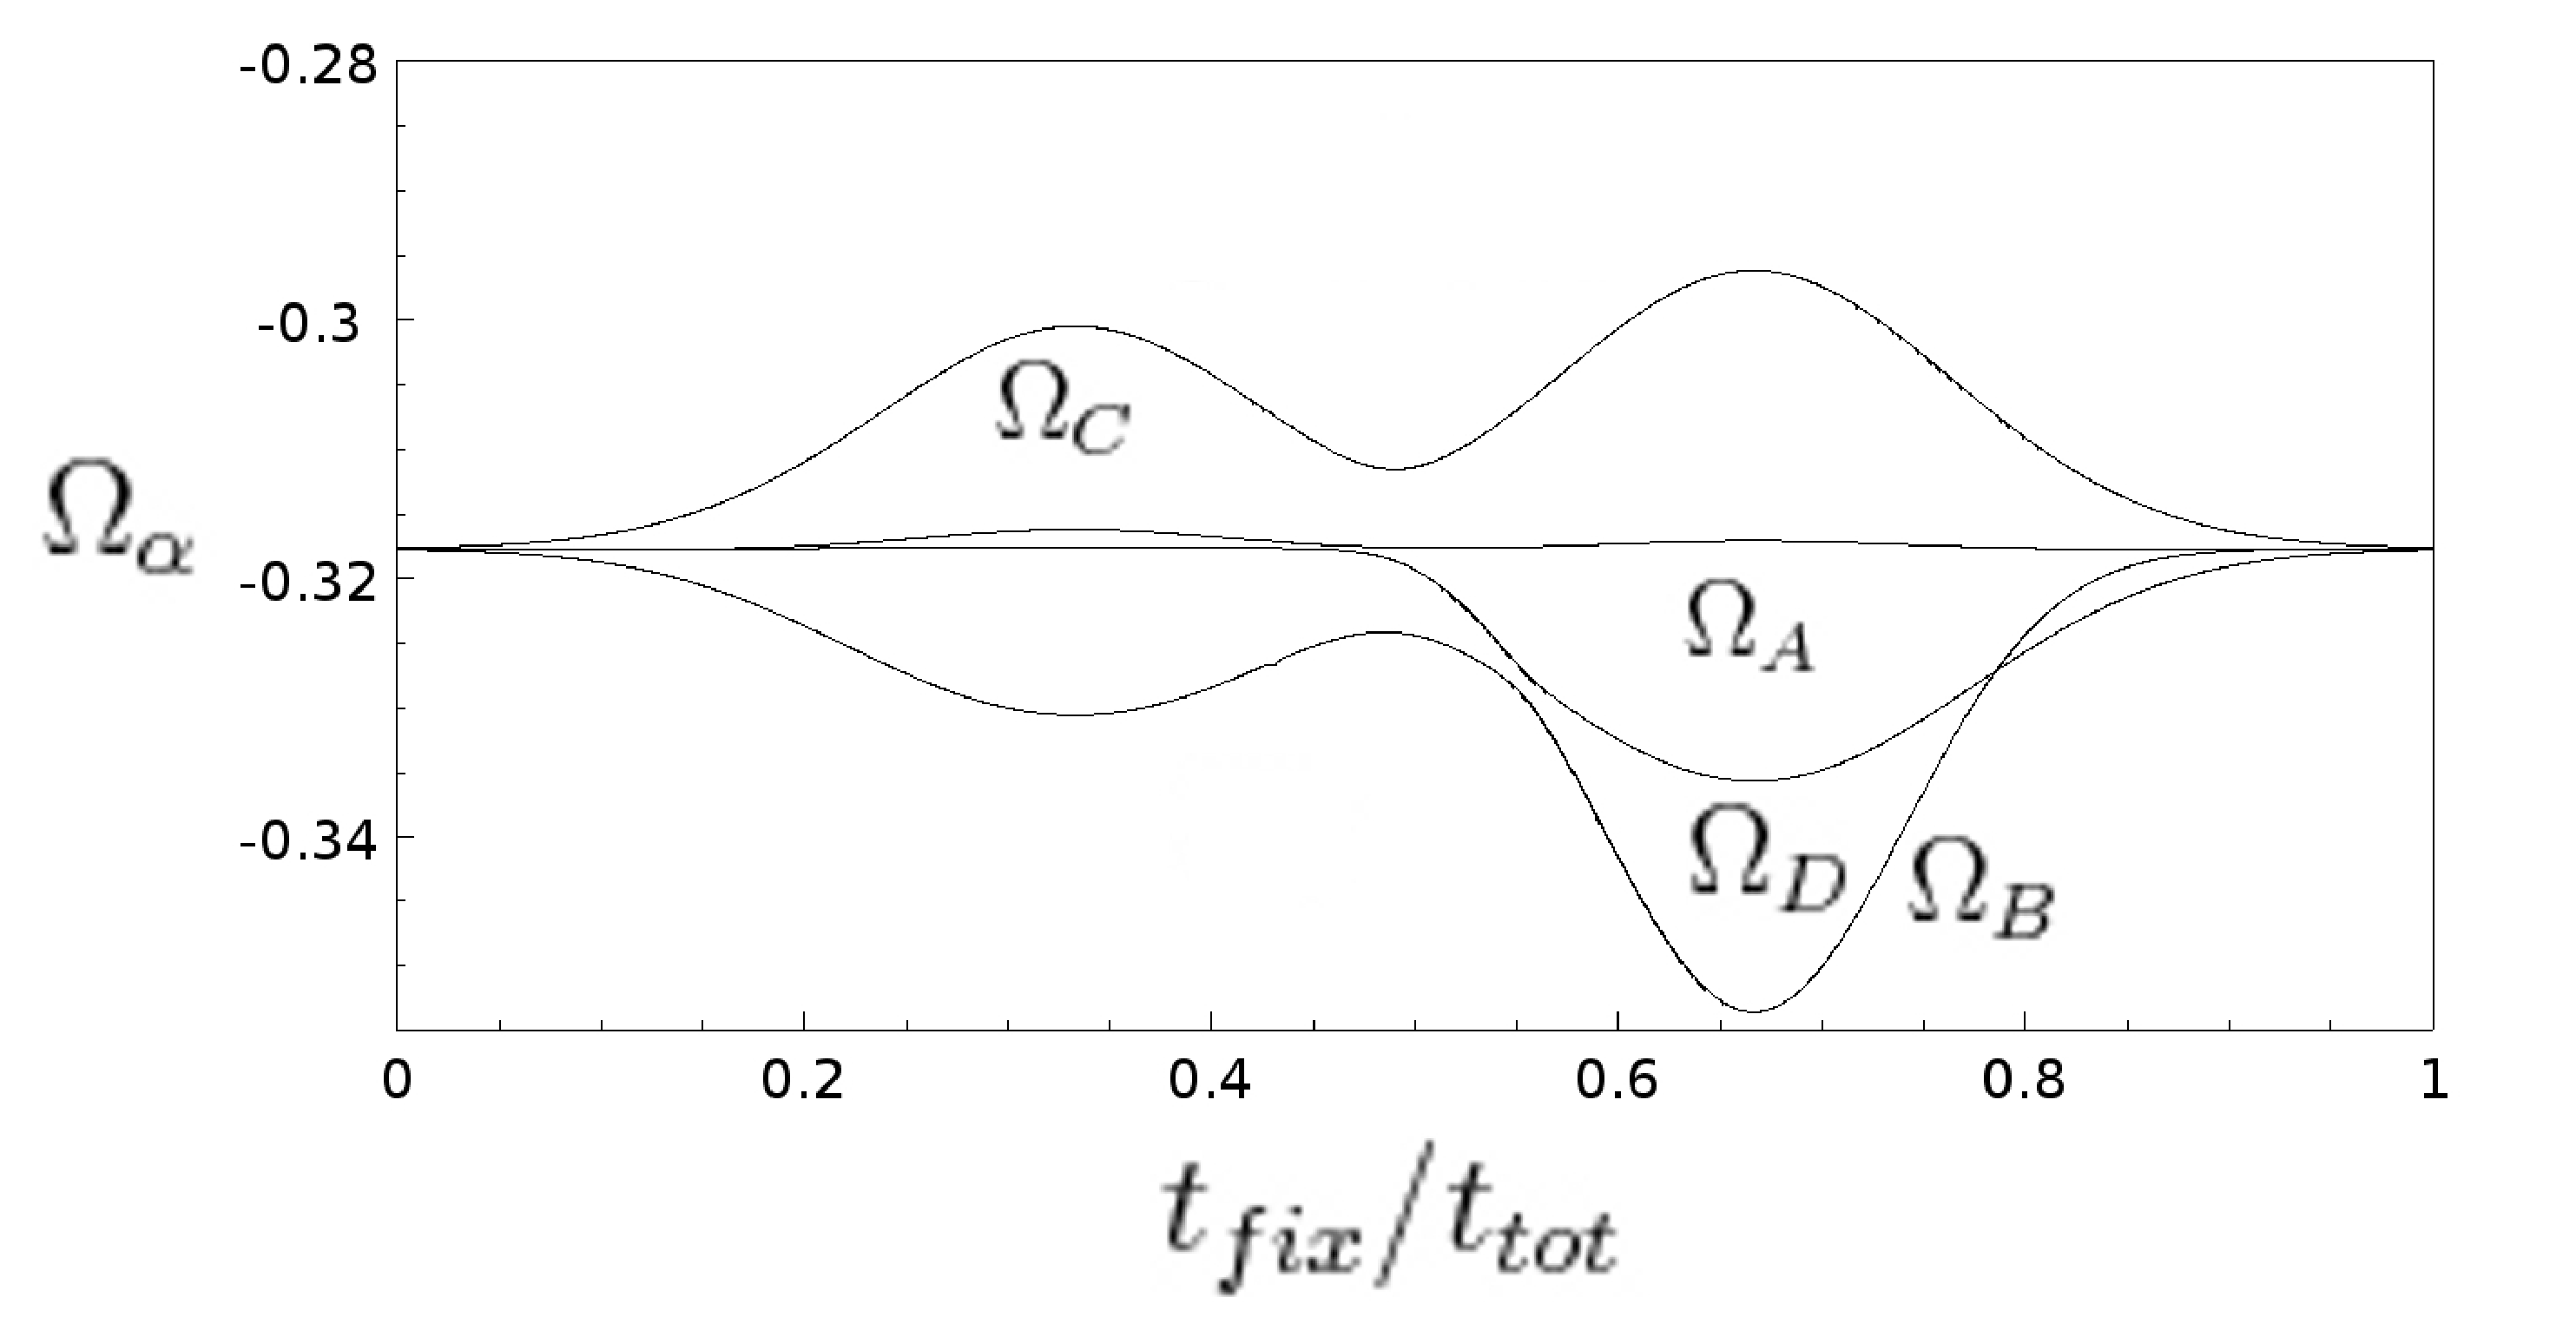
\psfig{file=jpegs/chapter-optical_lattice/fig7.eps,height=3.5in,width=4.6in}
\caption{Floquet quasienergies $\Omega_{\alpha}$ as a function of adiabatic time $t_{fix}/t_{tot}$ for $\lambda^0=0.2$. the labels $\Omega_{A-D}$ denote the floquet quasienergy curves corresponding to the Floquet eigenstates $|\phi_{A-D}\rangle$ respectively. The Brillouin zone is $\left[-\frac{\omega}{2}, \frac{\omega}{2}\right]$}
\label{fig:floquet_quasi_0.2:chapter-oplattice}
\end{figure}
%Fig 8
\begin{figure} 
\ 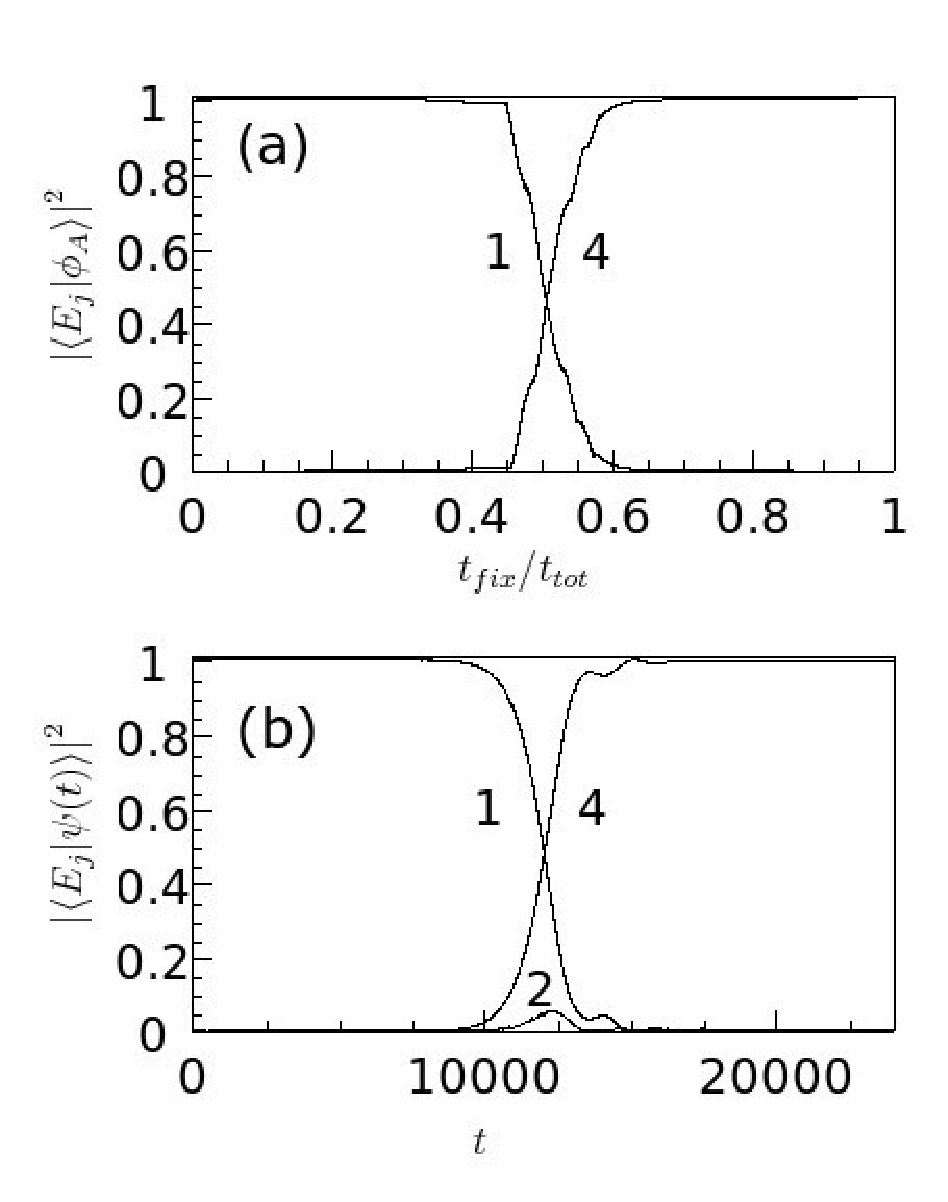
\psfig{file=jpegs/chapter-optical_lattice/fig8.eps,height=6.0in,width=3.0in}
\caption{Plot of the Floquet eigenfunctions $\langle E_i|\phi_{A-D}\rangle$ in the undriven Hamiltonian representation. The components of the Floquet states in each energy level are numbered. Note the influence of the avoided crossings in $|\phi_D\rangle$.}
\label{fig:floquet_states_0.2:chapter-oplattice}
\end{figure}
%Fig 9
\begin{figure} 
\ 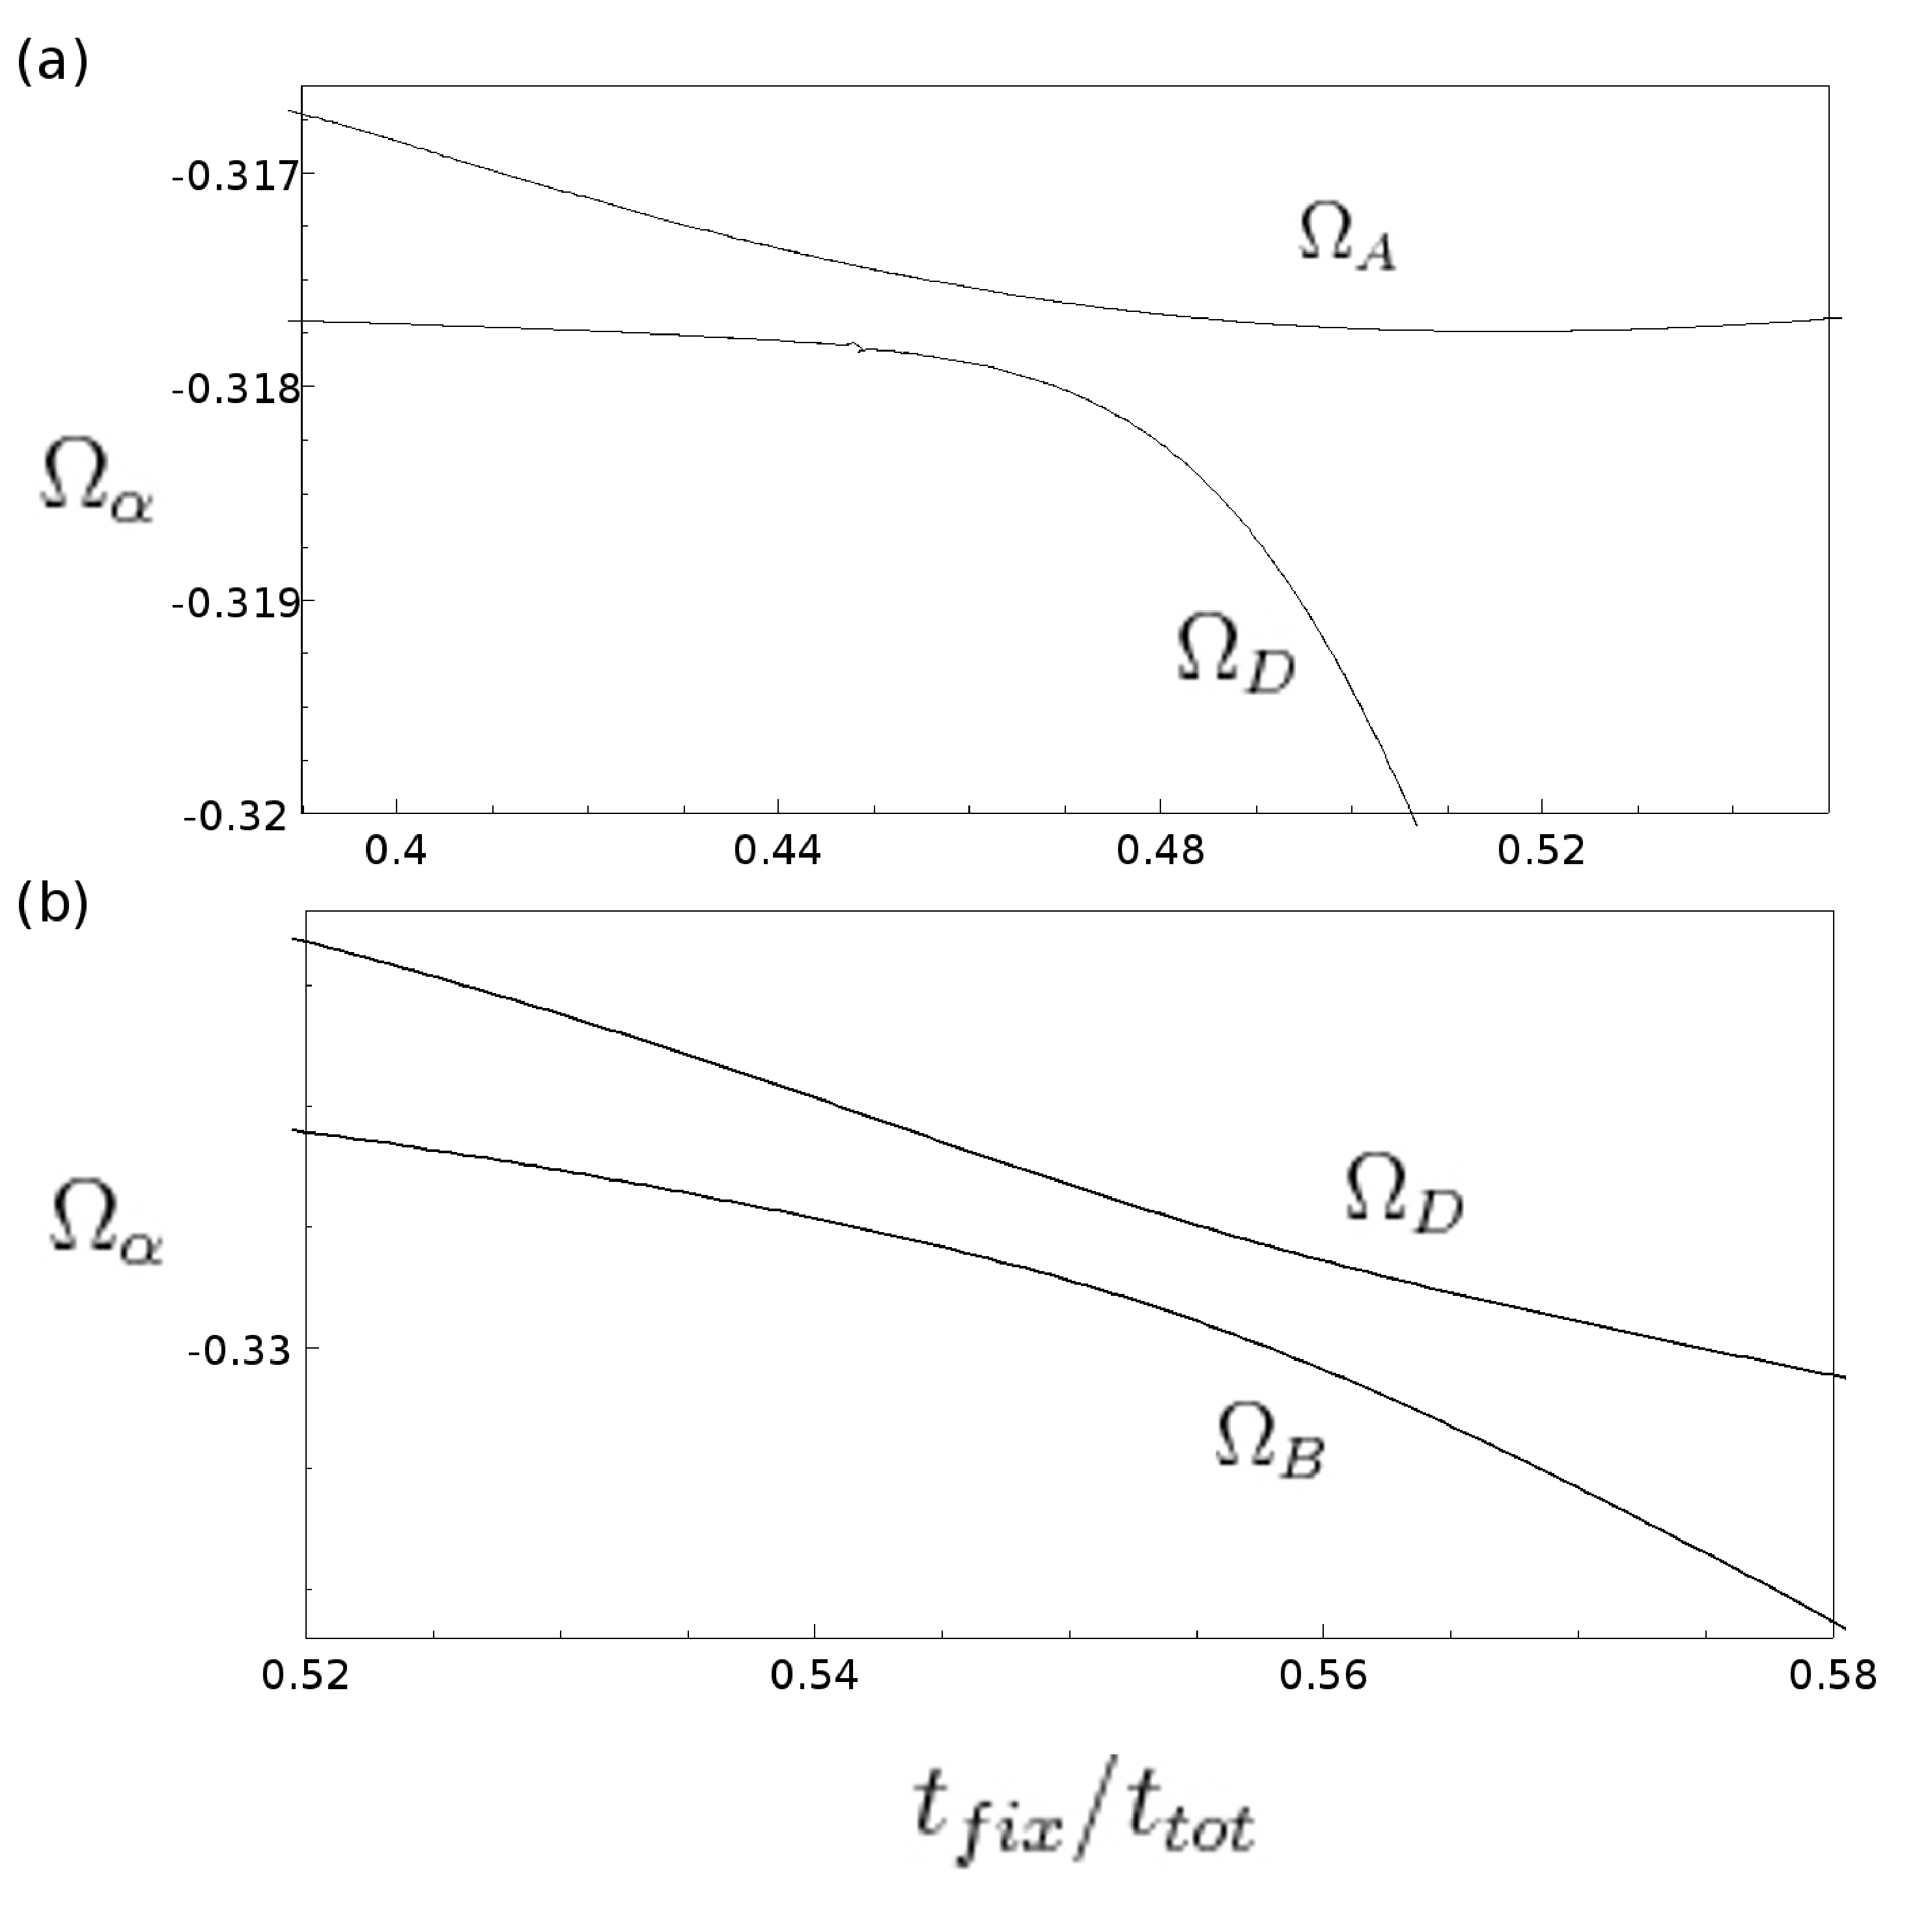
\psfig{file=jpegs/chapter-optical_lattice/fig9.eps,height=6.5in,width=4.5in}
\caption{Magnified views of the $AD$ and $BD$ avoided crossings from the Floquet eigenphase plots in Fig~\ref{fig:floquet_quasi_0.2:chapter-oplattice}. Figure (a) shows the $AD$ crossing and Fig (b) shows the $BD$ crossing. As in Fig~\ref{fig:floquet_quasi_0.2:chapter-oplattice}, the quasienergies $\Omega_\alpha$ are plotted as a function of $t_{fix}/t_{tot}$, where $t_{tot}$ is the total time for the STIRAP pulses.}
\label{fig:floquet_states_0.2:mag:chapter-oplattice}
\end{figure}

\chapter{Conclusion}
\index{Conclusion@\emph{Conclusion}}%
\label{chapter-conclusion}
We have analyzed the dynamics of interacting two-boson systems for ultracold alkali metal atoms in electromagnetic traps. We have modeled double well potentials for those traps using magnetic confinement in atom chips as well as far-off resonance traps in optical lattices. The reduced atom Hamiltonian, when subjected to time-modulated sinusoidal drives, will undergo excitations to higher states, the transition to which can be coherently controlled by stimulated Raman adiabatic passage (STIRAP).

We have observed some unusual behavior in the classical and quantum dynamics of two bosons in a double well, where the interaction between them is weakly repulsive (the 'single particle regime'). Chaos in the separatrix region of the classical version of the coupled system corresponds with regions of high probability in the quantum Poincare map. However, a noticeable tunneling has been observed from the separatrix into the individual wells. We have also demonstrated the feasibility of a controlled excitation of the system into a higher energy state using STIRAP using external radiation pulses that cause dipole excitations. Avoided crossings in the Floquet eigenphases arise due to level repulsion caused by a loss of symmetry as they evolve adiabatically with time, and are connected with the dynamics of the underlying classical system. The classical dynamics of the system in those regions of the parameter space are nonintegrable, and the presence of multiple nonlinear resonances cause transitions to chaos from KAM tori~\cite{reichl}. A system undergoing a chaos-assisted adiabatic passage by avoiding these crossings will manifest quantum effects due to the classical chaos~\cite{reichl}~\cite{latka:avoidedcrossings:chaos}. Thus, the driving fields induce nonlinear resonances and chaos in localized regions of the phase space that affect the structure of the Floquet eigensystem and influence the STIRAP dynamics accordingly~\cite{na-reichl:pbox}. We have looked at the controlled dynamics of STIRAP from the ground state of such a system to the third excited state for small and large STIRAP pulse amplitudes. 

For sufficiently large amplitudes, the effects of the underlying classical dynamics start to manifest themselves through small avoided crossings between the involved Floquet eigenphases.  The first avoided crossing causes a change in character between the ground state and a linear combination of the other two states states that are connected by the STIRAP pulses. However, the second avoided crossings (of the same type as the first one) between the same eigenphases causes the character change to reverse. Thus, these avoided crossings cause a temporary loss in coherence of the wavefunction as it evolves from the ground state, after which the system proceeds to complete the dynamics as expected for an ordinary three level STIRAP, completely populating the final state of the system. The time scale (of the STIRAP pulses) for such avoided crossings to be avoided (so that the chaos assisted adiabatic passage that causes the character changes may occur) was computed from the numerical data using the Landau-Zener formula. 

The required pulse times for such a system turned out to be very slow at $1.62 \times 10^5$ units of $T_u$, where $T_u=\frac{2mL^2_u} {\hbar}$ for atoms of mass $m$ (chosen to be that of $^{85}Rb$ alkali metal atoms) and a quartic double well system with well minima at length $L_u$. This was confirmed by numerical simulations of the exact quantum dynamics, where the population transfers were seen for small pulse times and the effects of the avoided crossings seen for larger pulse times. If we use double wells of $L_u\simeq 50$ $nm$, then $T_u=6.68118$ $\mu s$, making the time scale for the avoided crossings to be $1.08235$ seconds. For optical systems, the double wells would be at least one order of magnitude larger, making the time scale two orders larger (nearly $2$ minutes). We also looked at STIRAP in a slightly adjusted well depth for which the chaos produced by additional resonances produce avoided crossings that can cause coherent population transfer to a higher state (in our case, the sixth excited state). This defect was verified for the exact time evolution of the system as well. The physical time scale for this crossing to be avoided was determined to be $1.2 \times 10^3$ units of $T_u$, which, for  $L_u\simeq 50$ $nm$, translates to $8.01742$ $ms$. For optical lattice systems, these time scales would increase by two orders of magnitude.  Thus, we demonstrated radiation pulses can be used to exert coherent control of the coupled boson system through chaos assisted adiabatic passages, just as has been recorded for systems with lower degrees of freedom.

We then proceeded to look at a similar dynamical system in an optical lattice generated by two counter-propagating lasers, except with stronger repulsive interaction. Time modulations in the frequencies of these lasers produce non-dipole excitations that can be controlled in a manner similar to our earlier system. The STIRAP pulses were tuned to connect very high energy states (the final state being the fourteenth excited state). The presence of an additional resonance with the seventeenth excited state, along with avoided crossings between the other states connected by STIRAP, cause the outcome of STIRAP to differ from the traditional three level case in a way similar to our previous system. We noticed two avoided crossings, one between the ground state and the fourteenth excited state that causes them to switch character with a time scale of $7.334 \times 10^4$ units of time (The characteristic time scale here is $1/(4\omega_r)$, where $\omega_r$ is the recoil frequency of the optical lattice and can be calculated from the wavelength, which is slightly detuned away from the $D_2$ transition line of $^{85}Rb$ as $1.03 \times 10^{-5}$ seconds). Thus, the physical time scale for this crossing is $0.756$ seconds. After this crossing is avoided, another crossing was seen between the ground state (now with character switched) and one of the states connected by STIRAP (a linear combination of the third and fourteenth excited states). The time scale for this crossing to be avoided was calculated for the $D_2$ transition line to be $0.225$ seconds. 

Thus, both crossings are avoided if the first one is avoided, resulting in a complete loss of coherence in the final outcome. STIRAP pulses with faster time scales will cause these crossings to be crossed with no change in eigenstate character. Thus, traditional three-level stirap will be seen, resulting in a  coherent population transfer to the fourteenth excited state. This effect of the underlying classical chaos will prove useful in understanding the coherent dynamics of excitations in systems of optical lattices that have been replicated in the laboratory, and is vital to the outcome of experiments involving coherent acceleration of bosons in optical lattices.
%%%%%%%%%%%%%%%%%%%%%%%%%%%%%%%%%%%%%%%%%%%%%%%%%%%%%%%%%%%%%%%%%%%%%%
% Appendix/Appendices                                                %
%%%%%%%%%%%%%%%%%%%%%%%%%%%%%%%%%%%%%%%%%%%%%%%%%%%%%%%%%%%%%%%%%%%%%%
%
% If you have only one appendix, use the command \appendix instead
% of \appendices.
%
\appendices
\index{Appendices@\emph{Appendices}}%

\chapter{Matrix Elements for two Bosons}
\index{Appendix!Matrix Elements for two Bosons @\emph{Matrix Elements for two Bosons}}%
\label{appendix-matelements}
\section{Introduction}
The Hamiltonians in the text of this dissertation are diagonalized numerically by a nonadaptive finite element method using the matrix elements in a suitable known basis.A tower of states for the 2-particle system are built up by index using unique combinations of single particle states up to the truncation value $N$. Thus, the tower consists of the combinations of the type $n=\left[i,j\right]$, where $n$ is the index for the two-particle state and $i$, $j$ are the corresponding single particle eigenstate indices. The decomposition of the tower of states is detailed on table~\ref{tabA:appendix}.

\begin{table}
\begin{center}
\begin{tabular}{|c|c|c|c|c|c|c|c|c|}
\hline
$n$ & $\left[i,j\right]$&	$n$&$\left[i,j\right]$&	$n$&$\left[i,j\right]$&	$\hdots$&	$n$&$\left[i,j\right]$\\
\hline
1&$\left[1,1\right]$&	&	&	&	&	&	&	\\
2&$\left[1,2\right]$&$N+1$&$\left[2,2\right]$&	&	&	&	&	\\
3&$\left[1,3\right]$&$N+2$&$\left[2,3\right]$&$2N+1$&$\left[3,3\right]$&$\hdots$&	&	\\
$\vdots$&$\vdots$&$\vdots$&$\vdots$& $\vdots$& $\vdots$&$\hdots$&	&	\\
$N$&$\left[1,N\right]$&$2N-1$&$\left[2,N\right]$&$3N-2$&$\left[3,N\right]$&$\hdots$& $N^2-N+1$& $\left[N,N\right]$\\
\hline
\end{tabular}
\caption{Tower of states $n=\left[i,j\right]$ constructed for the diagonalization of the two-boson system. Here, $n$ is the index for the two-particle state and $i$, $j$ are the corresponding single particle eigenstate indices.}
\label{tabA:appendix}
\end{center}
\end{table}
The matrix elements can now be evaluated after each member in the tower of states is assigned to a two-particle state decomposition as follows.
\begin{equation}
{\langle}x_1,x_2\vert n_1,n_2{\rangle} ^{(s)}=\frac{1}{\sqrt{2(1+\delta_{n_1,n_2})}} 
[{\langle}x_1|n_1\rangle{\langle}x_2|n_2\rangle +{\langle}x_1|n_2\rangle{\langle}x_2|n_1\rangle ],
\label{eq:symm:appendix}
\end{equation}

Thus, the matrix element of an operator $A=a_1+a_2$, where $a_i$ is the corresponding single particle operator for the $i^{th}$ particle,  can be decomposed into single particle matrix elements as follows
\begin{multline}
\langle n | A| m \rangle =\frac{1}{\sqrt{2(1+\delta_{n_1,n_2})}} \frac{1}{\sqrt{2(1+\delta_{m_1,m_2})}}\\
  \left[ \langle n_1|a|m_1\rangle \delta_{n_2 m_2} +  \langle n_1|a|m_2\rangle \delta_{n_2 m_1}+ 
  \langle n_2|a|m_1\rangle \delta_{n_1 m_2}+\langle n_2|a|m_2\rangle \delta_{n_1 m_1} \right]
\end{multline}
Here, the states $|m\rangle$ and $|n\rangle$ for the two-particle system are broken up into $|m_1,m_2\rangle$ and $|n_1,n_2\rangle$ respectively, where $m=\left[m_1,m_2\right]$ and $n=\left[ n_1,n_2\right]$ as shown in table~\ref{tabA:appendix}.
\section{Double Well}
The Hamiltonian for two bosons in a quartic double well adiabatically driven by laser pulses  is given by
\begin{eqnarray}
H(t;t_{fix})=H+\left[\epsilon_f(t_{fix})\sin(\omega_ft)+\epsilon_s(t_{fix})\sin(\omega_st)\right](x_1+x_2),\\
H =p^2_1+p^2_2+V_0 (-2 x_1^2+ x_1^4) +V_0 (-2 x_2^2+ x_2^4)+U_0 \delta(x_1-x_2).
\label{eq:fullham:appendix}
\end{eqnarray}
In the case of the double well, we have chosen the eigenbasis of two bosons on a box of size $L$ (in accordance with~\cite{na-reichl:pbox}). The box size $L$ is optimized for the best possible convergence of the ground state energy. Therefore, the single particle basis is
\begin{equation}
\langle x|n,x\rangle=\frac{1}{\sqrt{L}} \sin{\biggl[}{\frac{n\pi}{2}(\frac{x}{L}-1){\biggr]}},
\label{eq:pboxfn:appendix}
\end{equation}
%
within the box (and vanishing outside). Here, $n=1,2,...N$. 

Thus, the matrix elements of the single particle operators $p^2$, $x$, $x^2$ and $x^4$ for a particle in a box need to be evaluated. Since the particle in a box has a Hamiltonian of $p^2$ within the box (and infinity outside), the matrix elements are
\begin{equation}
 \langle m_i |p^2| n_i \rangle=\frac{n^2_i\pi ^2}{4L^2} \delta_{m_in_i}.
\label{eq:psqmat:appendix}
\end{equation}
The matrix elements of $x$ for a particle in a box are given by
\begin{equation}
 \langle m_i |x| n_i \rangle = \left\{
\begin{array}{lll}
\frac{16m_in_i}{\pi ^2\left(m_i^2-n_i^2\right)^2}L & m_i+n_i \mbox{ is odd }, \\
0 & \mbox{otherwise.}
\end{array}
\right.
\end{equation}
Similarly, the matrix elements of $x^2$ for a particle in a box are
\begin{equation}
\langle m_i |x^2| n_i \rangle = \left\{
\begin{array}{lll}
\frac{32m_in_i}{\pi ^2\left(m_i^2-n_i^2\right)^2}L^2 & m_i+n_i  \mbox{ is even, and } m_i \neq n_i,  \\
\left(\frac{1}{3}-\frac{2}{n_i^2\pi ^2}\right)L^2 & m_i=n_i, \\
0 & \mbox{otherwise.}
\end{array}
\right.
\end{equation}
The matrix elements of $x^4$ are likewise given by
\begin{equation}
 \langle m_i |x^4| n_i \rangle = \left\{
 \begin{array}{lll}
\frac{64m_in_i}{\pi^4}   \left[ \frac{\pi^2}{(m_i^2 - n_i^2)^2} - \frac{
   48(m_i^2 + n_i^2)}{(m_i^2 - n_i^2)^4}\right] L^4 & m_i+n_i  \mbox{ is even, and } m_i \neq n_i, \\
\left(\frac{1}{5}-\frac{4}{n_i^2\pi ^2}+\frac{24}{n_i^4\pi ^4}\right)L^4 & m_i=n_i,\\
0 & \mbox{otherwise.}
\end{array}
\right.
\end{equation}
The matrix elements of the two-particle interaction operator are shown below.
\begin{equation}
\frac{1}{2} \langle m | \delta(x_1-x_2) | n \rangle =\left\{
\begin{array}{lll}
-\frac{1}{4L} & \left\{ \begin{array}{lll}
 & n_1-n_2=m_1+m_2 \mbox{ , and } n_1\neq n_2,\\
 & n_1+n_2=m_2-m_1 \mbox{ , and } n_1\neq -n_2,\\
 & n_1+n_2=m_1-m_2 \mbox{ , and } n_1\neq -n_2,\\
 & n_1-n_2=-m_1-m_2 \mbox{ , and } n_1\neq n_2\\
 \end{array}\right\}, \\
&  \\
\frac{1}{4L} & \left\{ \begin{array}{lll}
 & n_1-n_2=m_2-m_1 \mbox{ , and } n_1\neq n_2, \\
 & n_1-n_2=m_1-m_2 \mbox{ , and } n_1\neq n_2,\\
 & n_1+n_2=m_1+m_2 \mbox{ , and } n_1\neq -n_2,\\
 & n_1+n_2=-m_1-m_2 \mbox{ , and } n_1\neq -n_2\\
 \end{array} \right\}, \\
 & \\
\frac{1}{2L}& \left\{ \begin{array}{lll}
 &n_1-n_2=m_1+m_2 \mbox{ , and } n_1=n_2, \\
 &n_1-n_2=m_2-m_1 \mbox{ , and } n_1=n_2, \\
 &n_1-n_2=m_1-m_2 \mbox{ , and } n_1=n_2,\\
 &n_1+n_2=m_1+m_2 \mbox{ , and } n_1=-n_2,\\
 &n_1+n_2=m_2-m_1 \mbox{ , and } n_1=-n_2, \\
 &n_1+n_2=m_1-m_2 \mbox{ , and } n_1=-n_2, \\
 &n_1-n_2=-m_1-m_2 \mbox{ , and } n_1=n_2, \\
 &n_1+n_2=-m_1-m_2 \mbox{ , and } n_1=-n_2\\
 \end{array} \right\}, \\
&  \\
\frac{3}{4L} &  \begin{array}{llll}
 & &n_1=n_2=m_1=m_2,\\
\end{array}\\
&  \\
0 &  \begin{array}{llll}
 & &\mbox{otherwise.}\\
 \end{array}
\end{array}
\right.
\end{equation}
\section{Optical Lattice}
In the case of the optical lattice, our Hamiltonian is  
\begin{eqnarray}
H(t:t_{fix}) = H + \lambda^0  \cos{x_i} \left[ \lambda_f(t_{fix})\cos{\omega_f t} + \lambda_s(t_{fix}) \cos{\omega_s t}\right]\\
H=p^2_1 + p^2_2+\kappa \cos{x_1}+\kappa \cos{x_2} + U_0 \delta(x_1-x_2).
\label{eq:hamscale:oplattice:appendix}
\end{eqnarray}
We have chosen the integer momentum states of two free bosons (in accordance with~\cite{holder-reichl:avoidedcross}). The periodic boundary conditions are thus automatically satisfied for any lattice period size ($N$). Therefore, the single particle basis is
\begin{equation}
\langle x | n \rangle=\left\{
\begin{array}{lll}
 \frac{1}{\sqrt{N\pi}}\cos{nx} & n>0, \\
 \frac{1}{\sqrt{2N\pi}} & n=0, \\
 \frac{1}{-\sqrt{N\pi}}\sin{nx } & n<0 .
\end{array}
\right.
\label{eq:freeptcl:appendix}
\end{equation}

The single particle matrix elements of the relevant operators are given below. Since the operator $p^2_i$ is diagonalized by the basis, we have
\begin{equation}
\langle|p^2|n_i\rangle = n^2 \delta_{m_in_i}
\end{equation}
The single particle matrix elements of $\cos{x}$ are also provided below.
\begin{equation}
\langle m_i | \cos{x} | n_i \rangle =\left\{
\begin{array}{lll}
\frac{1}{2}\left( \delta_{m_i,n_i+1}+\delta_{m_i,n_i-1}\right) & n_i \mbox{,  } m_i > 0 \mbox{ or } n_i \mbox{,  } m_i < 0,\\
\frac{1}{\sqrt{2}} & n_i=1 \mbox{ ,  } m_i=0 \mbox{ or } n_i=0 \mbox{ ,  } m_i=1,\\
0 & \mbox{otherwise}.
\end{array}
\right.
\end{equation}
The matrix elements of the two-particle interaction operator are shown below.
\begin{equation}
\frac{1}{2} \langle m | \delta(x_1-x_2) | n \rangle =\left\{
\begin{array}{lll}
\frac{1}{2N\pi} & \left\{ \begin{array}{lll}
 & p_1=p_2 \mbox{ and } p_1=0,\\
 & p_1>0 \mbox{ , } p_2>0 \mbox{ and } p_1\neq p_2, \\
 & p_1<0 \mbox{ , } p_2<0 \mbox{ and } p_1\neq p_2,\\
 & p_1>0 \mbox{ , } p_2=0 \mbox{ or } p_1=0 \mbox{ , } p_2>0,\\
 & p_1<0 \mbox{ , } p_2=0 \mbox{ or } p_1=0 \mbox{ , } p_2<0,\\
 & p_1>0 \mbox{ , } p_2<0 \mbox{ or } p_1<0 \mbox{ , } p_2>0\\
\end{array}\right\},\\
 & &  \\
\frac{3}{4N\pi} & \begin{array}{llll}
 & & p_1=p_2 \mbox{ and } p_1 \neq 0,\\
\end{array} \\
 & &  \\
0 & \begin{array}{llll}
 & & \mbox{otherwise}.\\
\end{array}
\end{array}
\right.
\end{equation}
Here, $p_1$ and $p_2$ are equal pairs of $[m_1,m_2,n_1,n_2]$. If no equal pairs exist, then the matrix element vanishes.

%%%%%%%%%%%%%%%%%%%%%%%%%%%%%%%%%%%%%%%%%%
\chapter{Calculations for Husimi Functions}
\index{Appendix!Calculations for Husimi Functions@\emph{Calculations for Husimi Functions}}%
The quantum phase space for a particular quantum state is described by the characteristic Husimi function, which is basically the smoothened Wigner function for the state~\cite{wigner}~\cite{husimi}~\cite{Hillery:qdf}. The Husimi function is a plot of the state's probability distribution in a space consisting of centroid coordinates of a chosen basis of states which are eigenstates of canonically commuting symmetries, such as position and momentum.The Husimi function for an energy state for a 2-particle  wavefunction $\psi_{E_j}(x_1,x_2)$ is obtained by evaluating
%
\begin{multline}
F_h(\bar{x_1},\bar{x_2},\bar{p_1},\bar{p_2})=\frac{1}{\sigma_1 \sigma_2 \pi} \int \frac{dx_1}{\sqrt{2\pi}} \frac{dx_2}{\sqrt{2\pi}} \Psi_{E_j}(x_1,x_2) \\
e^{-\frac{(x_1-\bar{x_1})^2}{2\sigma^2_1}} e^{-\frac{(x_2-\bar{x_2})^2}{2\sigma^2_2}} e^{i (\bar{p_1}x_1 + \bar{p_2}x_2)},
\label{eq:husimi:appendix}
\end{multline}
%
where $(\bar{x_1},\bar{p_1})$ and $(\bar{x_2},\bar{p_2})$ are the centroids of the Gaussian wave packets and plane waves in the phase space that are the eigenstates of position and momentum respectively.

In this dissertation, the state(s) $\psi_{E_j}(x_1,x_2)$ are the symmetrized 2-boson eigenstates of the double well. These are computed numerically in terms of the symmetrized 2-boson eigenstates of a particle in a box of length $L$ viz.
%
\begin{equation}
{\langle}x_1,x_2\vert n_1,n_2{\rangle} ^{(s)}=\frac{1}{\sqrt{2(1+\delta_{n_1,n_2})}} 
[{\langle}x_1|n_1\rangle{\langle}x_2|n_2\rangle +{\langle}x_1|n_2\rangle{\langle}x_2|n_1\rangle ],
\label{eq:symm:appendix}
\end{equation}
where
%
\begin{equation}
\phi_n(x)=\langle x|n,x\rangle=\frac{1}{\sqrt{L}} \sin{\biggl[}{\frac{n\pi}{2}(\frac{x}{L}-1){\biggr]}},
\label{eq:pboxfn:appendixhusimi}
\end{equation}
%
with $n=1,2,...\infty$. Thus,
\begin{equation}
\psi_{E_j}(x_1,x_2) = \sum_{\left[n_1,n_2\right]=\left[1,1\right]}^{\left[ N,N \right]} C^{\left[n_1,n_2 \right]}_{E_j} {\langle}x_1,x_2\vert n_1,n_2{\rangle} ^{(s)},
\label{eq:sumover:appendix}
\end{equation}
where the sum is over only unique pairs of $\left[ n_1, n_2 \right]$, and the $C^{\left[n_1,n_2 \right]}_{E_j}$s are obtained numerically. Thus, in order to evaluate the Husimi function of $\psi_{E_j}(x_1,x_2)$, we need to evaluate the Husimi function of ${\langle}x_1,x_2\vert n_1,n_2{\rangle} ^{(s)}$ analytically and apply it to Eqn~\ref{eq:sumover:appendix} numerically. Thus, the expression to be numerically evaluated is
\begin{equation}
F_h(\bar{x_1},\bar{x_2},\bar{p_1},\bar{p_2})= \sum_{\left[n_1,n_2\right]=\left[1,1\right]}^{\left[ N,N \right]} C^{\left[n_1,n_2 \right]}_{E_j} f^{\left[n_1,n_2\right]}_h(\bar{x_1},\bar{x_2},\bar{p_1},\bar{p_2}),
\label{eq:husiminum:appendix}
\end{equation}
where
\begin{multline}
 f^{\left[n_1,n_2\right]}_h(\bar{x_1},\bar{x_2},\bar{p_1},\bar{p_2}) \equiv \frac{1}{\sigma_1 \sigma_2 \pi} \int \frac{dx_1}{\sqrt{2\pi}} \frac{dx_2}{\sqrt{2\pi}} {\langle}x_1,x_2\vert n_1,n_2{\rangle} ^{(s)} \\
e^{-\frac{(x_1-\bar{x_1})^2}{2\sigma^2_1}} e^{-\frac{(x_2-\bar{x_2})^2}{2\sigma^2_2}} e^{i (\bar{p_1}x_1 + \bar{p_2}x_2)}.
\label{eq:husimianalt:appendix}
\end{multline}
Equation~\ref{eq:husimianalt:appendix} can be simplified by using Eq.~\ref{eq:symm:appendix} to get
\begin{multline}
 f^{\left[n_1,n_2\right]}_h(\bar{x_1},\bar{x_2},\bar{p_1},\bar{p_2}) = \frac{1}{\sqrt{2(1+\delta_{n_1,n_2})}} \\
[ f^{n_1}(\bar{x_1},\bar{p_1})  f^{n_2}(\bar{x_2},\bar{p_2}) +  f^{n_2}(\bar{x_1},\bar{p_1})  f^{n_1}(\bar{x_2},\bar{p_2}) ],
\label{eq:husimibrk:appendix}
\end{multline}
where
\begin{equation}
 f^{n_i}(\bar{x_i},\bar{p_i}) \equiv  \frac{1}{\sigma_1 \sqrt{\pi}} \int \frac{dx_i}{\sqrt{2\pi}} {\langle}x_i\vert n_i{\rangle} e^{-\frac{(x_i-\bar{x_i})^2}{2\sigma^2_i}} e^{i \bar{p_i}x_i }.
 \label{eq:husimi:sp:appendix}
\end{equation}

Equation~\ref{eq:husimi:sp:appendix} can be evaluated by using Eqn~\ref{eq:pboxfn:appendixhusimi} on it and evaluating the integral over all space. Even though the sinusoid of Eqn~\ref{eq:pboxfn:appendixhusimi} is only valid in the region $|x|<L$, the standard deviations $\sigma_{1,2}$ of Eqn~\ref{eq:husimi:appendix} are presumed to be small enough that the Gaussians in the Husimi function vanish if we go far enough away from the centroids, pulling the integral down with it. Thus, the contribution of terms beyond $\pm L$ for a sufficiently small value of $L$ is negligible. The single particle Husimi function can thus be evaluated using Gaussian integrals~\footnote{Gaussian integrals are $\int dx \mbox{ } e^{-\alpha x^2}=\sqrt{\frac{\pi}{\alpha}}$, where the integration is performed over all values of $x$} to yield
\begin{equation}
 f^{n_i}(\bar{x_i},\bar{p_i}) =  f^{n_i}_+(\bar{x_i},\bar{p_i}) +  f^{n_i}_-(\bar{x_i},\bar{p_i}),
\label{eq:sp:appendix}
\end{equation}
where
\begin{equation}
 f^{n_i}_\pm(\bar{x_i},\bar{p_i}) = \pm \frac{\sigma_i \sqrt{2\pi}}{2iL}e^{\mp \frac{in\pi}{2}} e^{-\frac{\bar{x}^2}{2\sigma^2_i}} e^{-\frac{1}{4\sigma^4_i}\left[ \bar{x} + i \bar{p}\sigma^2_i \pm \frac{in\pi\sigma_i}{2l} \right]^2}.
 \label{eq:spfinal:appendix}
\end{equation}
Thus, we can evaluate Eqn~\ref{eq:husimi:appendix} by starting from the analytical expression in Eqn~\ref{eq:spfinal:appendix} and substituting into Eqn~\ref{eq:sp:appendix}, then into Eqn~\ref{eq:husimibrk:appendix}, and that into Eqn~\ref{eq:husiminum:appendix} which can be evaluated numerically from the eigenvalue problem.


\chapter{Time-of-Flight Signatures of Bosons in a Double Well}
\index{Appendix!Time-of-Flight Signatures of Bosons in a Double Well@\emph{Time-of-Flight Signatures of Bosons in a Double Well}}%
\label{appendix-tof}
%
\section{Introduction}
The main text of the dissertation details how a two-boson system can be subjected to a micrometer-scale double well by various means. Ensembles of such systems can also be generated. For optical systems, an optical lattice of such double-wells can be generated by two counter-propagating lasers of linearly polarized light with a known angle between their planes of polarization, and a transverse magnetic field to mix the two potentials~\cite{Deutsch:Jessen}. If the on-site lattice depth is sufficiently deep then the tunneling between the sites can be neglected. For magnetically confined systems, such an ensemble can be generated by repeated measurements.

In the following sections, we evaluate the time of flight (tof) signatures of these wavefunctions, and discuss the extent to which they are useful in distinguishing the different outcomes of STIRAP, depending on the rate at which the time modulated radiation pulses sweep across the Floquet eigenphases. The presence of extra avoided crossings due to broken symmetries affect the outcome of STIRAP by changing the final eigenstate of the system. This will change the number of oscillations seen in the tof distribution. These oscillations can be resolved by choosing an appropriately high value of the time of flight $\tau$ which reduces the frequencies. The momentum probability distributions of the tof do not provide enough information to uniquely profile the original wavefunction spatially, since two neighboring states with opposite parities will provide nearly the same tof distribution. However, quantum control methods like STIRAP can be tuned to forbid those transitions, making tof a valuable tool in profiling the final states of quantum controlled excitations in cold atom systems. 

Section~\ref{sec:1:appendixtof} will elaborate on the regions of interest in the parameter space of this problem. In section~\ref{sec:2:appendixtof}, we will discuss the nature of the time-of-flight signatures of the different states. Numerical results will be shown in section~\ref{sec:3:appendixtof}. 


\section{\label{sec:1:appendixtof} The Strongly Interacting and Single Particle Regimes} 
%
%
The total Hamiltonian for the 2-boson system is again,
\begin{equation}
H =p^2_1+p^2_2+V_0 (-2 x_1^2+ x_1^4) +V_0 (-2 x_2^2+ x_2^4)+U_0 \delta(x_1-x_2) .
\label{eq:hamscale:appendixtof}
\end{equation}
We will investigate the tof distributions in two regimes of the $\left(V_0,U_0\right)$ parameter space of the double well system. Here, $V_0$ is the well depth, and $U_0$ the amplitude of the point contact pseudopotential in 1-dimension.
The first regime, henceforth referred to as the 'strongly interacting regime' will consist of a very strongly repulsive system and a moderate well depth. We define the 'strongly interacting factor' for this system, $\gamma$, as 
\begin{equation}
\gamma \equiv \frac{U_0}{E}.
\end{equation}
Here, $E$, the energy of the state, is a measure of the ability of the bosons to tunnel across from one well to another. When $\gamma \rightarrow \infty$, we reach the strongly interacting regime where the interaction completely dominates the system~\cite{tonks:gas}. Figure~\ref{fig:tonksparam:appendixtof} shows the evolution of the ground state of the system as $\gamma$ is increased. The order parameter being plotted as a function of $\gamma$ for the ground state is $p_i/{\delta l}$, where 
\begin{equation}
p_i \equiv \delta l \int dx| \langle x , x | E_1 \rangle |^2.
\end{equation}

%Fig. 2
\begin{figure}
\hspace*{-0.2in}
\ 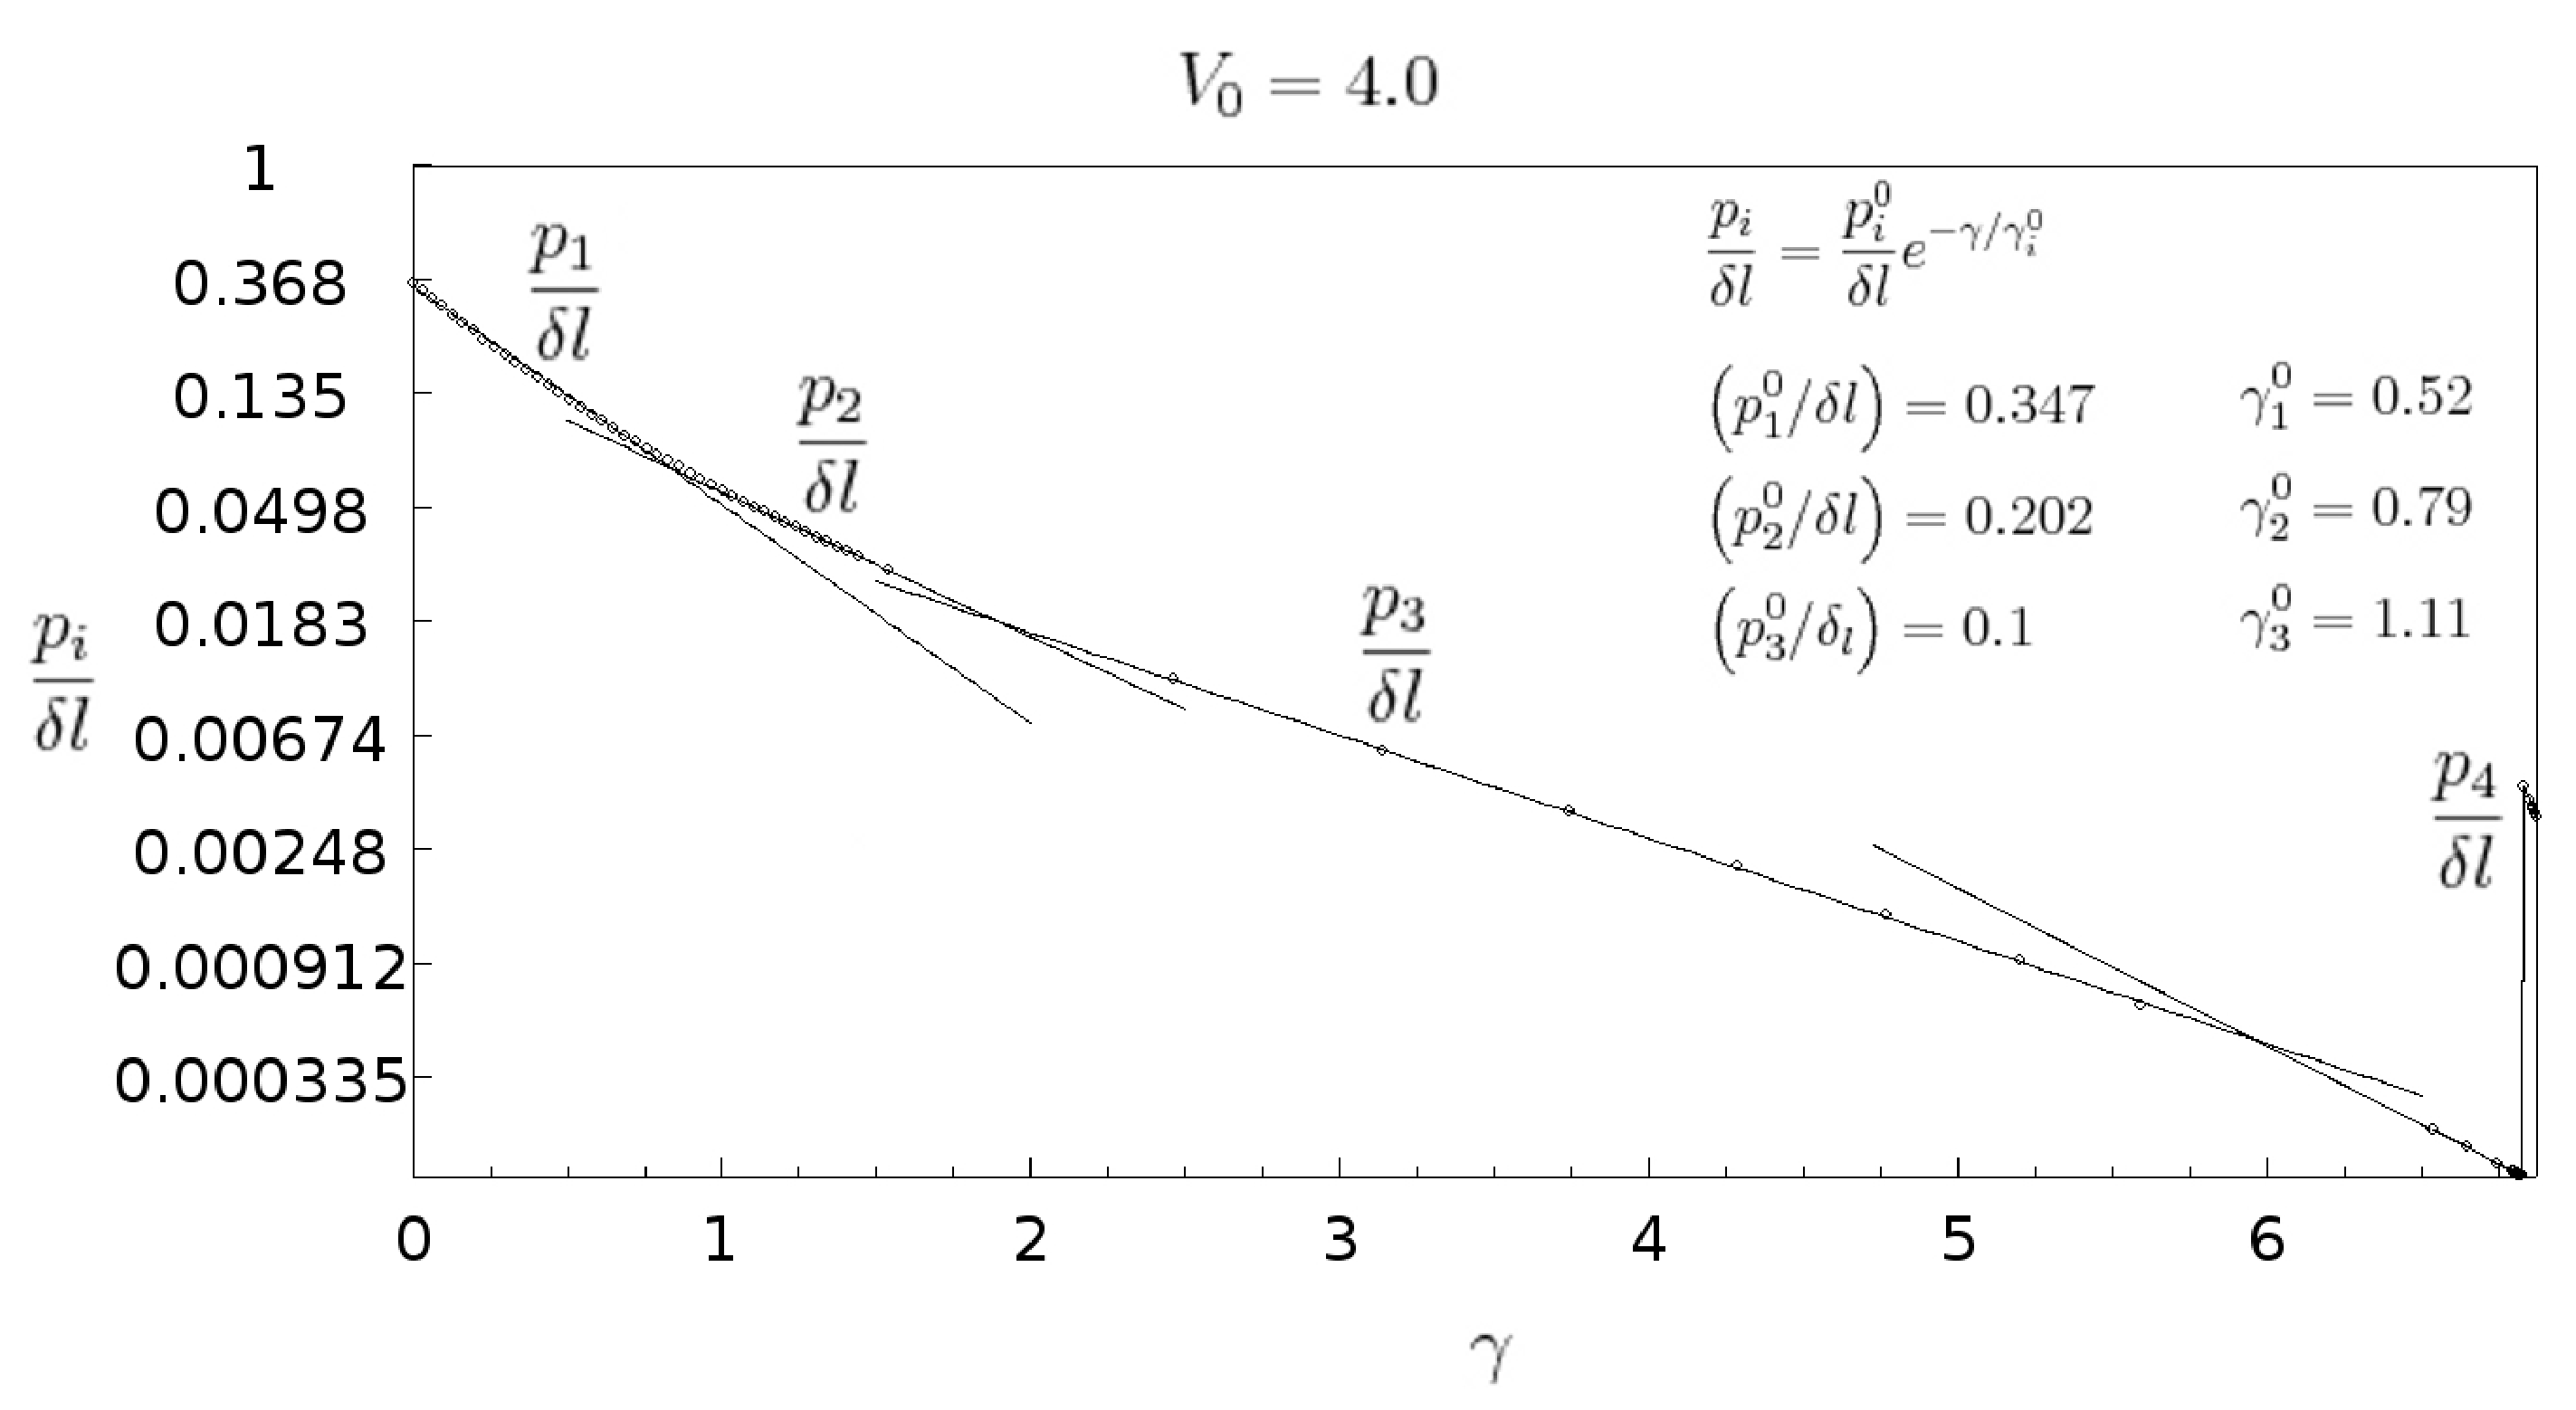
\psfig{file=jpegs/chapter-tof/fig2.eps,height=3.8in,width=5.7in}
\caption{Semi-logarithmic plot of the one dimensional probability density $p_i/{\delta l}$ of two particles being within a rectangular strip of arbitrarily small width $\delta l$ along the line $x_1=x_2$. $p_i/{\delta l}$ is plotted as a function of the strongly interacting parameter $\gamma$ for a constant $V_0=4.0$. The decay rate of the probability $p_i$ changes sharply at 4 regions, labeled by the index $i$. The data points (indicated by circles) have been fitted to exponential decay rates at each region (indicated by lines).The legend provides the numerically fitted values of the decay rates $\gamma^0_i$. Note the discontinuous spike at $\gamma\sim 7$.}
\label{fig:tonksparam:appendixtof}
\end{figure}
Here, $i$ is an index distinguishing different regimes of interest in the $\gamma$-space. Also, $p_i$ is the total probability that the two particles will be together within a rectangular strip along the line $x_1=x_2$ and arbitrarily small width $\delta l$. As expected, it vanishes for large values of $\gamma$.

In this strongly interacting regime, the two particles have no probability of occupying the same position simultaneously. Thus, they act in a way that is similar to a Tonks gas~\cite{tonks:gas}.  The transition to this regime is not consistent, however. We note four distinct ranges of $\gamma$ for which the decay rates of 
$p_i/{\delta l}$  are different. In the first three ranges, $p_i$ seems to be decaying exponentially ie $\left( p_i/{\delta l}\right)=\left( p^0_i/{\delta l} \right) e^{-(\gamma/\gamma^0_i)}$ for $i=1,2,3$. The data points have been fitted to exponents by the use of numerical nonlinear least-squares algorithms.
The decay rate, characterized by $ \gamma^0_i $, decreases sharply at $\gamma\sim 1, 2$ and $6$. Near $\gamma\sim 7$, there is a sharp increase in $p_i$ after which it continues to decrease. If we neglect the probability if it falls below $1/e$ of the maximum, then the 'strongly interacting regime' is achieved beyond $\gamma\sim 0.4$. In our case, we have chosen a $\gamma$ of $5.20142$ for our strongly interacting regime, placing the system in region $3$ of Fig~\ref{fig:tonksparam:appendixtof}. The value of $\left(V_0,U_0\right)$ chosen is $\left(4.0, 40.0\right)$.

The second regime, henceforth referred to as the 'single particle regime', will consist of a weakly attractive system and the well-depth as seen in~\cite{mypaper}. Thus, the parameter values chosen are $\left(7.2912229, -1.0\right)$.The probability distributions of the ground state  $|E_1\rangle$, as well as the excited states  $|E_2\rangle$ and  $|E_4\rangle$, given by Eqn~\ref{eq:hamscale:appendixtof}  are shown in Figs~\ref{fig:wavefunctions_tonks:appendixtof}.a through \ref{fig:wavefunctions_tonks:appendixtof}.c for the strongly interacting regime. Note that, as expected, there is virtually no probability that $x_1=x_2$.
%Fig. 3
\begin{figure}
\ \psfig{file=jpegs/chapter-tof/fig3.eps,height=6.0in,width=3.0in}
\caption{Plots of energy eigenfunctions for the two interacting bosons in a double well potential in the strongly interacting regime. Figures (a) through (c) are contour plots of the probability density $|\langle x_1,x_2|E_1\rangle|^2$ ,  $|\langle x_1,x_2|E_2\rangle|^2$  and $|\langle x_1,x_2|E_4\rangle|^2$ respectively. The probabilities are plotted as functions of $x_1$ and $x_2$. All units for all figures are dimensionless}
\label{fig:wavefunctions_tonks:appendixtof}
\end{figure}
The probability distributions of the first seven quantum energy states of the system in the single particle regime are shown in Figs.~\ref{fig:wavefunctions:appendixtof}.a through  \ref{fig:wavefunctions:appendixtof}.g. Note the plots of the ground state, $|E_1\rangle$, third excited state, $|E_4\rangle$,  and sixth excited state $|E_7\rangle$. The dynamics of the system, when driven by sequential pulses whose energies are tuned to transitions between these states, show the effects of dynamical chaos through level-repulsion in the Floquet eigenphases~\cite{mypaper}. A crossing through the level-repelling region can be avoided if the radiation pulses are applied adiabatically, producing a chaos assisted passage as detailed in~\cite{mypaper}.
%Fig. 4
\begin{figure}
\ \psfig{file=jpegs/chapter-tof/fig4.eps,height=6.0in,width=4.0in}
\caption{Plots of energy eigenfunctions for the two interacting bosons in a double well potential in the single particle regime. All units are dimensionless. Figures (a) through (f) are contour plots of the probability density $|\langle x_1,x_2|E_1\rangle|^2$ through $|\langle x_1,x_2|E_6\rangle|^2$ respectively. Figure (g) is a contour plot of the probability density
$|\langle x_1,x_2|E_7\rangle|^2$.The peaks in the probability are numbered. The probabilities are plotted as functions of $x_1$ and $x_2$. All units for all figures are dimensionless}
\label{fig:wavefunctions:appendixtof}
\end{figure}
%
\section{\label{sec:2:appendixtof} Time of Flight Images} 
%
%
The normalized first order correlation function of a single double well is a measurement of the atomic density $n(x)$. Such correlations can be measured following a STIRAP transition by the time-of-flight (TOF) technique in which the trapped atoms are released sufficiently quickly  that the diabatic approximation in quantum mechanics can be applied. The atoms then expand ballistically until they reach a detection plate. If the plate is far enough from the double well system that the far-field approximation can be used, then the Green's Function for the system can be simplified and the time translation reduced to a simple Fourier Transform.  If the 'detector plane' coordinates are denoted by unprimed variables $\left[ x_1,x_2,t \right]$ and the double -well coordinates by primed variables $\left[ x'_1,x'_2,t \right]$ for a 2-particle system after all the external fields and traps have been diabatically switched off, and the interactions between the atoms rendered negligible by tuning a homogenous magnetic field close to the Feshbac resonance that adds an attractive amplitude to the normally repulsive point contact pseudopotential~\cite{feshbach:resonance}~\cite{pethick:bec}. The system then evolves ballistically in free space. 

The Green's Function or Propagator $G({\bf x},t;{\bf x}',t')$ is defined by
\begin{equation}
\Psi ({\bf x},t) = \int d^2x \mbox{ } G({\bf x},t;{\bf x}',t') \Psi ({\bf x}',t'),
\label{eq:greensfunction:appendix}
\end{equation}
where ${\bf x} = \left[ x_1, x_2 \right]$, and $\Psi({\bf x},t)$ is the wavefunction, with similar expressions for the primed coordinates. For free space, the relevant 1-dimensional Schr\"odinger equation for 2-particles is
\begin{eqnarray}
\left[ H-i\frac{\partial}{\partial t} \right] \Psi({\bf x},t) =0, \nonumber \\
H=-\left[ \frac{\partial^2}{\partial x^2_1} + \frac{\partial^2}{\partial x^2_2} \right].
\end{eqnarray}
 Thus, the Green's function~\cite{sakurai} will be the solution to
 \begin{equation}
 \left[ H-i\frac{\partial}{\partial t} \right] G({\bf x},t;{\bf x}',t') = \delta ({\bf x}-{\bf x}') \delta (t-t').
 \label{eq:greens:appendix}
 \end{equation}
The solution to Eqn~\ref{eq:greens:appendix} in free space is
\begin{equation}
G({\bf x},t;{\bf x}',t') = \frac{\sqrt{-i}}{L} \exp{\left[ i\pi | \frac{{\bf x}-{\bf x}'}{L}|^2 \right]}.
\label{eq:greensfn:appendix}
\end{equation}
Here, the ballistic de-Broglie equation,
\begin{equation}
L^2=4 \pi \tau,
\label{eq:debroglie:appendixtof}
\end{equation}
 provides the relation between the detector-system separation $L$ and the time-of-flight $\tau=\left(t-t'\right)$.

Now, consider such a two particle system localized at a site $j$. The wavefunction is localized about ${\bf x}'_j = \left[ x'_j, x'_j \right]$ and can be written in the form $\Psi({\bf x}'-{\bf x}'_j)$. We now use Eqns~\ref{eq:greensfn:appendix} and~\ref{eq:debroglie:appendixtof} on Eqn~\ref{eq:greensfunction:appendix}, and apply the shift theorem for Fourier transforms~\cite{goodman}~\cite{Grondalski:etal} to get
\begin{equation}
\Psi(x,\tau) = \sqrt{\frac{-i}{4\pi\tau}}\exp{\left[ i\frac{1}{2\tau}\left( \frac{|{\bf x}|^2}{2} + {\bf x}\bullet {\bf x}'_j\right)\right]} F\left[ \Psi({\bf x}')\right]_{{\bf u}=\frac{{\bf x}}{4\pi\tau}},
\label{eq:TOF:appendixtof}
\end{equation}
where the primed coordinates refer to the double well system, the unprimed coordinates refer to the detector, and $ F\left[ \Psi({\bf x}')\right]_{\bf u}$ is the Fourier transform
\begin{equation}
F\left[ \Psi({\bf x}')\right]_{\bf u} \equiv \frac{1}{2 \pi} \int d^2x' \Psi({\bf x}') e^{i{\bf u}\bullet{\bf x}'}.
\label{eq:ft:appendix}
\end{equation}
In the equation above,  ${\bf u} = \left[ u_1, u_2 \right]$ is the momentum space vector. For a large collection of such systems, each in the desired pure state, the measured TOF is simply the probability obtained from Eqn~\ref{eq:TOF:appendixtof} times the number of such double wells $N$ (which we shall subsequently drop off as an appropriately adjusted overall normalization).
\begin{equation}
n({\bf x})= N \frac{1}{4\pi\tau} | F\left[ \Psi({\bf x}') \right]_{{\bf u}=\frac{{\bf x}}{4\pi\tau}} |^2.
\label{eq:TOFmeas:appendixtof}
\end{equation}

We note that there are noticeable differences in the symmetries of the two states $|E_4\rangle$ and $|E_7\rangle$ (refer to Figs~\ref{fig:wavefunctions:appendixtof}). The distinctly resolved peaks in each wavefunction (labeled $1$ through $8$ for $|E_7\rangle$) can be approximated by elliptical Gaussian functions. Thus, the wavefunction can be represented by  a two-dimensional function as follows:
\begin{equation}
\Psi(x'_1, x'_2) = \sum_{i=1}^{R} {a_i}G\left( x'_1, x^i_1, \alpha^i_1\right) G\left( x'_2, x^i_2, \alpha^i_2\right),
\label{eq:gaussianfits:appendixtof}
\end{equation}
where
\begin{equation}
G(x,x^i,\alpha) =\left( \frac{2\alpha}{\pi}\right)^{1/4} e^{-\alpha \left(x-x^i \right)^2}.
\end{equation}
Here, $R$ is the number of peaks (8 for $|E_7\rangle$). Also,  we have rotated our coordinate system to the axes of symmetry (by $45$ degrees) of $|E_7\rangle$. Using the well-known relation for the Fourier transform of a Gaussian applied to Eqns~\ref{eq:TOFmeas:appendixtof} and~\ref{eq:gaussianfits:appendixtof}, we get (sans any overall normalizations), 
\begin{equation}
n(x_1,x_2) = | \sum_{j=1}^{R} a_j \left(\frac{1}{4\pi^2 \alpha^j_1\alpha^j_2}  \right)^{1/4} e^{i\frac{x_1x^j_1 + x_2x^j_2}{4\pi\tau}} e^{-\frac{x^2_1}{16\pi^2 \alpha^j_1\tau^2}} e^{-\frac{x^2_2}{16\pi^2 \alpha^j_2\tau^2}} |^2.
\label{eq:gaussianfitsexpand:appendixtof}
\end{equation}
We rewrite this as 
\begin{eqnarray}
n(x_1,x_2)=| \sum_{j=1}^R r_j(x_1,x_2) e^{i k_j x_1} |^2, \nonumber \\
r_j(x_1,x_2)=a_j \left( \frac{1}{4\pi^2\alpha^j_1\alpha^j_2} \right)^{1/4} e^{i\frac{x_2 x^j_2}{4\pi\tau}} e^{-\frac{x^2_1}{16\pi^2\alpha^j_1\tau^2}} e^{-\frac{x^2_2}{16\pi^2\alpha^j_2\tau^2}}, \nonumber \\
k_j = \frac{ x^j_1}{4\pi\tau}.
\label{eq:rthetasplit:appendixtof}
\end{eqnarray}
The expression above can be simplified to 
\begin{equation}
n(x_1,x_2)=\sum_{j=1}^{R}|r_j(x_1,x_2)|^2 + \sum_{\left\langle i,j \right\rangle} 2r^*_i(x_1,x_2) r_j(x_1,x_2) |\cos{(k_j-k_i)x}|.
\end{equation}
In order to get the density functional $n(x)$, we integrate out the $x_2$ (symmetries guarantee that the result will be the same if we integrate $x_1$ instead) and get
\begin{eqnarray}
n(x)=\sum_{j=1}^{R}r^2_j(x) + \sum_{\left\langle i,j \right\rangle} 2r^2_{ij}(x) |\cos{(k_j-k_i)x}|,
\label{eq:interesting:appendixtof}
\end{eqnarray}
where $\left\langle i,j \right\rangle$ are distinct (ie $i \neq j$) combination pairs of peaks. In the equation above, integrating $x_2$ by Gaussian integral methods leaves out a Gaussian dependencies in $x$ of $r_j$ and $r_{ij}$ (the subscripts for $x$ have been dropped). Thus,
\begin{eqnarray}
r^2_j(x) = \tau a^2_j \sqrt{\frac{4\pi}{\alpha^j_1}}  e^{-\frac{x^2}{16\pi^2\alpha^j_1\tau^2}}, \nonumber \\
r^2_{ij}(x)=2 \tau a_i a_j \left(\frac{1}{ \alpha^i_1 \alpha^j_1 \alpha^i_2 \alpha^j_2} \right)^\frac{1}{4} \sqrt{\pi\alpha^{ij}_2} e^{-\frac{\alpha^{ij}_2(x^j_2-x^i_2)^2}{4}} e^{-\frac{x^2}{16 \pi^2 \alpha^{ij}_1\tau^2}},
\end{eqnarray}
where we have defined
\begin{equation}
\frac{1}{\alpha^{ij}}\equiv \frac{1}{\alpha^i}+\frac{1}{\alpha^j}.
\end{equation}

From the plot of $|E_7\rangle$ for the single particle regime (see Fig~\ref{fig:wavefunctions:appendixtof}), we notice that there are only three distinct kinds of peaks (labeled $1$, $5$ and $8$). Thus there are three pairs whose $k$'s are unequal viz. $\left\langle 1,5 \right\rangle$ and $\left\langle 1,8 \right\rangle$ and $\left\langle 5,8 \right\rangle$. All other terms are absorbed into the perfect square terms in Eqn~\ref{eq:interesting:appendixtof}. Each such term is a Gaussian centered at $x=0$ with varying widths. If we look at values of $x$ sufficiently far from the center of the detector plate, those terms drop off quickly, leaving just the three oscillatory terms. This signal will be distinct from that obtained from the TOF of state $|E_4\rangle$, which has only $2$ such term (only $2$ distinct kinds of peaks). If the time-of-flight $\tau$ is chosen so that the values of $k_j-k_i$ are small, then the signal will look like an amplitude modulated sinusoid. 

\section{\label{sec:3:appendixtof} Time-of-Flight: Numerical Plots}
This section will detail the procedure for obtaining numerical plots of the tof distributions of the eigenstates of the double well system. The two boson problem in a double well is diagonalized as detailed in section~\ref{chapter-dblwell:diaghamilt} of chapter~\ref{chapter-dblwell}, and appendix~\ref{appendix-matelements}. Thus, the eigenfunctions are obtained as linear superpositions of the eigenfunctions of two bosons in a box of appropriately chosen length $L$, ie
\begin{eqnarray}
{\langle}x_1,x_2\vert n_1,n_2{\rangle} ^{(s)}=\frac{1}{\sqrt{2(1+\delta_{n_1,n_2})}} 
[{\langle}x_1|n_1\rangle{\langle}x_2|n_2\rangle +{\langle}x_1|n_2\rangle{\langle}x_2|n_1\rangle ], \nonumber \\
\langle x|n\rangle=\frac{1}{\sqrt{L}} \sin{\biggl[}{\frac{n\pi}{2}(\frac{x}{L}-1){\biggr]}},
\label{eq:pboxfn:appendix}
\end{eqnarray}
 if $|x_i|<L$, and $0$ otherwise. Thus, the final solution to an eigenfunction $|E_n\rangle$ of the double well will be a linear superposition of the  'finite wave train'  functions defined above, ie
\begin{equation}
\langle x_1,x_2|E_n\rangle =  \sum_{\left[n_1,n_2\right]=\left[1,1\right]}^{\left[ N,N \right]} C^{\left[n_1,n_2 \right]}_{E_j} {\langle}x_1,x_2\vert n_1,n_2{\rangle} ^{(s)},
\end{equation}
where the $C^{\left[n_1,n_2 \right]}_{E_j}$ are obtained numerically using the nonadaptive finite element method. This result can then be substituted into Eqn~\ref{eq:TOFmeas:appendixtof} to get
\begin{equation}
n(x_1,x_2) = N \frac{1}{4\pi\tau} |\sum_{\left[n_1,n_2\right]=\left[1,1\right]}^{\left[ N,N \right]} C^{\left[n_1,n_2 \right]}_{E_j} F\left[ {\langle}x'_1,x'_2\vert n_1,n_2{\rangle} ^{(s)} \right]_{\left[u_1,u_2\right]=\frac{\left[ x_1,x_2 \right]}{4\pi\tau}}|^2.
\label{eq:density:appendix}
\end{equation}
Using the linearity of Fourier Transforms and Eqn~\ref{eq:pboxfn:appendix}, we get
\begin{multline}
F\left[ {\langle}x'_1,x'_2\vert n_1,n_2{\rangle} ^{(s)} \right]_{\bf u}=\frac{1}{\sqrt{2(1+\delta_{n_1,n_2})}}\\
\left( F[{\langle}x_1|n_1\rangle]_{u_1} F[{\langle}x_2|n_2\rangle]_{u_2} +F[{\langle}x_1|n_2\rangle]_{u_1} F[{\langle}x_2|n_1\rangle]_{u_2}  \right).
\label{eq:ft:appendix}
\end{multline}
The Fourier transform of the finite wave train ($\langle x|n\rangle$ in Eqn~\ref{eq:pboxfn:appendix}) can be calculated using Gaussian integrations~\cite{arfken} to yield
\begin{equation}
F[\langle x' | n \rangle]_u = \frac{1}{\sqrt{2L\pi}}  \frac{1}{\left( \frac{n^2 \pi^2}{4 L^2}-u^2 \right) } \left[ 2u \sin{\frac{n \pi}{2}}-\frac{n \pi}{L} \sin{L u} \right],
\label{eq:pboxft:appendixtof}
\end{equation}
where $u$ is the momentum space vector. Thus, by plugging Eqn~\ref{eq:pboxft:appendixtof} into Eqn~\ref{eq:ft:appendix}, and that into Eqn~\ref{eq:density:appendix}, the tof distribution $n(x_1,x_2)$ can be obtained, the final density distribution is the density functional average of this result viz.
\begin{equation}
n(x)=\int dx' n(x, x').
\end{equation}
Thus, a numerical expression for Eqn~\ref{eq:TOFmeas:appendixtof} was obtained for two degrees of freedom $x_1$ and $x_2$, and the density functional $n(x)$ determined by integrating out one of the coordinates by adaptive Gauss-Kronrod quadrature. 

Numerical results for the tof distributions of the eigenstates of the double well for the strongly interacting and single particle regimes are shown in Figs~\ref{fig:tof_1lakh_tonks:appendixtof} and ~\ref{fig:tof_1lakh:appendixtof} respectively. The distributions are shown for tof $\tau=10^5$ units of $T_u$. All the dynamics is essentially independent of the characteristic length scale $L_u$ (the actual position of the well minima). For practical reasons, we choose an $L_u$ of $50$ $nm$~\cite{mypaper}. Consequently, with a Rubidium-85 atomic mass of $85.4678$ $g·mol^{-1}$, we get a $T_u$ of about $6.7$  $\mu s$, which makes $\tau$ to be $0.67$ seconds. Using Eqn~\ref{eq:debroglie:appendixtof}, we get a detector distance of about $2.2$ $cm$. 

Figures~\ref{fig:tof_1lakh_tonks:appendixtof}(a) through (c) show the tof distributions of the states $| E_1\rangle$, $| E_2\rangle$, and $| E_4\rangle$ respectively for the strongly interacting gas detailed in section 1. Note that the the momentum distribution of $| E_1\rangle$, closely approximates the Heavyside function that is characteristic of the momentum distribution of a Tonks gas~\cite{tonks:gas} (barring the lack of any occupancy at zero momentum, which is forbidden in this case due to a nonzero value of the ground state energy $E_1$).

Figures~\ref{fig:tof_1lakh:appendixtof}(a) through (c) show the tof distributions of the states $| E_1\rangle$, $| E_4\rangle$, and $| E_7\rangle$ respectively in the single particle regime detailed in section 1.Note that, as predicted by the calculations in section~\ref{sec:2}, the number of distinct oscillations in each distribution correspond to the number of distinct pairs of peaks seen in the wavefunctions. Thus, each state generates a particular signature in the tof. Since the transitions to $|E_4\rangle$   and $|E_7\rangle$ are caused by crossing or avoiding a chaos assisted adiabatic passage, the amplitude modulation in the tof differentiates between the two outcomes. In case there is an incoherent excitation, there will be large numbers of overlapping or closely spaced peaks and the oscillations will constructively interfere everywhere, thus distinguishing the resultant signal from one obtained by the TOF of a coherent excitation. Thus,  the influence (or lack thereof) of chaos in the underlying classical dynamics can be indirectly inferred by the one extra oscillation in Fig~\ref{fig:tof_1lakh:appendixtof}(c) compared to Fig~\ref{fig:tof_1lakh:appendixtof}(b).

Time of flight fluorescence methods for profiling the wavefunction, such as measuring the momentum distribution by interrupting the particle flow with counter-propagating laser beams and then measuring fluorescence as a function of time (time of flight absorption)~\cite{fluorescense}~\cite{fluorescense:web}, will have high signal to noise ratio (compared to absorption)~\cite{raizen}.  Single shot fluorescence images should duplicate the profile shown in Figs~\ref{fig:tof_1lakh:appendixtof}(a)-(c) for a double well system produced by optical lattices. For a single magnetically confined double well, repeated measurements of position by the means of atom detectors, or by performing scanning tunneling microscopy on an appropriate substrate where the atoms are allowed to deposit after their tof expansion, should reproduce the required results.
\pagebreak
%Fig 1 (repeat from previous chapter)
%\begin{figure} 
%\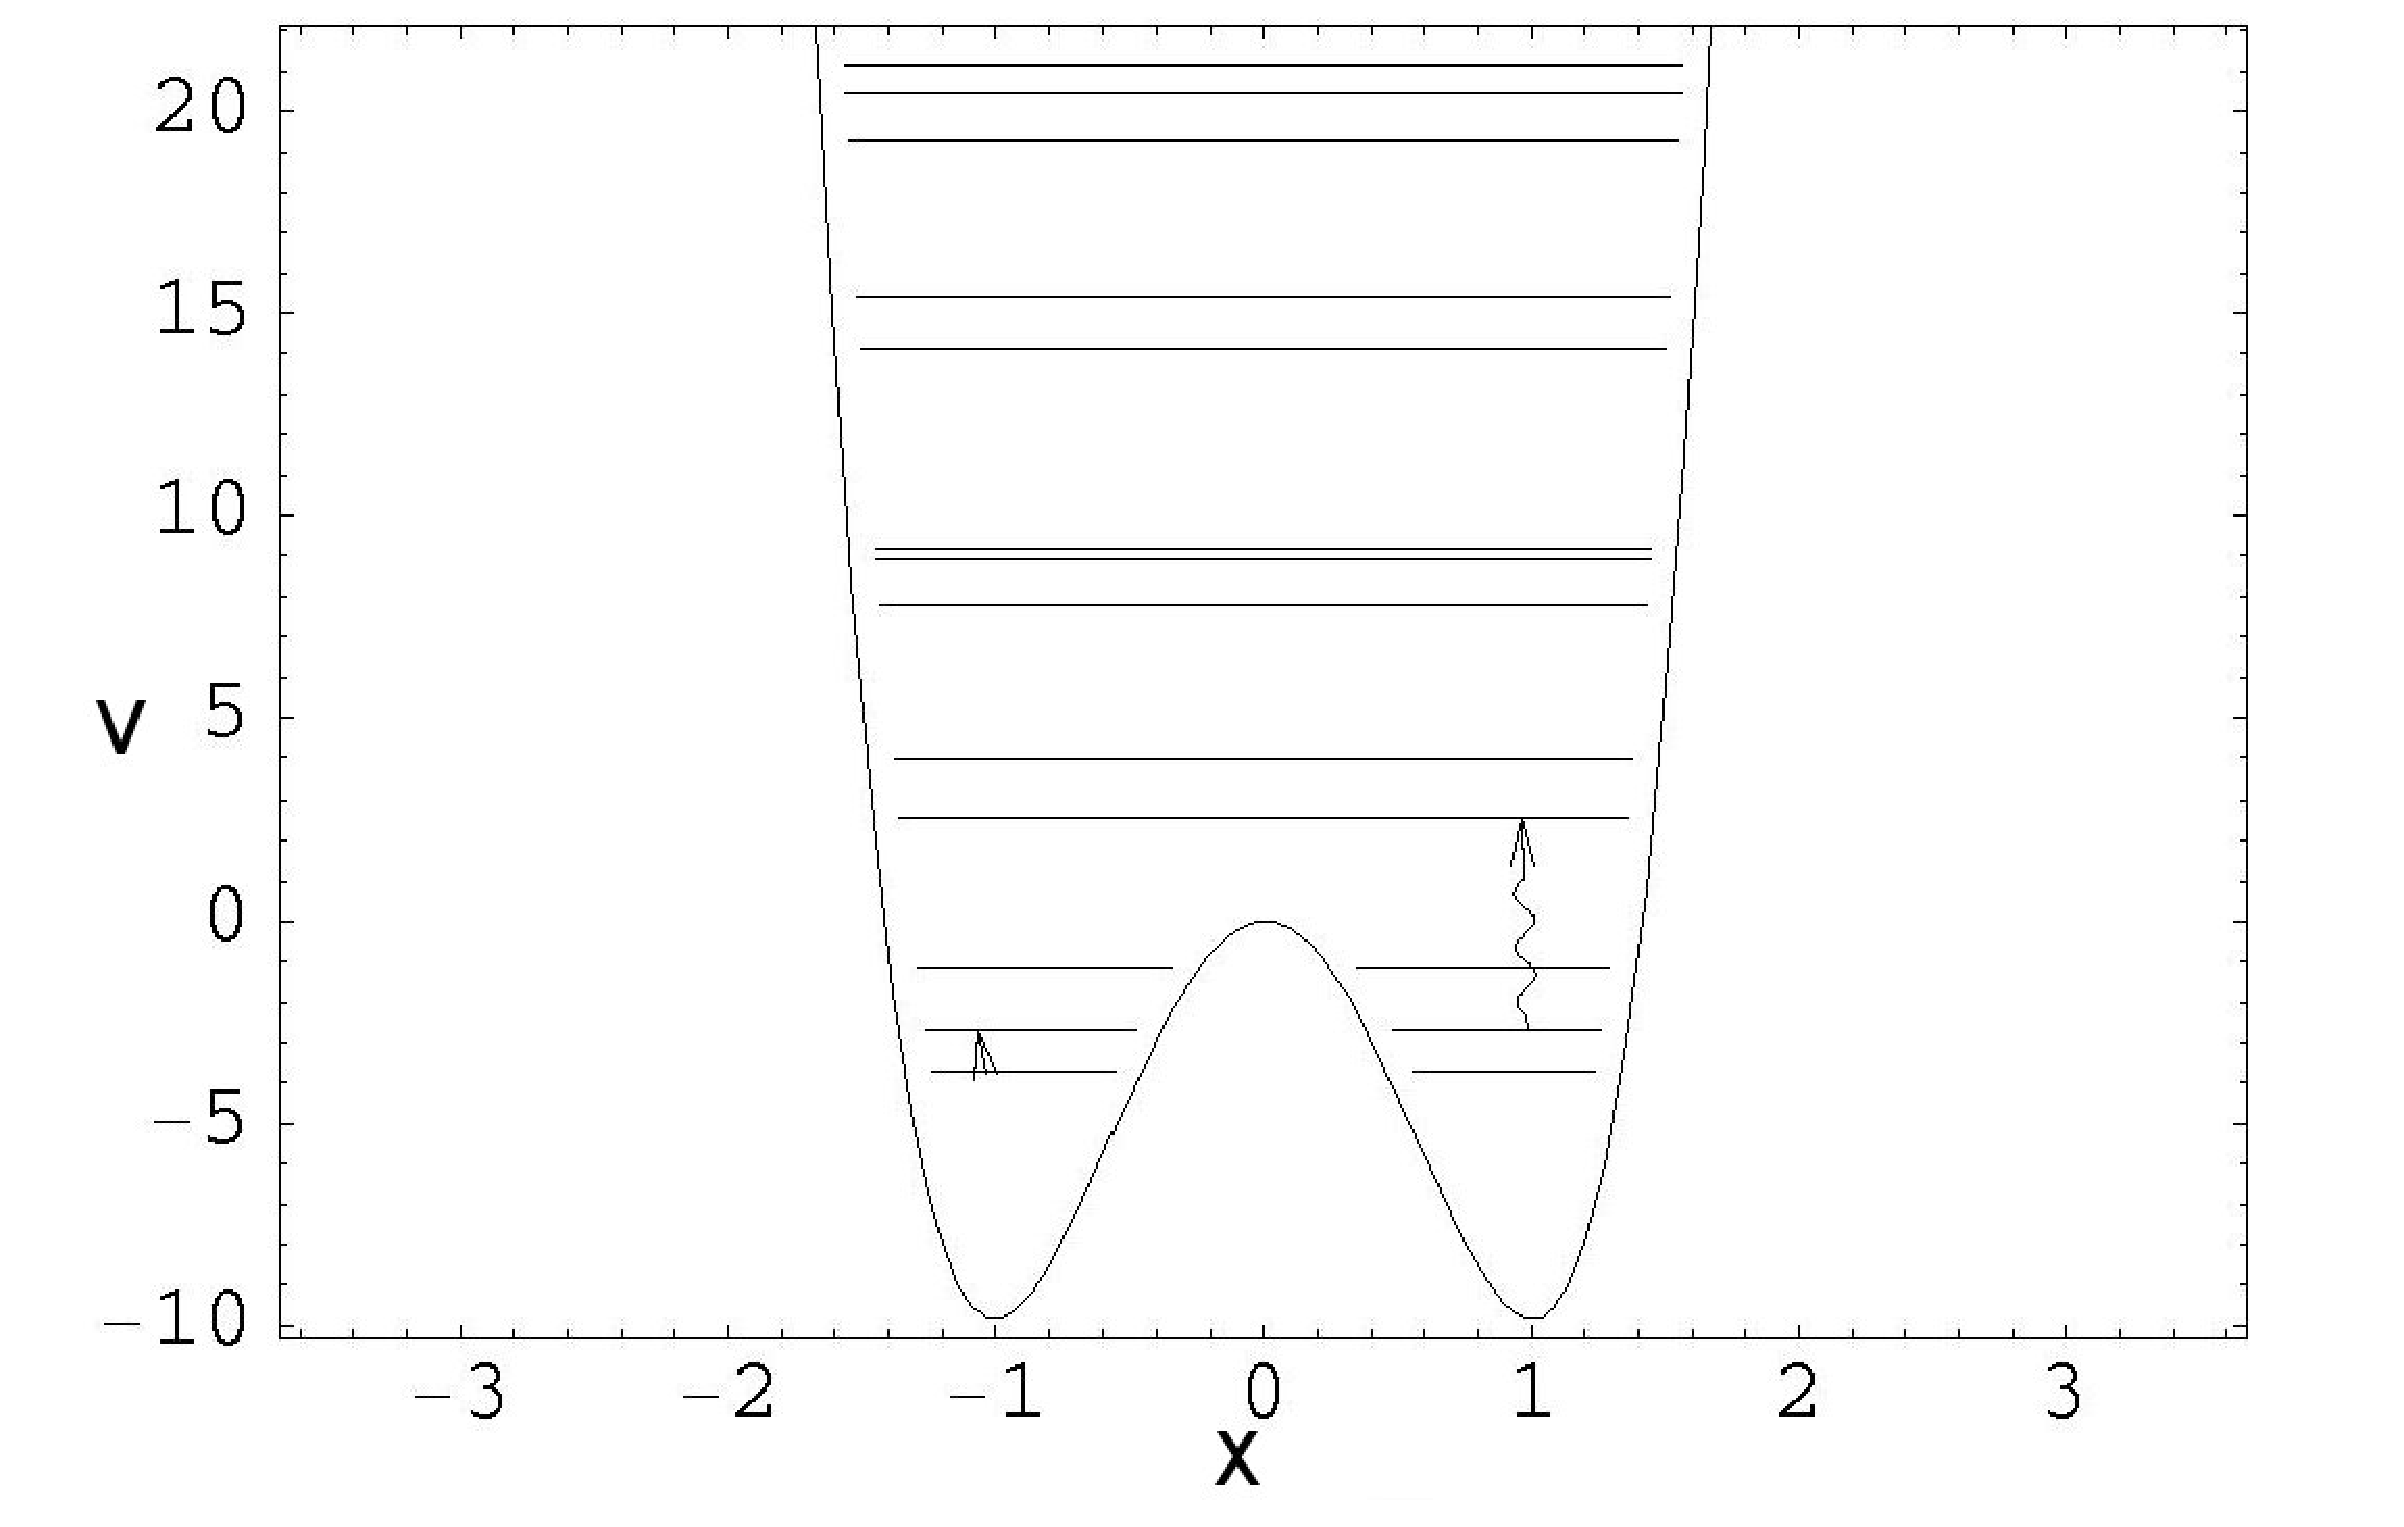
\psfig{file=jpegs/chapter-tof/fig1.eps,height=3.0in,width=5.0in}
%\caption{Plot of the double-well potential experienced by each boson in case 2. The energy levels, $E_1=-6.42262$, $E_2=-5.68883$ and $E_4=0.640055$  of the interacting two-boson system (interaction strength  $U_0=-1.0$) are also sketched, with wavy arrows denoting the levels connected by the STIRAP pulses. Note the slightly detuned resonance between the $2 \leftrightarrow 4$ and the $4 \leftrightarrow 7$ levels where $E_7=6.96998$. Here, $V_0=7.2912229$.}
%\label{fig:doublewell_case02}
%\end{figure}

%Fig. 5
\begin{figure}
\ \psfig{file=jpegs/chapter-tof/fig5.eps,height=6.0in,width=4.0in}
\caption{Figures (a) through (c) are plots of the one-dimensional time-of-flight distributions for the double-well eigenstates $| E_1\rangle$, $| E_4\rangle$ and $| E_7\rangle$ respectively in the strongly interacting regime. The distributions are symmetric about $x=0$, so only the positive half is shown. The number density $n(x)$ in the ordinate is for $10^6$ double wells after a time of flight $\tau = 10^5$ (in units of $T_u$). The abscissa is shown in dimensionless units of $L_u$. }
\label{fig:tof_1lakh_tonks:appendixtof}
\end{figure}

%Fig. 6
\begin{figure}
\ 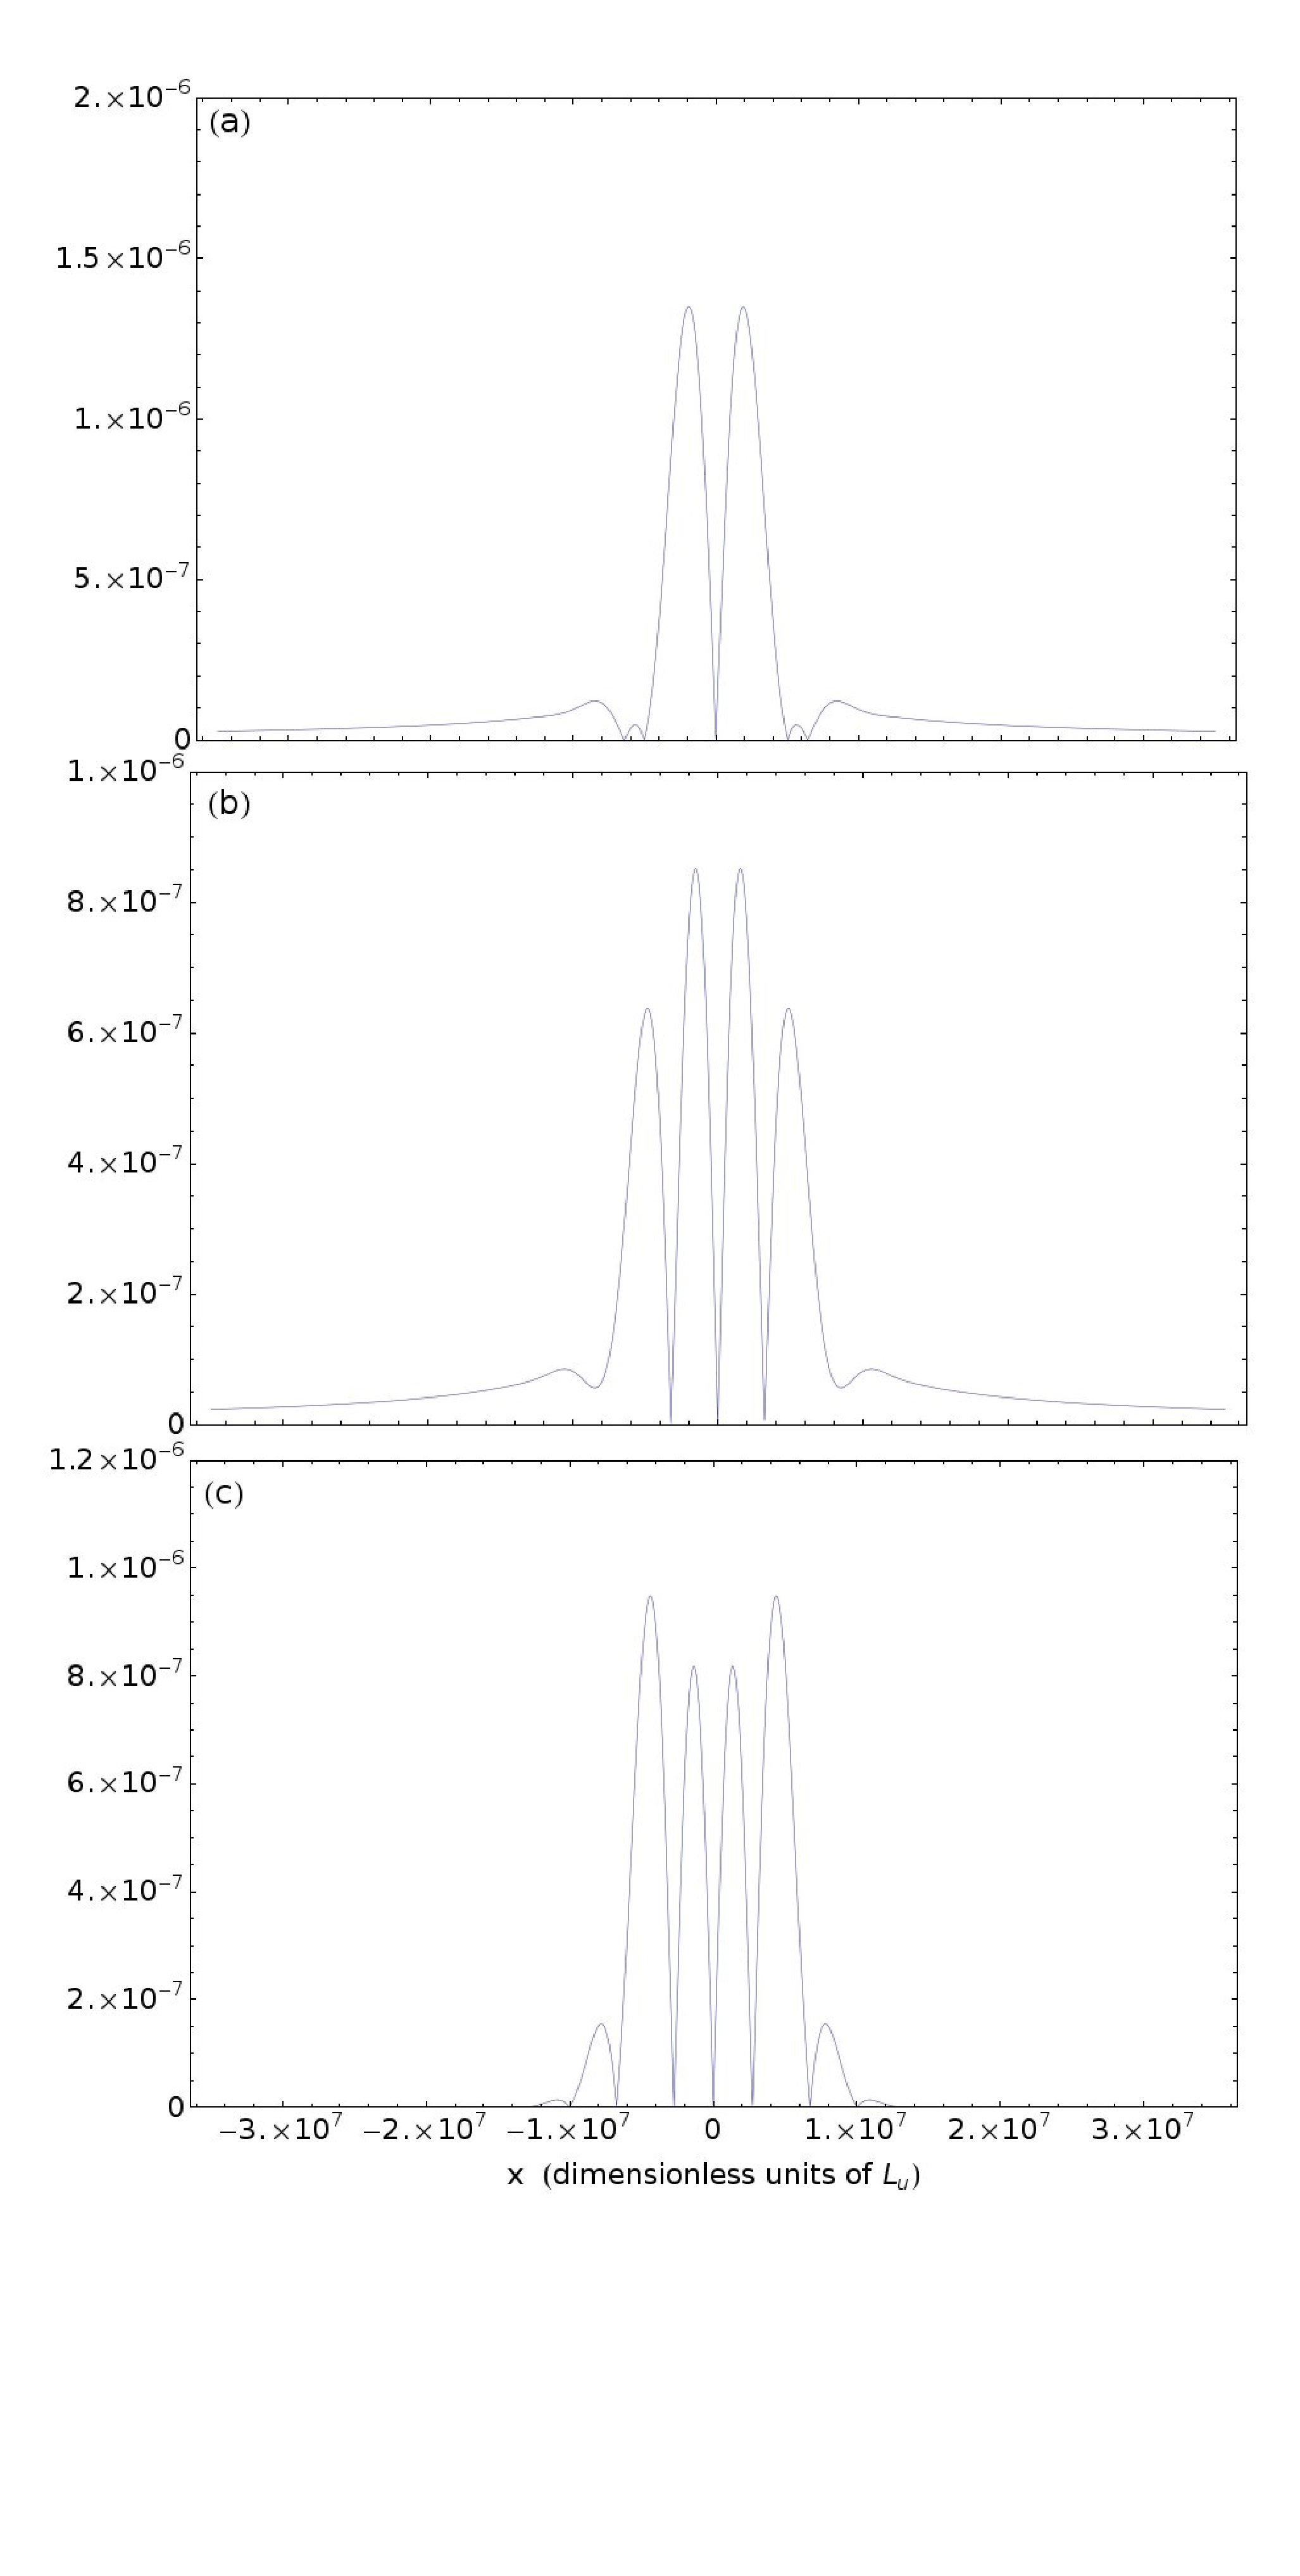
\psfig{file=jpegs/chapter-tof/fig6.eps,height=6.0in,width=4.0in}
\caption{Figures (a) through (c) are plots of the time-of-flight distributions for the double-well eigenstates $| E_1\rangle$, $| E_4\rangle$ and $| E_7\rangle$ respectively in the single particle regime. The number density $n(x)$ in the ordinate is for $10^6$ double wells after a time of flight $\tau = 10^5$ (in units of $T_u$). The abscissa is shown in dimensionless units of $L_u$.}
\label{fig:tof_1lakh:appendixtof}
\end{figure}



%%%%%%%%%%%%%%%%%%%%%%%%%%%%%%%%%%%%%%%%%%%%%%%%%%%%%%%%%%%%%%%%%%%%%%
% Generate the bibliography.					     %
%%%%%%%%%%%%%%%%%%%%%%%%%%%%%%%%%%%%%%%%%%%%%%%%%%%%%%%%%%%%%%%%%%%%%%
%								     %
% NOTE: For master's theses and reports, NOTHING is permitted to     %
%	come between the bibliography and the vita. The command      %
%	to generate the index (if used) MUST be moved to before      %
%	this section.						     %
%								     %
\nocite{*}      % This command causes all items in the 		     %
                % bibliographic database to be added to 	     %
                % the bibliography, even if they are not 	     %
                % explicitly cited in the text. 		     %
		%						     %
\bibliographystyle{unsrt}  % Here the bibliography 		     %
\bibliography{diss}        % is inserted.			     %
\index{Bibliography@\emph{Bibliography}}%			     %
%%%%%%%%%%%%%%%%%%%%%%%%%%%%%%%%%%%%%%%%%%%%%%%%%%%%%%%%%%%%%%%%%%%%%%

%%%%%%%%%%%%%%%%%%%%%%%%%%%%%%%%%%%%%%%%%%%%%%%%%%%%%%%%%%%%%%%%%%%%%%
% Generate the index.						     %
%%%%%%%%%%%%%%%%%%%%%%%%%%%%%%%%%%%%%%%%%%%%%%%%%%%%%%%%%%%%%%%%%%%%%%
%								     %
% NOTE: For master's theses and reports, NOTHING is permitted to     %
%	come between the bibliography and the vita. This section     %
%	to generate the index (if used) MUST be moved to before      %
%	the bibliography section.				     %
%								     %
\printindex%    % Include the index here. Comment out this line      %
%		% with a percent sign if you do not want an index.   %
%%%%%%%%%%%%%%%%%%%%%%%%%%%%%%%%%%%%%%%%%%%%%%%%%%%%%%%%%%%%%%%%%%%%%%


%%%%%%%%%%%%%%%%%%%%%%%%%%%%%%%%%%%%%%%%%%%%%%%%%%%%%%%%%%%%%%%%%%%%%%
% Vita page.							     %
%%%%%%%%%%%%%%%%%%%%%%%%%%%%%%%%%%%%%%%%%%%%%%%%%%%%%%%%%%%%%%%%%%%%%%

\begin{vita}
Analabha Roy
was born in Mumbai (formerly Bombay), Maharashtra, India on 21 March 1978, the son of
Professor Probir Roy and Professor Manashi Roy.  He received the Bachelor
of Science degree in Physics from Jadavpur University, Kolkata (formerly Calcutta), India and 
the Master of Science degree in Physics from the Indian Institute of Technology, Kanpur, India,
He applied to the University of Texas at Austin for enrollment
in their physics graduate program in 2002. He was accepted and started graduate studies in
September, 2002.

\end{vita}

\end{document}
